\documentclass[11pt,twoside,openany]{book}
\usepackage[T1]{fontenc}
\usepackage[utf8]{inputenc}
\usepackage{tgpagella}
\usepackage[scaled=0.95]{inconsolata}
\usepackage[letterpaper,margin=1.1in]{geometry}
\usepackage{microtype}
\usepackage{amsmath,amssymb,amsthm}
\usepackage{booktabs}
\usepackage{array}
\usepackage{enumitem}
\usepackage[dvipsnames]{xcolor}
\usepackage{tikz}
\usetikzlibrary{positioning,arrows.meta,calc,fit,shapes.multipart,shapes.geometric,decorations.pathreplacing}
\usepackage{listings}
\usepackage[most]{tcolorbox}
\usepackage{caption}
\usepackage{titlesec}
\usepackage{fancyhdr}
\usepackage[hidelinks]{hyperref}
\usepackage{bookmark}
\usepackage[nameinlink]{cleveref}

\setlist{itemsep=2pt,topsep=4pt}
\setlength{\parskip}{0.45em}
\setlength{\parindent}{0pt}
\setlength{\emergencystretch}{2em}

\definecolor{accent}{HTML}{1F4E79}
\definecolor{boxbg}{HTML}{F4F7FB}
\definecolor{ideabg}{HTML}{FFF8E7}
\definecolor{statusbg}{HTML}{EEF6EE}

\titleformat{\chapter}[display]{\normalfont\bfseries\color{accent}}{\large\scshape Chapter \thechapter}{0.4em}{\huge}
\titlespacing*{\chapter}{0pt}{-10pt}{24pt}
\titleformat{\section}{\normalfont\Large\bfseries\color{accent}}{\thesection}{0.8em}{}
\titleformat{\subsection}{\normalfont\large\bfseries}{\thesubsection}{0.8em}{}

\pagestyle{fancy}
\fancyhf{}
\fancyhead[LE,RO]{\thepage}
\fancyhead[RE]{\small\scshape OntoDB: Database Internals by Example}
\fancyhead[LO]{\small\scshape\nouppercase{\leftmark}}
\renewcommand{\headrulewidth}{0.3pt}

% The running example: how OntoDB does it.
\newtcolorbox{ontodb}[1][]{enhanced,breakable,colback=boxbg,colframe=accent,
  boxrule=0.6pt,arc=2pt,left=8pt,right=8pt,top=6pt,bottom=6pt,
  title={In OntoDB#1},fonttitle=\bfseries\small,coltitle=white}
% The one idea to keep from a section.
\newtcolorbox{keyidea}{enhanced,breakable,colback=ideabg,colframe=Goldenrod!70!black,
  boxrule=0.5pt,arc=2pt,left=8pt,right=8pt,top=5pt,bottom=5pt,
  title={Key idea},fonttitle=\bfseries\small,coltitle=black,colbacktitle=Goldenrod!25}
% What is built today and what is planned.
\newtcolorbox{status}{enhanced,breakable,colback=statusbg,colframe=ForestGreen!70!black,
  boxrule=0.5pt,arc=2pt,left=8pt,right=8pt,top=5pt,bottom=5pt,
  title={Status},fonttitle=\bfseries\small,coltitle=white}

\lstset{basicstyle=\ttfamily\small,columns=fullflexible,keepspaces=true,
  frame=single,framerule=0.4pt,rulecolor=\color{black!25},backgroundcolor=\color{black!3},
  xleftmargin=6pt,xrightmargin=6pt,aboveskip=8pt,belowskip=8pt,
  commentstyle=\color{black!55}\itshape,keywordstyle=\color{accent}\bfseries,
  showstringspaces=false,breaklines=true}
\lstdefinelanguage{pseudo}{morekeywords={function,if,else,then,for,each,while,return,do,end,and,or,not,in},
  sensitive=true,morecomment=[l]{//}}

\newcommand{\code}[1]{\texttt{#1}}
\newcommand{\term}[1]{\emph{#1}}

\tikzset{
  page/.style={draw,minimum width=1.25cm,minimum height=0.6cm,font=\scriptsize\ttfamily},
  node box/.style={draw,rectangle split,rectangle split horizontal,rectangle split parts=#1,
    font=\scriptsize\ttfamily,inner sep=3pt,fill=white},
  arrow/.style={-{Stealth[length=2mm]},thick},
}


\title{\color{accent}\Huge\bfseries OntoDB\\[0.4em]
  \LARGE Database Internals by Example\\[1.2em]
  \large\mdseries Storage, indexing, query processing, concurrency, and recovery,\\
  taught through a database management system for ontologies}
\author{Lam Nguyen}
\date{}

\begin{document}
\frontmatter
\maketitle
\tableofcontents
\listofdecisions
\chapter*{Preface}
\addcontentsline{toc}{chapter}{Preface}
\markboth{Preface}{Preface}

A database engine is a small number of ideas, applied with care. Data lives in
fixed-size pages because disks move blocks. A buffer pool keeps the hot pages
in memory because memory is fast and small. A B+ tree turns a key into a page
in three or four reads because its fanout is in the hundreds. A lock manager
makes concurrent transactions look sequential. A write-ahead log, and an
algorithm called ARIES, make a committed transaction survive a crash that
happens at any instant.

This book explains those ideas from the ground up, and it explains each one
twice: first as theory, then as it appears in a real system. The real system
is \textbf{OntoDB}, a database management system for ontologies. Its data is
RDF, a graph of subject--predicate--object triples, and its query language is
SPARQL. Every chapter ends its theory with an \emph{In OntoDB} box that shows
what OntoDB does, and design-decision boxes that show what it chose instead,
and why.

\section*{Why an ontology database}

A relational engine teaches the same ideas, so why a triple store? Two reasons.
First, a triple store strips the problem to its core: there is one table, with
three columns, and every interesting question is a join. That makes indexing
and join ordering impossible to wave away. Second, ontologies are where
correctness matters most and is checked least: a scientific ontology edited by
many hands needs transactions, a log, and recovery just as much as a bank
ledger does.

\section*{How to read this book}

The parts follow the path of a request through the engine, from the bottom up.

\begin{description}[leftmargin=1.5em]
\item[Foundations] What an engine is made of, and enough RDF and SPARQL to follow the examples.
\item[Storage] Pages, the buffer pool, B+ trees, how RDF is indexed, and the log-structured alternative.
\item[Query processing] How a SPARQL query becomes a tree of operators, and how joins are chosen.
\item[Transactions] What isolation means, and how locking provides it.
\item[Recovery] Logging, the write-ahead rule, ARIES, and how OntoDB makes its databases durable today.
\end{description}

\section*{The boxes}

Four kinds of box recur. A \emph{Key idea} is the one thing to keep from a
section. \emph{In OntoDB} shows how the running example applies the theory. A
\emph{Design decision} names a choice OntoDB made, the alternatives, why it chose
as it did, and what the choice costs; a list of them follows the contents, and
they are the best place to start if you want to know why the engine is built the
way it is. \emph{Status} says what runs today. Each chapter ends with questions;
the answers are in \cref{app:answers}.

Code appears only where a picture or a sentence would be less precise: a key
layout, a log record, a few lines of pseudocode for an algorithm. The aim is to
understand \emph{why}, not to read an implementation.

\begin{status}
OntoDB is built feature by feature, and parts of this book describe designs
that are specified but not yet implemented. Each chapter's \emph{Status} box
says which. At the time of writing, the SPARQL shell, the triple key, the disk manager, the log
records, the log manager, and durable databases (snapshots, a checksummed write-ahead log,
recovery, and verification) run; the buffer pool, the B+ tree, the indexed
store, the optimizer, concurrency control, and page-level ARIES are designed
and being built.
\end{status}

\section*{Acknowledgments}

The structure of this book owes much to Alex Petrov's \emph{Database Internals},
whose division into storage engines and distributed systems it follows for the
first half. The recovery chapters follow Mohan et al.'s ARIES paper closely,
because nothing explains ARIES better than ARIES.


\mainmatter
\part{Foundations}
\chapter{What a Database Engine Is}
\label{ch:engine}

A database management system (DBMS) accepts declarative requests, such as
``find every student and their name'', and answers them correctly and quickly,
while many clients read and write at once and while machines fail. Each of
those words is a subsystem. \emph{Correctly} under concurrency is the job of
the transaction manager. \emph{Quickly} is the job of indexes and the query
optimizer. \emph{While machines fail} is the job of the log and recovery.

\section{The layers}

Almost every engine, relational or not, is built from the same layers. A request
travels down them, and data travels up.

\begin{figure}[ht]
\centering
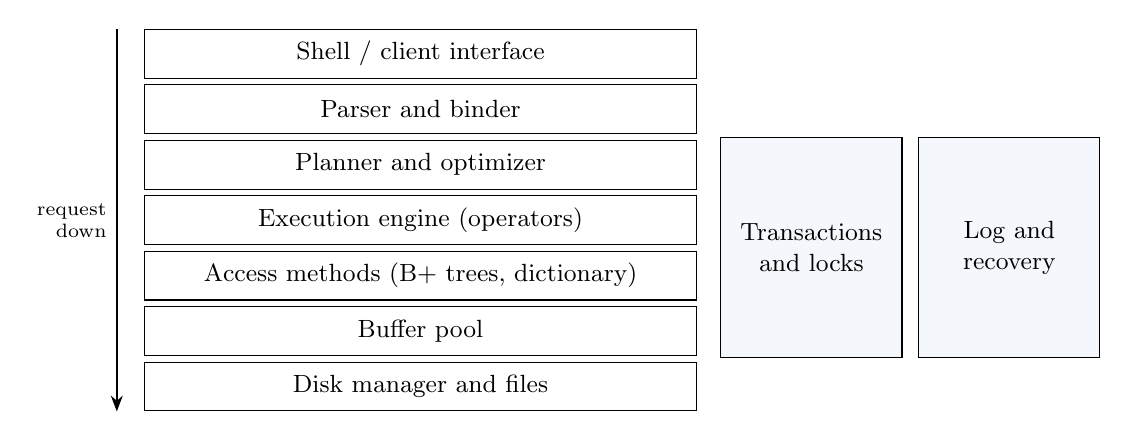
\begin{tikzpicture}[layer/.style={draw,minimum width=7cm,minimum height=0.62cm,font=\small,fill=white},
                    side/.style={draw,minimum width=2.3cm,minimum height=2.8cm,font=\small,align=center,fill=boxbg}]
\node[layer] (shell) {Shell / client interface};
\node[layer,below=2pt of shell] (parse) {Parser and binder};
\node[layer,below=2pt of parse] (plan) {Planner and optimizer};
\node[layer,below=2pt of plan] (exec) {Execution engine (operators)};
\node[layer,below=2pt of exec] (access) {Access methods (B+ trees, dictionary)};
\node[layer,below=2pt of access] (bpm) {Buffer pool};
\node[layer,below=2pt of bpm] (disk) {Disk manager and files};
\node[side,right=0.3cm of exec,yshift=-0.35cm] (txn) {Transactions\\and locks};
\node[side,right=0.2cm of txn] (log) {Log and\\recovery};
\draw[arrow] ([xshift=-0.35cm]shell.north west) -- node[left,font=\scriptsize,align=right]{request\\down} ([xshift=-0.35cm]disk.south west);
\end{tikzpicture}
\caption{The layers of a database engine. Transactions and recovery cut across the stack.}
\label{fig:layers}
\end{figure}

\begin{description}[leftmargin=1.2em]
\item[Interface] Reads text, returns results. For OntoDB this is the \code{ontodb} shell.
\item[Parser and binder] Turn text into a tree, check names, and replace each constant with an internal id.
\item[Planner and optimizer] Choose \emph{how} to answer: which index to use, in what order to join, with which algorithm.
\item[Execution engine] Runs the chosen plan as a tree of operators that pass rows to each other.
\item[Access methods] The data structures that find data: B+ trees for ranges, hash tables for exact matches, the dictionary for term ids.
\item[Buffer pool] Caches disk pages in memory, decides which to evict, and enforces the write-ahead rule when a page goes back to disk.
\item[Disk manager] Reads and writes fixed-size pages of a file.
\end{description}

Two subsystems do not fit in one layer. The \textbf{transaction manager} and
\textbf{lock manager} touch every read and write. The \textbf{log manager}
and \textbf{recovery} touch every update, every page write, and every restart.
Most of the difficulty of building an engine lives in how these cross-cutting
pieces interact with the layers.

\begin{keyidea}
Each layer hides a cost from the one above. The buffer pool hides the disk; the
B+ tree hides how many pages a lookup needs; the optimizer hides that a query
can be answered in a thousand ways. Understanding an engine means knowing what
each layer hides, and when the hiding fails.
\end{keyidea}

\section{RDF in one page}

RDF represents knowledge as a set of \term{triples}. A triple is
\emph{(subject, predicate, object)}: the subject is a thing, the predicate a
relationship, and the object another thing or a value.

\begin{lstlisting}
<http://ex.org/Alice>  <http://ex.org/name>       "Alice"
<http://ex.org/Alice>  rdf:type                   <http://ex.org/Student>
<http://ex.org/Metal>  rdfs:subClassOf            <http://ex.org/Material>
\end{lstlisting}

Things are named by IRIs (\code{<http://...>}); values are literals, optionally
with a language (\code{"Métal"@fr}) or a datatype (\code{"21"\^{}\^{}xsd:integer}).
An \term{ontology} is RDF that describes concepts and their relations:
\code{Metal subClassOf Material}, \code{Alloy subClassOf Metal}. OWL, the
standard ontology language, is itself written as RDF triples, so a triple store
can store any OWL ontology without understanding it.

\section{SPARQL in one page}

SPARQL asks questions by \emph{pattern}. A \term{triple pattern} is a triple in
which some positions are variables. A \term{basic graph pattern} is a set of
triple patterns that share variables; its answers are every way of binding the
variables so that every pattern becomes a stored triple.

\begin{lstlisting}
PREFIX ub: <http://example.edu/univ#>
SELECT ?name WHERE {
  ?s a ub:Student .        # ?s is a student
  ?s ub:name ?name .       # ... and has a name
}
\end{lstlisting}

Two patterns that share \code{?s} are a \emph{join}. That is the single most
important fact about evaluating SPARQL: a query with $k$ patterns is a $k$-way
self-join of one large table of triples. Everything in \cref{ch:rdf-indexing}
and \cref{ch:joins} follows from it.

\section{The running example}

\begin{ontodb}
OntoDB is a database management system for ontologies, written in C++20. It
loads Turtle, N-Triples, and RDF/XML (so OWL files load as triples), and it
answers SPARQL basic graph patterns with filters, \code{INSERT DATA}, and
\code{DELETE DATA}. Its layers map one to one onto \cref{fig:layers}:
a shell (\code{tools/shell}), a lexer, parser, and binder (\code{src/parser},
\code{src/binder}), a planner and optimizer, volcano executors
(\code{src/execution}), a dictionary and a store (\code{src/dictionary},
\code{src/store}), a buffer pool and disk manager (\code{src/buffer},
\code{src/storage}), and a log and recovery manager (\code{src/recovery}).
\end{ontodb}

A single query, followed through OntoDB, touches every layer:

\begin{enumerate}
\item The shell reads lines until the query's braces balance.
\item The parser builds a syntax tree; the binder resolves prefixes, turns every IRI and literal into a 64-bit id from the dictionary, and gives each variable a column number.
\item The planner builds a tree: one scan per triple pattern, joins between them, a filter, a projection.
\item The execution engine pulls rows of ids up that tree, one at a time.
\item The shell turns ids back into text through the dictionary and prints them.
\end{enumerate}

An insert adds a sixth step: before the shell says \code{inserted 1 triple},
a log record describing the insert must be on disk. Why that order is
non-negotiable, and how it lets the engine survive a crash, is the subject of
\cref{part:recovery-ref}. First, storage.


\part{Storage}
\chapter{Disks, Files, and Pages}
\label{ch:pages}

Every design decision in a storage engine starts from one fact: memory is fast
and volatile, and storage is slow and durable. A database must keep its data on
the slow, durable device and still answer queries at the speed of the fast,
volatile one. This chapter is about the unit that moves between the two: the
\term{page}.

\section{The storage hierarchy}

\begin{table}[ht]
\centering
\begin{tabular}{@{}lll@{}}
\toprule
Device & Typical access latency & Survives power loss \\
\midrule
CPU cache & 1--10 ns & no \\
Main memory (DRAM) & about 100 ns & no \\
NVMe SSD, random 4 KiB read & 10--100 $\mu$s & yes \\
Spinning disk, random read & 5--10 ms & yes \\
\bottomrule
\end{tabular}
\caption{Orders of magnitude, not benchmarks. The gap between memory and storage is a factor of a hundred to a hundred thousand.}
\label{tab:hierarchy}
\end{table}

Two properties of storage shape everything above it.

\begin{description}[leftmargin=1.2em]
\item[Block granularity.] A device reads and writes whole blocks (typically 512 bytes or 4 KiB). Reading one byte costs a whole block. So the engine should arrange data so that one block read brings many useful bytes.
\item[Sequential beats random.] Even on SSDs, sequential access is cheaper than random access, and on spinning disks it is dramatically cheaper. An engine that writes sequentially (a log) and reads mostly through an index (a tree) uses the device the way it wants to be used.
\end{description}

\section{Pages}

A \term{page} is the engine's unit of I/O: a fixed-size block of the database
file, usually 4, 8, or 16 KiB, aligned to the device's block size. The engine
never reads half a page and never writes half a page. Fixing the size has three
payoffs:

\begin{itemize}
\item \textbf{Addressing is arithmetic.} Page $i$ lives at byte offset $i \times \text{PAGE\_SIZE}$ in the file. A page id is all the engine needs to find it.
\item \textbf{Memory is interchangeable.} Every buffer-pool frame holds exactly one page, so any frame can hold any page (\cref{ch:buffer}).
\item \textbf{Failure is bounded.} A write either lands a whole page, or, if power fails mid-write, produces a \term{torn page}: part old, part new. Because the size is fixed and known, a checksum over the page detects the tear.
\end{itemize}

\begin{keyidea}
A page id is a stable name. Pointers inside the database (a B+ tree child, a
heap record's location) are page ids, never memory addresses, so they remain
valid across restarts and across evictions.
\end{keyidea}

\section{Slotted pages}

Fixed-size records are easy to place: record $k$ starts at byte $k \times
\text{size}$. Real data is variable-sized: an IRI might be 20 bytes or 200.
The standard answer is the \term{slotted page}.

\begin{figure}[ht]
\centering
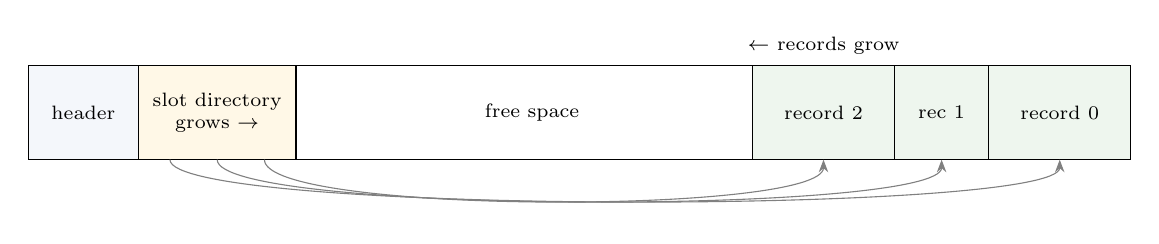
\begin{tikzpicture}[x=1cm,y=1cm,font=\scriptsize]
\fill[boxbg] (0,0) rectangle (1.4,1.2); \node at (0.7,0.6) {header};
\fill[ideabg] (1.4,0) rectangle (3.4,1.2); \node[align=center] at (2.4,0.6) {slot directory\\grows $\rightarrow$};
\node at (6.4,0.6) {free space};
\fill[statusbg] (9.2,0) rectangle (11.0,1.2); \node at (10.1,0.6) {record 2};
\fill[statusbg] (11.0,0) rectangle (12.2,1.2); \node at (11.6,0.6) {rec 1};
\fill[statusbg] (12.2,0) rectangle (14,1.2); \node at (13.1,0.6) {record 0};
\draw (9.2,0) -- (9.2,1.2); \draw (11.0,0) -- (11.0,1.2); \draw (12.2,0) -- (12.2,1.2);
\draw (1.4,0) -- (1.4,1.2); \draw (3.4,0) -- (3.4,1.2);
\draw (0,0) rectangle (14,1.2);
\node at (10.1,1.45) {$\leftarrow$ records grow};
\foreach \sx/\tx in {1.8/13.1,2.4/11.6,3.0/10.1}{\draw[-{Stealth[length=1.6mm]},gray] (\sx,0) .. controls (\sx,-0.7) and (\tx,-0.7) .. (\tx,0);}
\end{tikzpicture}
\caption{A slotted page. The slot directory grows forward from the header, records grow backward from the end, and free space sits between them.}
\label{fig:slotted}
\end{figure}

The header records how many slots exist and where free space begins. Each slot
holds a record's offset and length. A record is addressed by a \term{record id}
(RID): \emph{(page id, slot number)}. Two properties make this work:

\begin{itemize}
\item \textbf{Records can move without changing their RID.} To compact the page, slide records together and update the slot offsets. The slot number, and therefore the RID, is unchanged.
\item \textbf{Deletion is cheap.} Mark the slot free; a later insert may reuse it. The space is reclaimed when the page is compacted, or when a new record fits in the hole.
\end{itemize}

\begin{ontodb}[: pages and the term heap]
Every OntoDB page is 4096 bytes (\code{PAGE\_SIZE}). The first 8 bytes of
\emph{every} page, from the very first version, are reserved for the
\term{pageLSN}, the log sequence number of the last update applied to that
page; the payload starts at byte 8. Reserving the field before any logging
existed means the file format did not have to change when the write-ahead log
arrived (\cref{ch:wal}).

The spellings of IRIs and literals live in a \term{term heap} made of slotted
pages. The B+ tree leaves never contain strings: they contain 24-byte keys of
three ids. That separation keeps the tree's fanout high, and it is why a long
IRI costs nothing in the index (\cref{ch:rdf-indexing}). A spelling is never
deleted when a triple using it is deleted: the dictionary keeps the id, so a
log record written earlier can still name it.
\end{ontodb}

\section{Talking to the file system}

An engine reads and writes its file through the operating system, and two
details of that conversation decide whether data survives a crash.

\paragraph{The page cache.} A \code{write} call returns as soon as the bytes are
in the operating system's page cache, in memory. They reach the device later.
A crash after \code{write} returns can still lose them.

\paragraph{\code{fsync}.} Calling \code{fsync} on a file asks the operating
system to push that file's dirty data to the device and wait until the device
reports it durable. It is the only promise of durability the engine gets, and
it is expensive: a few milliseconds on a disk, tens to hundreds of microseconds
on an SSD. Two consequences follow.

\begin{enumerate}
\item \textbf{Batch the expensive call.} Engines amortize \code{fsync} across many transactions; the log manager's \term{group commit} (\cref{ch:wal}) exists for this.
\item \textbf{Never assume a failed \code{fsync} can be retried.} On several operating systems, after \code{fsync} reports an error the kernel may already have discarded the dirty pages and cleared the error, so a second \code{fsync} that ``succeeds'' has lost data. PostgreSQL learned this in 2018 and now treats a failed \code{fsync} as fatal \cite{fsyncgate,pillai2014}.
\end{enumerate}

\paragraph{Atomic replacement.} Renaming a file over another is atomic on POSIX
file systems: a reader sees the old file or the new one, never a mixture. The
idiom ``write to a temporary file, \code{fsync} it, \code{rename} it over the
target, \code{fsync} the directory'' replaces a whole file atomically. OntoDB
writes its snapshots this way (\cref{ch:durability}).

\begin{decision}{4 KiB pages}
\dpart{Choice} \code{PAGE\_SIZE} is 4096 bytes, fixed for the whole system.
\dpart{Alternatives} 8 KiB (PostgreSQL), 16 KiB (InnoDB), or a size chosen per
database at creation.
\dpart{Why} 4 KiB matches the operating system's page and a common device
block, so one page is one block. It is also small enough that tests with a
pool of three or four frames, and trees of a few hundred keys, exercise
eviction, splits, and merges quickly.
\dpart{Cost} Lower fanout than a 16 KiB page, so a very large index may need
one more level; and fixed per-page overhead (the 8-byte pageLSN, the header) is
a larger share of each page.
\end{decision}

\begin{decision}{Page 0 is a real page}
\dpart{Choice} Page ids are \code{int32}, and page 0 is a legal page.
``No page'' is \code{INVALID\_PAGE\_ID}, which is $-1$. The catalog (plan 3.3) will
initialize its page explicitly, so a zero-filled file cannot be read as ``the root is page
0''.
\dpart{Alternatives} Reserve page 0 as a null page and use 0 as the sentinel.
\dpart{Why} Zero is the value memory and files have by accident. A sentinel
should be a value that never appears unless someone wrote it on purpose; then a
missing initialization is a visible error, not a tree rooted at page 0.
\dpart{Cost} Every reader of a stored page id must check for $-1$, and the
largest file is $2^{31}$ pages, 8 TiB at 4 KiB.
\end{decision}

\begin{decision}{The file's length records allocation}
\dpart{Choice} \code{AllocatePage} grows the database file by one zero page
(\code{ftruncate}, which usually writes no data blocks). On open, the number of
allocated pages is the file size divided by \code{PAGE\_SIZE}, rounded up. There
is no header page of the disk manager's own.
\dpart{Alternatives} A header page (a superblock) holding the next page id and
a free list, as SQLite's first page and InnoDB's space header do.
\dpart{Why} Page 0 already belongs to the catalog. The file system updates a
file's length as one fact, so there is no second record of allocation that a
crash could leave disagreeing with the file.
\dpart{Cost} The new length is durable only after an \code{fsync}, so after a
crash a page that a log record names may lie past the end of the file. The disk
manager therefore reads any page past the end as zeros and grows the file when
one is written there, which lets redo apply such a record with no special case.
\end{decision}

\begin{decision}{The file only grows}
\dpart{Choice} \code{DeallocatePage} does not return the id for reuse. A freed
page stays in the file, unused.
\dpart{Alternatives} An in-memory free list, or a durable free-space map such
as PostgreSQL's.
\dpart{Why} An id that is reused while anything still names it (a log record
awaiting redo, a stale parent pointer after a crash) turns an old reference
into a write to someone else's page. It is the same argument as for term ids:
an id's meaning should not change.
\dpart{Cost} Space freed by merges and deletes is not reclaimed. Reclaiming it
safely needs a logged free-space map, which is later work.
\end{decision}

\begin{decision}{Through the page cache; \code{fsync} at shutdown}
\dpart{Choice} Pages are read and written with \code{pread} and \code{pwrite}
through the operating system's page cache. \code{WritePage} does not
\code{fsync}; \code{ShutDown} does, once.
\dpart{Alternatives} \code{O\_DIRECT}, bypassing the page cache as InnoDB can;
or \code{fsync} after every page write.
\dpart{Why} Durability is the log's job: a committed change survives because
its log record is forced (\cref{ch:wal}), not because its page is. A page needs
to be on disk only at a checkpoint or a clean shutdown. \code{pread} and
\code{pwrite} carry their own offset, so threads share one file descriptor
without a lock around a seek.
\dpart{Cost} A cached page exists twice, in a pool frame and in the kernel's
cache. Until page-level logging exists (plan 8.3), only a clean shutdown makes
the page store durable.
\end{decision}

\begin{decision}{Spellings are never deleted}
\dpart{Choice} Deleting the last triple that uses a term keeps the term and its
id in the dictionary.
\dpart{Alternatives} Reference-count terms and reclaim an id when its count
reaches zero; or garbage-collect unused terms at checkpoint.
\dpart{Why} Log records name terms by id. If id 18 could be reclaimed and
reused, an old record that says ``insert (18, 9, 4)'' would silently mean a
different triple on replay. Never deleting makes an id's meaning permanent.
\dpart{Cost} The dictionary only grows. A workload that churns through unique
literals keeps every one of them.
\end{decision}

\begin{status}
The page frame and the pageLSN layout exist, and the disk manager runs (plan
1.1): it allocates pages by growing the file, reads and writes whole pages, and
fsyncs on shutdown. The term heap is plan 3.1.
\end{status}

\begin{checkyourself}
\item Page 37 of a 4 KiB-page file: at what byte offset does it start, and why does the engine never need a table to find it?
\item In a slotted page, a record is moved during compaction. Why does no index entry that points to it need to change?
\item A \code{write} returned successfully and then the machine lost power. Was the data durable? What call would have made it so?
\item \code{fsync} returns an error. Why is calling it again and continuing on success wrong?
\item Why is $-1$ a better ``no page'' sentinel than 0?
\item After a crash, a log record names page 812, but the file holds only 800 pages. How can OntoDB's allocation scheme produce this, and who must repair it?
\end{checkyourself}

\section*{Further reading}
Petrov \cite{petrov}, chapters 2 and 3, on file formats and slotted pages.
Pillai et al.\ \cite{pillai2014} on what file systems actually guarantee.

\chapter{The Buffer Pool}
\label{ch:buffer}

The database is larger than memory, but queries must run at memory speed. The
\term{buffer pool} bridges the two: a fixed array of in-memory \term{frames},
each able to hold one page, plus the bookkeeping that decides which pages are
in memory and when they go back to disk.

\section{Frames, the page table, and pins}

\begin{figure}[ht]
\centering
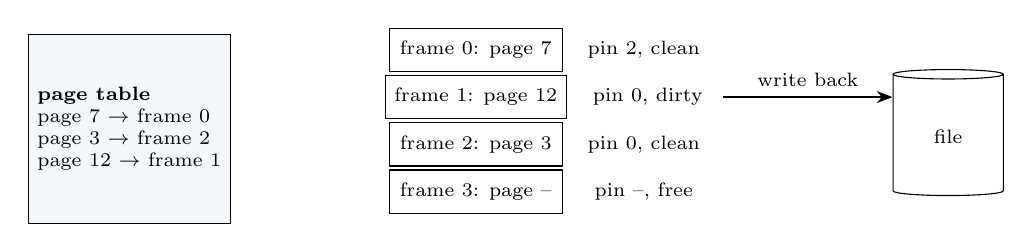
\begin{tikzpicture}[font=\scriptsize]
\node[draw,minimum width=2.4cm,minimum height=2.4cm,align=left,fill=boxbg] (pt) {\textbf{page table}\\page 7 $\to$ frame 0\\page 3 $\to$ frame 2\\page 12 $\to$ frame 1};
\foreach \i/\p/\pin/\d in {0/7/2/clean,1/12/0/dirty,2/3/0/clean,3/--/--/free}{
  \node[draw,minimum width=2.2cm,minimum height=0.55cm,fill=white] (f\i) at (4.4,1.0-0.6*\i) {frame \i: page \p};
  \node[right=2pt of f\i,align=left,minimum width=1.9cm] (s\i) {pin \pin, \d};
}
\node[draw,cylinder,shape border rotate=90,aspect=0.2,minimum height=1.6cm,minimum width=1.4cm,fill=white] (disk) at (10.4,-0.1) {file};
\draw[arrow] (s1.east) -- node[above]{write back} (disk.west |- s1.east);
\end{tikzpicture}
\caption{A buffer pool with four frames. The page table maps page ids to frames; each frame has a pin count and a dirty bit.}
\label{fig:bpm}
\end{figure}

Each frame carries two pieces of state:

\begin{description}[leftmargin=1.2em]
\item[Pin count.] How many threads are using the page right now. A pinned page must not be evicted: someone holds a pointer into it.
\item[Dirty bit.] Whether the in-memory copy differs from the one on disk. A dirty page must be written before its frame is reused.
\end{description}

The interface follows from that:

\begin{itemize}
\item \code{FetchPage(id)}: if the page is in a frame, increment its pin and return it (a \term{hit}); otherwise choose a victim frame, write it back if dirty, read the page into it, pin it (a \term{miss}).
\item \code{UnpinPage(id, dirty)}: decrement the pin; mark the frame dirty if the caller changed it.
\item \code{NewPage()}: allocate a page id on disk and return a zeroed, pinned frame.
\item \code{FlushPage(id)}: write a dirty page now.
\end{itemize}

\begin{keyidea}
A pin is a promise, and a leaked pin is a leak of memory the pool can never
reclaim. Engines therefore wrap pins in a scoped object (a \term{page guard})
that unpins exactly once when it goes out of scope.
\end{keyidea}

\section{Choosing a victim}

When every frame is occupied and a miss arrives, the pool must evict an
unpinned page. The choice matters: a bad policy turns hits into misses, and
every miss is a disk read.

\paragraph{LRU.} Evict the least recently used page. Simple, and good for many
workloads. Its weakness is \term{sequential flooding}: one large scan touches
every page once, and each touch makes a cold scan page look ``recent'', so the
scan flushes out the hot index pages that every other query needs.

\paragraph{CLOCK.} An approximation of LRU that avoids moving pages in a list on
every access: each frame has a reference bit set on access, and a ``clock hand''
sweeps the frames, clearing bits and evicting the first frame whose bit is
already clear. Cheap, and still vulnerable to flooding.

\paragraph{LRU-K.} O'Neil, O'Neil, and Weikum's fix for flooding \cite{lruk}.
Remember the last $K$ access times of each page. The \term{backward
$K$-distance} of a page is the time since its $K$-th most recent access; a page
accessed fewer than $K$ times has infinite distance. Evict the page with the
largest distance.

With $K=2$, a page touched once by a scan has infinite distance, while an index
root touched thousands of times has a small one. The scan page goes first. LRU
is the special case $K = 1$.

\begin{table}[ht]
\centering
\begin{tabular}{@{}lccc@{}}
\toprule
Page & Accesses (time) & 2nd most recent & Backward 2-distance at $t=10$ \\
\midrule
A (index root) & 1, 4, 8, 9 & 8 & 2 \\
B (index leaf) & 3, 6 & 3 & 7 \\
C (scanned once) & 7 & --- & $\infty$ \\
\bottomrule
\end{tabular}
\caption{LRU-K with $K=2$. LRU would evict B (least recently used at time 6); LRU-K evicts C, the page with no second access, even though C was touched more recently than B.}
\label{tab:lruk}
\end{table}

When several pages have infinite distance, a tie-breaking rule is needed.
A common choice is the page whose oldest remembered access is earliest; with
$K = 2$ such a page has exactly one access, so this is plain LRU among the
pages seen once.

\section{Steal and force}

Two policy questions connect the buffer pool to recovery, and their answers
decide what the log must contain.

\begin{description}[leftmargin=1.2em]
\item[Steal?] May the pool write a dirty page of an \emph{uncommitted} transaction to disk, to free its frame? If yes, the disk can hold changes that must later be \emph{undone}.
\item[Force?] Must every page a transaction changed be written to disk \emph{before} it commits? If no, a committed change may exist only in memory at the time of a crash, and must later be \emph{redone}.
\end{description}

\begin{table}[ht]
\centering
\begin{tabular}{@{}lll@{}}
\toprule
& Force & No force \\
\midrule
No steal & no undo, no redo (slow, memory-bound) & redo only \\
Steal & undo only & undo and redo (fast, flexible) \\
\bottomrule
\end{tabular}
\caption{The four combinations. High-performance engines choose steal and no force, and pay for it with a log that supports both undo and redo.}
\label{tab:stealforce}
\end{table}

Steal lets the pool evict any unpinned page, so a long transaction cannot
exhaust memory. No force lets a commit write one small log record instead of
every page it touched. Both are wins, and \cref{ch:wal,ch:aries} show how the
log makes them safe.

\begin{ontodb}[: the buffer pool]
OntoDB's pool uses \textbf{LRU-K} with $K = 2$ by default (\code{\textbackslash set lru\_k}),
tie-breaking by the older $K$-th access. Its policy is \textbf{steal / no force}.
Pages are reached only through \code{ReadPageGuard} (shared latch, one pin)
and \code{WritePageGuard} (exclusive latch, one pin); both unpin exactly once.
The test harness asserts that the number of pinned frames is zero after every
query and every destroyed iterator: a leaked pin fails the test even when the
query's rows were right.

When the pool writes a dirty page and a log manager is installed, the order is
fixed: first flush the log up to the page's pageLSN, then write the page. A
named crash point sits between the two, so a test can kill the process after the
log is durable and before the page is. That ordering is the write-ahead rule of
\cref{ch:wal}.
\end{ontodb}

\begin{decision}{One I/O thread, first in, first out}
\dpart{Choice} The pool never calls the disk manager itself. It hands a request
to a \code{DiskScheduler}, whose single background thread runs reads and writes
in the order they were scheduled. \code{Schedule} returns at once with a
future; if the I/O fails, the error is rethrown from the future's \code{get}.
\dpart{Alternatives} Synchronous I/O on the query thread; a pool of I/O
threads; an asynchronous kernel interface such as \code{io\_uring}.
\dpart{Why} In-order execution makes ``write page 9, then read page 9'' correct
with no per-page bookkeeping. A background thread lets a flush or a prefetch
overlap with query work, and errors arrive where the waiting caller can handle
them.
\dpart{Cost} No parallel I/O: an SSD reaches full throughput only with many
requests in flight, and one slow read delays every request behind it.
\end{decision}

\begin{decision}{LRU-K with $K = 2$}
\dpart{Choice} Evict the unpinned frame with the largest backward 2-distance.
Frames seen fewer than twice have infinite distance and go first, earliest
oldest access first. Time is a logical clock that ticks on every access, not
the wall clock, and a pinned frame keeps its history.
\dpart{Alternatives} LRU, CLOCK, 2Q, ARC.
\dpart{Why} SPARQL plans scan: an unselective pattern reads every leaf of a
permutation once. LRU and CLOCK let that scan push out the index's upper levels;
LRU-K does not. A logical clock and a fixed tie-break make eviction
deterministic, so a test can predict exactly which frame goes; the replacer's
tests replay \cref{tab:lruk} and check that C, not B, is evicted. Keeping
history while a frame is pinned stops a hot page from looking new each time it
is unpinned.
\dpart{Cost} Each frame keeps $K$ timestamps, and choosing a victim scans every
frame: linear in the pool size, which is cheap for the default 64 frames but
would need a priority structure for pools of millions. A second policy is
planned as a measured comparison, not as a replacement.
\end{decision}

\begin{decision}{One latch for the whole pool, held across I/O}
\dpart{Choice} A single mutex covers the page table, the free list, every pin
count and dirty bit, and the replacer calls. It stays held while a miss reads
its page or a victim is written back.
\dpart{Alternatives} Partition the page table and give each frame an
``I/O in progress'' state, so other threads keep working during a read; this is
roughly what PostgreSQL does with buffer-mapping partitions and per-buffer I/O
locks.
\dpart{Why} The pool's state is then always consistent: no frame is
half-loaded while another thread looks it up, and the tests pass under
ThreadSanitizer without subtle protocols. With a single I/O thread
(design decision on the scheduler), finer locking would mostly move the
waiting elsewhere.
\dpart{Cost} A miss stalls every thread for one disk read. Finer-grained
latching is the first thing to change when I/O becomes parallel.
\end{decision}

\begin{decision}{The pool's destructor does not flush}
\dpart{Choice} Destroying the pool discards dirty frames. Durable shutdown
calls \code{FlushAllPages} explicitly (plan 3.6).
\dpart{Alternatives} Flush every dirty page on destruction, which is
convenient.
\dpart{Why} Durability is the log's job. Tests need a path that behaves like a
dead process, writing nothing, and a destructor also runs while an exception
from a crash point unwinds; a flushing destructor would write exactly the page
the test is trying to keep off disk.
\dpart{Cost} A caller who forgets \code{FlushAllPages} loses work on a clean
exit. The clean-restart test of plan 3.6 is there to catch it.
\end{decision}

\begin{decision}{A full pool returns null}
\dpart{Choice} When every frame is pinned, \code{NewPage} and
\code{FetchPage} return \code{nullptr} at once.
\dpart{Alternatives} Block until some frame is unpinned, or throw.
\dpart{Why} The caller usually holds pins of its own; blocking could wait for
a pin that only the waiter can release. Returning lets the caller give up the
operation and release what it holds.
\dpart{Cost} Every caller must check for null; guards and the tree turn that
into an error close to the cause.
\end{decision}

\begin{decision}{Pages only through guards}
\dpart{Choice} Code above the pool reaches a page only through a
\code{ReadPageGuard} or \code{WritePageGuard}: one pin plus a latch, released
exactly once by \code{Drop} or the destructor. Guards move but never copy, and a
moved-from guard is empty. Tests assert the pinned-frame count is zero after
every query.
\dpart{Alternatives} Callers call \code{UnpinPage} by hand, as early textbook
pools do.
\dpart{Why} A leaked pin returns the right rows and silently shrinks the pool;
a double unpin lets a page in use be evicted. Neither is visible in query
results. Tying the pin to a scope removes both.
\dpart{Cost} Ownership rules (move-only, drop before pinning the sibling) that
every caller must follow, and a little ceremony for one-line accesses.
\end{decision}

\begin{decision}{Pin, then latch; unlatch, then unpin}
\dpart{Choice} Each frame has a reader--writer latch. A guard asks the pool to
pin the page, then takes the latch, outside the pool's own latch. Dropping
releases the latch first and the pin second. A null page from the pool becomes
an error at the call that asked for it.
\dpart{Alternatives} Take the page latch while still holding the pool latch;
or release the pin before the latch.
\dpart{Why} Waiting for a page latch while holding the pool latch would block
every thread behind one busy page, and could deadlock with the thread that
holds the page and needs the pool. Unpinning first would let the frame be
evicted and reused while its latch is still held.
\dpart{Cost} Between the pin and the latch, another writer may get the page
first; callers must not assume what they will find.
\end{decision}

\begin{decision}{A latch belongs to a page, not to a frame}
\dpart{Choice} When a frame is given to a different page, it gets a new latch.
This happens only while the frame is unpinned, and since guards pin before they
latch, no thread holds or waits on the old one.
\dpart{Alternatives} One latch per frame for the life of the pool.
\dpart{Why} Latch order is a rule about pages: top-down and left to right. With
a latch per frame, two unrelated pages that once shared a frame look like the
same lock, and ThreadSanitizer reported a lock-order cycle in a bulk load on a
three-frame pool that could never deadlock. A fresh latch makes the checker see
the same thing the protocol is about.
\dpart{Cost} A small allocation on every page load, next to a disk read that
costs far more. (It has to be a new allocation: ThreadSanitizer forgets a mutex
when its memory is freed, but not when a statically initialized
\code{std::shared\_mutex} is destroyed and rebuilt in place, which was the first
attempt.)
\end{decision}

\begin{decision}{A write guard dirties only if written}
\dpart{Choice} A write guard marks the page dirty on drop only if its mutable
\code{GetData} was called.
\dpart{Alternatives} Every write guard marks its page dirty.
\dpart{Why} B+ tree latch crabbing takes exclusive latches on pages it may
never change. Marking those dirty would write clean pages back to disk.
\dpart{Cost} Code that writes through a pointer obtained earlier, after
dropping the guard, escapes the dirty bit, which is one more reason never to
keep that pointer.
\end{decision}

\begin{decision}{Inspecting a page goes through the pool}
\dpart{Choice} \code{\textbackslash page N} reads page $N$ with a read guard,
as any operator would, and prints its pageLSN and the first payload bytes.
\code{\textbackslash bpm} prints each frame's page, pins, dirty bit, and
pageLSN.
\dpart{Alternatives} Read the page straight from the file, bypassing the pool.
\dpart{Why} The pool's copy is what the engine sees, including changes that
are dirty and not yet on disk. Reading the file would show a page the engine
has already moved past.
\dpart{Cost} Looking is an access: it can load the page, evict another, and add
to the page's LRU-K history. The observer changes what it observes, so
\code{\textbackslash bpm} is best read before \code{\textbackslash page}.
\end{decision}

\begin{status}
The disk manager, the I/O scheduler, the LRU-K replacer, and the pool run
(plans 1.1 to 1.4), and so do page guards with per-frame reader--writer latches
(plan 1.5) and the shell's \code{\textbackslash bpm}, \code{\textbackslash page},
and \code{\textbackslash trace} (plan 1.6): the buffer pool is complete. It
already flushes the log up to a page's pageLSN before writing the page. The
default memory backend has no pool, so these commands come alive with the
indexed store (plan 3.4).
The experiment that checks them is simple: run a scan with a pool of 4 frames
and of 64, with $K=1$ and $K=2$, and compare hits and misses in \code{\textbackslash stats}.
\end{status}

\begin{checkyourself}
\item A frame has pin count 0 and is dirty. What must happen before a different page is read into it?
\item In \cref{tab:lruk}, add an access to C at time 10. Which page does LRU-K evict at time 11 now?
\item With $K = 3$, frame X has accesses at times 2 and 9, and frame Y only at time 5. Both are unpinned. Which does OntoDB evict, and why is X's more recent access irrelevant?
\item Explain sequential flooding, and why $K = 2$ resists it while $K = 1$ does not.
\item Which cell of the steal/force table needs \emph{undo} information in the log, and why?
\item A thread schedules a write of page 9 and then, without waiting, a read of page 9 into another buffer. What does the read return in OntoDB, and what could go wrong with a pool of I/O threads?
\item Two threads miss on two different pages at the same moment. In OntoDB's pool, how long does the second thread wait, and why?
\item A test arms the crash point between the log flush and the page write, and the exception unwinds through the pool's destructor. Why would a destructor that flushes dirty pages ruin the test?
\item Why does a guard release its latch \emph{before} it unpins the page, and not after?
\item You run \code{\textbackslash page 7} twice and then \code{\textbackslash bpm}. How has inspecting the page changed the pool?
\item A query returns the right rows, but afterwards one frame is still pinned. What will go wrong later, and how do OntoDB's guards prevent it?
\end{checkyourself}

\section*{Further reading}
Petrov \cite{petrov}, chapter 5 on buffer management. O'Neil et al.\ \cite{lruk}.
Effelsberg and H\"arder \cite{effelsberg} on buffer management principles.

\chapter{B-Trees and B+ Trees}
\label{ch:btree}

An index answers ``where is the data with this key?'' without reading all the
data. For data on disk the answer has been the same since 1970: the B-tree of
Bayer and McCreight \cite{bayer1972}, and its variant the B+ tree, described by
Comer as ubiquitous \cite{comer1979}. This chapter explains why it fits disks so
well, and how it stays balanced.

\section{Why a tree of pages}

A binary search tree has fanout 2: each node has two children, so finding one
of $N$ keys takes about $\log_2 N$ steps. If every step is a page read, a
billion keys need 30 reads. A B-tree makes each node a whole \emph{page} and
packs as many keys into it as fit. With fanout $F$, a lookup takes
$\log_F N$ reads.

\begin{table}[ht]
\centering
\begin{tabular}{@{}rrr@{}}
\toprule
Fanout $F$ & Height for $10^9$ keys & Height for $10^{12}$ keys \\
\midrule
2 & 30 & 40 \\
100 & 5 & 6 \\
500 & 4 & 5 \\
\bottomrule
\end{tabular}
\caption{Height is $\lceil\log_F N\rceil$. A large fanout turns a billion-key lookup into four page reads, and the top levels are almost always in the buffer pool.}
\end{table}

The upper levels are tiny (a tree of fanout 500 has 1 root and 500 children
above a quarter-million leaves) and hot, so they stay in the buffer pool. In
practice a lookup costs one or two actual disk reads.

\begin{keyidea}
A B-tree is a binary search tree redesigned for block devices: make each node a
page, make the fanout as large as the page allows, and the tree is shallow
enough that its top fits in memory.
\end{keyidea}

\section{B-tree versus B+ tree}

A \term{B-tree} stores keys and values in every node. A \term{B+ tree} stores
values only in the \term{leaves}; internal nodes hold only \term{separator keys}
that direct the search. Two consequences favor the B+ tree for databases:

\begin{itemize}
\item \textbf{Higher fanout.} Internal nodes hold no values, so more separators fit per page and the tree is shallower.
\item \textbf{Fast range scans.} Leaves are linked to their right sibling. A range query finds its first key with one descent, then walks sideways along the leaf chain without climbing back up.
\end{itemize}

\begin{figure}[ht]
\centering
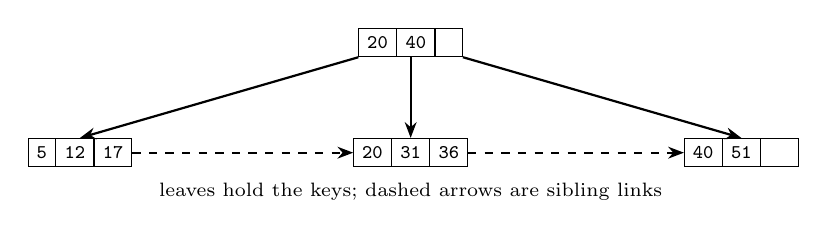
\begin{tikzpicture}[font=\scriptsize]
\node[node box=3] (root) at (0,0) {\nodepart{one}20\nodepart{two}40\nodepart{three}\phantom{0}};
\node[node box=3] (l1) at (-4.2,-1.4) {\nodepart{one}5\nodepart{two}12\nodepart{three}17};
\node[node box=3] (l2) at (0,-1.4) {\nodepart{one}20\nodepart{two}31\nodepart{three}36};
\node[node box=3] (l3) at (4.2,-1.4) {\nodepart{one}40\nodepart{two}51\nodepart{three}\phantom{00}};
\draw[arrow] (root.south west) -- (l1.north);
\draw[arrow] (root.south) -- (l2.north);
\draw[arrow] (root.south east) -- (l3.north);
\draw[arrow,dashed] (l1.east) -- (l2.west);
\draw[arrow,dashed] (l2.east) -- (l3.west);
\node[below=2pt of l2] {leaves hold the keys; dashed arrows are sibling links};
\end{tikzpicture}
\caption{A B+ tree. Keys below separator 20 are in the left child; keys from 20 up to 40 in the middle; 40 and above in the right.}
\label{fig:bptree}
\end{figure}

The \term{separator rule} is the tree's central invariant: in an internal node
with separators $k_1 < k_2 < \dots < k_n$ and children $c_0, \dots, c_n$, every
key in $c_{i-1}$ is less than $k_i$, and every key in $c_i$ is at least $k_i$.

\section{Search}

Start at the root. At each internal node, binary-search the separators to pick
the child whose range contains the key, and descend. At the leaf, binary-search
for the key. A range scan $[\ell, u)$ searches for $\ell$, then follows sibling
links until a key reaches $u$.

\section{Insertion and splits}

Insert into the leaf the search reaches. If the leaf has room, done. If it is
full, \term{split} it:

\begin{enumerate}
\item Allocate a new leaf. Move the upper half of the keys into it.
\item Link it: the new leaf's sibling is the old leaf's sibling, and the old leaf's sibling becomes the new leaf.
\item Insert a separator into the parent: the first key of the new leaf, which is \emph{copied up} (it stays in the leaf).
\item If the parent is now full, split it too. An internal split \emph{pushes up} its middle key: the key moves to the grandparent and is removed from both halves.
\item If the root splits, create a new root with two children. This is the only way the tree grows taller, so every leaf is always at the same depth.
\end{enumerate}

\begin{figure}[ht]
\centering
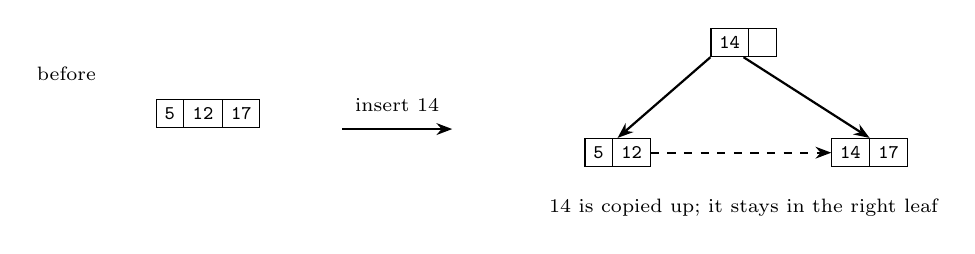
\begin{tikzpicture}[font=\scriptsize]
\node at (-5.4,0.5) {before};
\node[node box=3] (b) at (-3.6,0) {\nodepart{one}5\nodepart{two}12\nodepart{three}17};
\node at (-1.2,0.1) {insert 14};
\draw[arrow] (-1.9,-0.2) -- (-0.5,-0.2);
\node[node box=2] (p) at (3.2,0.9) {\nodepart{one}14\nodepart{two}\phantom{0}};
\node[node box=2] (a) at (1.6,-0.5) {\nodepart{one}5\nodepart{two}12};
\node[node box=2] (c) at (4.8,-0.5) {\nodepart{one}14\nodepart{two}17};
\draw[arrow] (p.south west) -- (a.north);
\draw[arrow] (p.south) -- (c.north);
\draw[arrow,dashed] (a.east) -- (c.west);
\node at (3.2,-1.2) {14 is copied up; it stays in the right leaf};
\end{tikzpicture}
\caption{A full leaf with capacity 3 splits on insert. The new right leaf's first key becomes the separator.}
\label{fig:split}
\end{figure}

A classic bug lives in step 3: if the middle key is copied up \emph{and} left in
the \emph{left} leaf, the separator rule breaks, because the right child's keys
must be at least the separator while a copy of it sits on the left. Writing an
invariant checker before writing insert catches this at once.

\section{Deletion}

Remove the key from its leaf. If the leaf is still at least half full, done.
Otherwise:

\begin{itemize}
\item \textbf{Redistribute}: if a sibling has more than half, move a key across and update the parent's separator, which must now reflect the new boundary.
\item \textbf{Merge}: otherwise combine the leaf with a sibling, remove the separator between them from the parent, and free the empty page. The parent may now underflow, and the process repeats upward; if the root is left with one child, that child becomes the root.
\end{itemize}

Many production systems relax deletion and allow underfull nodes, merging only
when a node empties: deletes are rarer than inserts, and a tree that gets a
little sparse rarely matters.

\section{Bulk loading}

Building a tree by inserting keys one at a time leaves leaves about two thirds
full and touches pages in random order. When the keys are available up front,
\term{bulk loading} is far better: sort the keys, fill leaves completely from
left to right, link them, then build each internal level from the first keys of
the level below. One sequential pass per level, and every page is full.

\section{Iterators and pins}

A range scan returns rows one at a time to the query engine, so it is an
\term{iterator} that holds a position: the current leaf and an index inside it.
The leaf must stay pinned while the iterator points into it. When the iterator
moves to the sibling, it should unpin the current leaf \emph{before} pinning the
next one; holding both, plus a parent, can exhaust a small buffer pool and
deadlock.

\begin{ontodb}[: the B+ tree]
OntoDB's index is a B+ tree. Its key is a 24-byte \code{TripleKey}
(\cref{ch:rdf-indexing}), and the leaf stores the key itself: the triple
\emph{is} the record, so there is no separate tuple id. Leaves link to their
right sibling, the header page stores the root (or \code{INVALID\_PAGE\_ID} for
an empty tree), and a scan holds no pin and no latch between rows: it copies
the rest of a leaf's keys and lets the leaf go (design decision below).

An invariant checker (\code{CheckInvariants}) verifies sizes, key order, sibling
links, and the separator rule, and the shell can draw the tree
(\code{\textbackslash tree spo dot}). Splits and merges are multi-page
operations, so they have named crash points where a recovery test may kill the
process; \cref{ch:aries} explains why a split is redone but never undone.
Bulk load sorts ids, not strings, because the tree's order is the order of the
ids.
\end{ontodb}

\begin{decision}{Fixed slots, no key compression}
\dpart{Choice} A page header of 12 bytes follows the pageLSN: type, size, and
max size. A leaf then holds its right sibling's id and an array of 24-byte keys,
169 per 4 KiB page. An internal page holds slots of a 24-byte key and a 4-byte
child id, 144 keys and 145 children per page. Every key is stored whole.
\dpart{Alternatives} Prefix compression, which stores each key as the bytes it
does not share with its neighbour (most keys in an SPO leaf share their subject),
or a slotted layout with variable-length keys.
\dpart{Why} Fixed slots make \code{KeyAt(i)} an address computation and binary
search trivial, and a key copied out of a page is complete on its own. With
fanouts above 140, a billion triples still fit in a tree of five levels.
\dpart{Cost} Keys that share a long prefix waste most of their bytes, roughly
a third of each leaf for a subject-heavy SPO index. Leaf compression is on the
list of later work, with the question of what it does to prefix bounds.
\end{decision}

\begin{decision}{The key is the record}
\dpart{Choice} A leaf stores the 24-byte \code{TripleKey} and nothing else.
There is no value field and no record id pointing to a heap.
\dpart{Alternatives} The relational layout: a heap file of tuples, with each
index mapping a key to a record id.
\dpart{Why} A triple of ids \emph{is} its whole content. A heap would store the
same 24 bytes again and cost an extra page read per match.
\dpart{Cost} Each permutation is a complete copy of the data, so the number of
permutations is a space decision (\cref{ch:rdf-indexing}).
\end{decision}

\begin{decision}{Strict deletion}
\dpart{Choice} \code{Remove} keeps every node except the root at least half
full, by redistributing from a sibling or merging with it.
\dpart{Alternatives} Lazy deletion, as many production systems do: let nodes
become sparse and free a page only when it is empty.
\dpart{Why} The invariant checker can then assert a fill factor, and merges
become real multi-page structure changes with crash points, which the recovery
chapters need.
\dpart{Cost} More page writes on delete-heavy workloads, and the most intricate
code in the tree.
\end{decision}

\begin{decision}{The invariant checker comes before insert}
\dpart{Choice} \code{CheckInvariants} (size, order, sibling links, the
separator rule) is built and tested before \code{Insert}, and every insert and
delete test runs it.
\dpart{Alternatives} Test insert by looking up the keys afterwards.
\dpart{Why} Lookups can succeed on a tree that is already wrong; the
copied-up-key bug of this chapter does exactly that. A checker turns a
structural mistake into a failure on the operation that caused it.
\dpart{Cost} Code that never runs in production paths, and a full-tree walk in
every test.
\end{decision}

\begin{decision}{Hold the path, not parent pointers}
\dpart{Choice} Pages store no pointer to their parent. An insert or delete
keeps the pages it may have to change latched on its way down (the latch
crabbing of \cref{ch:concurrency}), so a split or merge finds its parent
already in hand.
\dpart{Alternatives} A parent pointer in every page.
\dpart{Why} A split of an internal page with 145 children would have to rewrite
the parent pointer of half of them, which is dozens of page writes for one
insert. A parent pointer is also one more thing a concurrent split can make
stale.
\dpart{Cost} The latched path is pinned: an insert into a tree whose pages are
all full pins every level, so the pool must be larger than the tree's height
plus two. The first, single-threaded version remembered page ids instead and
re-read parents; that was correct only while one thread changed the tree.
\end{decision}

\begin{decision}{Split in the middle}
\dpart{Choice} A full leaf splits into two halves, and the right half's first
key is copied up. A full internal page splits around its middle key, which
moves up.
\dpart{Alternatives} Split at the insertion point when keys arrive in
increasing order, leaving the left page full, as several engines do for
append-heavy indexes.
\dpart{Why} Triples arrive in no particular order across three permutations,
and a middle split is the simplest rule that keeps every page at least half
full.
\dpart{Cost} Inserting sorted keys one at a time leaves every leaf half full,
twice the pages a scan must read. Loading sorted data is what bulk load is for.
\end{decision}

\begin{decision}{Bulk load packs leaves full}
\dpart{Choice} \code{BulkLoad} fills each leaf to its maximum, left to right,
then builds each internal level the same way. If the last node of a level would
fall below its minimum, it and its left neighbour split their entries evenly.
\dpart{Alternatives} Leave free space in each leaf, a \emph{fill factor}, as
PostgreSQL does for its B-tree indexes (90\% by default).
\dpart{Why} An ontology is loaded and then queried. Full leaves mean the fewest
pages for every scan, and loading is one sequential pass per level.
\dpart{Cost} The first insert into a full leaf splits it at once, so a tree that
is loaded and then edited heavily ends up looking like one built by inserts.
\end{decision}

\begin{decision}{A scan holds nothing between rows}
\dpart{Choice} When the iterator reaches a leaf, it copies the leaf's remaining
keys (up to the scan's upper bound), notes the right sibling's id, and releases
the leaf. It latches the sibling only when those keys run out.
\dpart{Alternatives} Keep the current leaf pinned and read-latched for as long
as the iterator sits on it, as the first version did.
\dpart{Why} A join keeps one scan open while it opens others on other trees,
so held leaf latches were taken in both orders across trees, and Linux's
ThreadSanitizer flagged the cycle. With a writer waiting between two such
readers, that is a real deadlock, and a transaction waiting for a lock while
its scan held a latch would be one the lock manager cannot see. A scan that
holds nothing cannot take part in either.
\dpart{Cost} Up to a page of keys copied per leaf. A key inserted into a leaf
after the scan copied it is not returned, and the copied keys may include one
deleted since; the scan sees each leaf as of the moment it read it, which is
what an unlocked scan promises, and transactions add locks on top.
\end{decision}

\begin{decision}{A load arrives as one batch}
\dpart{Choice} The loader parses a file (or several) completely, interning
terms as it goes, and hands the triples to the store in one call. The indexed
store, if it is empty, sorts each permutation's keys and bulk-loads every tree;
if it already holds triples, it inserts one at a time.
\dpart{Alternatives} Insert each triple as it is parsed; or rebuild the trees
from old and new keys on every load.
\dpart{Why} Measured on LUBM(1), the 15 files in one batch load in 1.1 seconds
instead of 1.7, into 10.8 MiB instead of 16.2, and every scan reads about half
the pages, because bulk load packs the leaves that random inserts left half
full. Building three trees costs barely more than one; the time left is the
dictionary's.
\dpart{Cost} A batch holds every triple of the load in memory, and only the
first load into an empty store is bulk-loaded; later loads pay for inserts and
leave half-full leaves again.
\end{decision}

\begin{decision}{Small nodes in tests}
\dpart{Choice} The tree's maximum node sizes default to what a page holds
(169 and 144 keys), and tests pass sizes as small as 2 to grow deep trees from
a few dozen keys. A randomized test inserts and deletes against a reference set
with node sizes of 2 to 5, checking every invariant after every operation.
\dpart{Alternatives} Test only with full pages, or shrink \code{PAGE\_SIZE} for
tests.
\dpart{Why} With 169 keys per leaf, a tree needs tens of thousands of keys to
reach three levels, so bugs in internal merges and root changes would hide. The
same code runs with either size; only two numbers change.
\dpart{Cost} Small nodes make some cases more common than they are in real use
and others rarer, so the full-size tests stay as well.
\end{decision}

\begin{status}
The B+ tree is complete (plans 2.1 to 2.7): the page layout, the invariant
checker and \code{ToDot}, point search, insert with splits, the prefix
iterator, bulk load, and delete with merge and redistribution, with all four
crash points. It is safe for concurrent use by latch crabbing (plan 7.1), and
the shell's \code{\textbackslash tree} draws it on the indexed backend. Loading into
an empty indexed store goes through bulk load (plan 6.1), and LUBM(1) loads and
answers queries on a 32-frame pool (plan 6.2).
\end{status}

\begin{checkyourself}
\item OntoDB's internal page has 145 slots of 28 bytes after a 20-byte header. Where do the 28 bytes come from, and why does slot 0's key go unused?
\item A page holds 300 separators. About how many levels does a tree of $10^8$ keys need, and how many of those are likely in the buffer pool?
\item During a leaf split the separator 14 is copied up. Which leaf must it stay in, and what breaks if it stays in the other one?
\item Why does an internal split \emph{push up} its middle key, while a leaf split \emph{copies} it?
\item Why should a scan unpin its current leaf before pinning the sibling?
\item Why does OntoDB not store a parent pointer in each page? What does the choice cost once several threads change the tree?
\item OntoDB bulk-loads 170 sorted keys with a leaf maximum of 169. What leaves does it build, and why not one leaf of 169 and one of 1?
\item Bulk load fills every leaf. Why can't a loop of \code{Insert} calls do the same?
\end{checkyourself}

\section*{Further reading}
Bayer and McCreight \cite{bayer1972}; Comer \cite{comer1979}; Petrov
\cite{petrov}, chapters 2, 4, and 6.

\chapter{Indexing RDF}
\label{ch:rdf-indexing}

A relational table has a schema, and each column can be indexed on its own.
An RDF store has one table with three columns, and a query can bind any subset
of them. This chapter shows how a triple store turns that into fixed-size keys
in B+ trees: first by replacing strings with integers, then by laying out the
integers so that byte order is query order, and finally by keeping more than
one ordering of the same triples.

\section{Dictionary encoding}

IRIs are long and repeated: the same predicate appears in millions of triples.
Storing strings in the index would waste space and make every comparison a
string comparison. Instead, a \term{dictionary} maps each distinct term to a
dense integer id, once.

\begin{center}
\begin{tabular}{@{}rl@{}}
\toprule
id & canonical spelling \\
\midrule
1 & \code{<http://example.edu/univ\#Alice>} \\
2 & \code{<http://www.w3.org/1999/02/22-rdf-syntax-ns\#type>} \\
3 & \code{<http://example.edu/univ\#Student>} \\
4 & \code{"Alice"} \\
\bottomrule
\end{tabular}
\end{center}

A triple becomes three integers, \code{(1, 2, 3)}. Comparing ids is one machine
instruction, and the index stores 24 bytes per triple regardless of how long
the IRIs are.

Two rules keep the dictionary correct:

\begin{itemize}
\item \textbf{One spelling per term.} The loader and the query binder must produce the same canonical text for the same term, or one IRI becomes two ids and every join on it silently fails. Escapes, datatype IRIs, and language tags are part of the spelling.
\item \textbf{Ids never change.} An id assigned once keeps its meaning across restarts. A log record that names id 18 must still mean the same term when it is replayed (\cref{ch:durability}).
\end{itemize}

\begin{ontodb}[: the dictionary]
Ids are 64-bit and start at 1; 0 is never a valid id, so a zeroed key never
names a real term, and the maximum value means ``unbound''. A single codec
produces canonical spellings for both the loader and the binder: \code{<iri>},
\code{"lex"}, \code{"lex"@en}, \code{"lex"\^{}\^{}<datatype>}, and \code{\_:b0}.
Numeric literals compare by value in filters; everything else compares by id
for equality and by spelling for order.
\end{ontodb}

\section{A key whose bytes sort correctly}

A B+ tree compares keys. The fastest comparison is \code{memcmp} on raw bytes,
which works only if byte order equals the intended order. For a key made of
three unsigned integers, that requires \textbf{big-endian} encoding: the most
significant byte first.

\begin{figure}[ht]
\centering
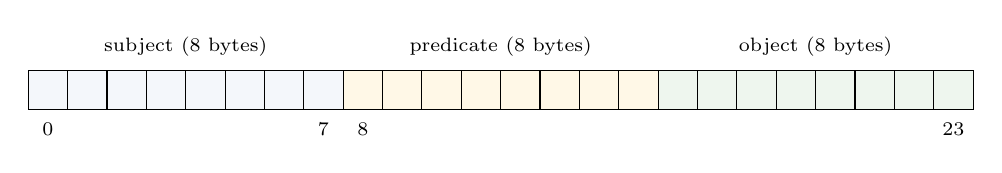
\begin{tikzpicture}[font=\scriptsize]
\foreach \i in {0,...,7}{\node[draw,minimum width=0.5cm,minimum height=0.5cm,fill=boxbg] at (\i*0.5,0) {};}
\foreach \i in {8,...,15}{\node[draw,minimum width=0.5cm,minimum height=0.5cm,fill=ideabg] at (\i*0.5,0) {};}
\foreach \i in {16,...,23}{\node[draw,minimum width=0.5cm,minimum height=0.5cm,fill=statusbg] at (\i*0.5,0) {};}
\node at (1.75,0.55) {subject (8 bytes)};
\node at (5.75,0.55) {predicate (8 bytes)};
\node at (9.75,0.55) {object (8 bytes)};
\node at (0,-0.5) {0}; \node at (3.5,-0.5) {7}; \node at (4,-0.5) {8}; \node at (11.5,-0.5) {23};
\end{tikzpicture}
\caption{A 24-byte triple key: three big-endian unsigned 64-bit ids.}
\label{fig:key}
\end{figure}

Why big-endian: little-endian stores the least significant byte first, so the
id 256 (\code{00 01 00\ldots} in little-endian) would compare below the id 1
(\code{01 00 00\ldots}). With big-endian, integer order and byte order agree,
and the comparison needs no decoding at all.

\section{Prefix scans}

A triple pattern with some positions bound is a \emph{prefix} of the key, if the
bound positions come first. ``Every triple with subject 5'' is every key whose
first 8 bytes encode 5. Such a prefix is a contiguous range of keys, so a scan
is one descent plus a walk along leaves. The range is $[\text{lower},
\text{upper})$, where lower is the prefix padded with zeros and upper is the
prefix's last component plus one:

\begin{center}
\begin{tabular}{@{}cll@{}}
\toprule
Bound components & Lower bound & Upper bound (exclusive) \\
\midrule
0 & \code{(0, 0, 0)} & past every key \\
1 & \code{(5, 0, 0)} & \code{(6, 0, 0)} \\
2 & \code{(5, 7, 0)} & \code{(5, 8, 0)} \\
3 & \code{(5, 7, 9)} & \code{(5, 7, 10)} \\
\bottomrule
\end{tabular}
\end{center}

\section{One ordering is not enough}

An index ordered subject, predicate, object (SPO) serves any pattern whose bound
positions are a prefix of S-P-O. It does not serve ``which subjects have object
\code{Material}?'': the object is the last component, so the matching keys are
scattered across the whole tree. The fix is to store the same triples in more
than one order.

\begin{table}[ht]
\centering
\begin{tabular}{@{}ll@{}}
\toprule
Bound positions in the pattern & Answered as a prefix of \\
\midrule
subject & SPO \\
subject, predicate & SPO \\
predicate & POS \\
predicate, object & POS \\
object & OSP \\
object, subject & OSP \\
all three & any (a point lookup) \\
none & any (a full scan) \\
\bottomrule
\end{tabular}
\caption{Three permutations (SPO, POS, OSP) make every bound/unbound combination a prefix scan.}
\label{tab:perm}
\end{table}

Hexastore \cite{hexastore} keeps all six permutations; RDF-3X \cite{rdf3x} also
keeps six but compresses them heavily and adds aggregated indexes. Each
permutation is another full copy of the triples, so the right number is a
measurement, not a default: three cover every pattern as a prefix, and the
other three only add sorted orders that some joins can exploit.

\begin{keyidea}
Extra permutations change the \emph{cost} of answering a pattern, never the
\emph{answer}. With only SPO, every pattern is still answerable by scanning and
filtering; the other permutations turn scans into prefix ranges.
\end{keyidea}

\begin{ontodb}[: keys, permutations, and the catalog]
OntoDB's \code{TripleKey} is exactly \cref{fig:key}: three big-endian
\code{uint64}s, compared with \code{memcmp}. \code{PrefixLower(key, n)} and
\code{PrefixUpper(key, n)} produce the bounds for $n = 0, 1, 2, 3$ bound
components. The catalog names three B+ tree roots, \code{"spo"}, \code{"pos"},
and \code{"osp"}, and an insert or delete updates every permutation the catalog
has, or none. The plan builds SPO first and then \emph{measures} whether POS and
OSP pay for their space on real SPARQL workloads before adding them.
\end{ontodb}

\begin{status}
The triple key is the next item to implement (plan 0.2). The indexed store and
the permutation measurement follow the B+ tree (plans 3.4 and 3.5).
\end{status}

\section*{Further reading}
Weiss, Karras, and Bernstein \cite{hexastore}; Neumann and Weikum \cite{rdf3x},
the sections on the dictionary and on permutations.

\chapter{The Log-Structured Alternative}
\label{ch:lsm}

A B+ tree updates pages \emph{in place}: an insert finds the right leaf and
changes it. The other great family of storage engines never updates in place.
A \term{log-structured merge tree} (LSM tree), introduced by O'Neil et al.\
\cite{lsm}, turns every write into a sequential append and pays for it later,
in the background. RocksDB, LevelDB, Cassandra, and many modern stores are LSM
trees. Knowing why OntoDB does \emph{not} use one teaches as much as knowing why
it uses a B+ tree.

\section{How an LSM tree works}

\begin{enumerate}
\item \textbf{Memtable.} Writes go to an in-memory sorted structure (often a skip list), and to a write-ahead log for durability.
\item \textbf{Flush.} When the memtable is full, it is written to disk as an immutable sorted file, an \term{SSTable}, in one sequential write.
\item \textbf{Compaction.} SSTables accumulate. A background process merges them into larger SSTables, dropping overwritten and deleted entries. In \term{leveled} compaction, level $L+1$ is about ten times larger than level $L$.
\item \textbf{Reads} check the memtable, then SSTables from newest to oldest, and stop at the first hit.
\item \textbf{Deletes} write a \term{tombstone}, a marker that hides older versions until compaction removes both.
\end{enumerate}

A read that misses must look in many files. \term{Bloom filters}, one per
SSTable, answer ``is this key possibly here?'' in memory with no false
negatives, so most files are skipped without a read.

\section{Three amplifications}

Every storage engine trades three costs against each other.

\begin{description}[leftmargin=1.2em]
\item[Write amplification] Bytes written to the device per byte of user data. An LSM tree rewrites data at every compaction; a B+ tree rewrites a whole page to change a few bytes.
\item[Read amplification] Pages read per lookup. A B+ tree reads one path; an LSM tree may consult several levels.
\item[Space amplification] Bytes stored per byte of live data. LSM trees hold obsolete versions until compaction; B+ trees hold half-empty pages.
\end{description}

\begin{table}[ht]
\centering
\begin{tabular}{@{}lll@{}}
\toprule
& B+ tree & LSM tree \\
\midrule
Writes & random, in place & sequential, batched \\
Point reads & one root-to-leaf path & memtable, then levels (Bloom filters help) \\
Range scans & walk linked leaves & merge iterators across levels \\
Deletes & remove now, merge pages & tombstone now, remove at compaction \\
Background work & none required & compaction, always \\
Best for & read-heavy, range-heavy & write-heavy, ingest-heavy \\
\bottomrule
\end{tabular}
\caption{The two families, in broad strokes.}
\end{table}

\begin{keyidea}
An LSM tree buys fast writes with deferred work. A B+ tree pays for each write
immediately, and gets predictable reads and no background compaction in return.
\end{keyidea}

\begin{ontodb}[: why a B+ tree]
OntoDB's workload is a SPARQL engine's: a bulk load, then queries that are joins
of prefix range scans. Range scans over sorted permutations are a B+ tree's
best case, and bulk loading builds full, sequential leaves without any
compaction. A delete in OntoDB's tree shrinks the tree in place, inside
\code{BPlusTree::Remove}; there is no tombstone for a reader to skip and no
background job that rewrites sorted runs.

The LSM ideas still appear in OntoDB, in smaller roles. Its persistent
databases (\cref{ch:durability}) are log-plus-snapshot: every change is appended
to a log, and a checkpoint rewrites the whole state as one sorted image, which
is a compaction with a single level. And Bloom filters are a natural fit for
``has this concept been modified recently?'' checks over a log.
\end{ontodb}

\begin{checkyourself}
\item A workload inserts 10 million triples per hour and runs few queries. Which family fits better, and what does the other one pay?
\item Why does an LSM delete write a tombstone instead of removing the key?
\item A Bloom filter says ``maybe present'' for a key that is absent. What does that cost an LSM read? Can it say ``absent'' for a present key?
\item In what sense is OntoDB's snapshot-plus-log a one-level LSM tree?
\end{checkyourself}

\section*{Further reading}
O'Neil et al.\ \cite{lsm}; Petrov \cite{petrov}, chapter 7; Bloom
\cite{bloom}.


\part{Query Processing}
\chapter{From SPARQL to a Plan}
\label{ch:plans}

A query states \emph{what} to find. The engine must decide \emph{how}. This
chapter follows a SPARQL query from text to an executable tree of operators,
and introduces the iterator model that runs it.

\section{Parsing and binding}

The \term{parser} turns text into an abstract syntax tree: prefixes, the
projected variables, the triple patterns, the filters. Syntax that the engine
does not support should fail here, with a line and a column, rather than half
work later.

The \term{binder} then resolves names against the database:

\begin{itemize}
\item Prefixed names become full IRIs: \code{ub:Student} becomes\\ \code{<http://example.edu/univ\#Student>}.
\item Every constant becomes a dictionary id. For a query, a constant that is not in the dictionary can match nothing; for an insert, it is added.
\item Every variable gets a \term{slot}: a column number, assigned in order of first appearance.
\end{itemize}

After binding, a row is simply an array of ids indexed by slot. The same
variable in two patterns is the same slot, and that shared slot is the join key.

\section{Logical and physical plans}

A \term{logical plan} says what to compute in terms of algebra: scan each
pattern, join the results, filter, project. A \term{physical plan} picks an
algorithm for each step: which index and range to scan, which join algorithm,
in what order. The planner produces a correct physical plan; the optimizer
(\cref{ch:joins}) rewrites it into a fast one that returns the same rows.

For the query

\begin{lstlisting}
SELECT ?name WHERE {
  ?s a ub:Student . ?s ub:name ?name . ?s ub:age ?age .
  FILTER (?age > 21)
}
\end{lstlisting}

a straightforward plan is left-deep, joining the patterns in the order written:

\begin{lstlisting}
Projection [?name]
  Filter (?age > 21)
    NestedLoopJoin
      NestedLoopJoin
        TripleScan {?s rdf:type ub:Student}
        TripleScan {?s ub:name ?name}
      TripleScan {?s ub:age ?age}
\end{lstlisting}

\section{The iterator (Volcano) model}

Graefe's \term{Volcano} model \cite{graefe} gives every operator the same
three-call interface:

\begin{itemize}
\item \code{Init()}: prepare, or restart from the beginning.
\item \code{Next(\&row)}: produce the next row and return true, or return false when exhausted.
\item destruction: release everything held (for a scan, its pinned leaf).
\end{itemize}

The root operator calls \code{Next} on its child, which calls \code{Next} on
its children, and so on down to the scans. Rows flow up \emph{one at a time},
on demand. Three properties make this model the default for decades:

\begin{description}[leftmargin=1.2em]
\item[Composability.] Any operator can sit above any other, because they share an interface.
\item[Pipelining.] A row can travel from a scan to the client without any intermediate result being materialized. \code{LIMIT 10} stops the whole tree after ten rows.
\item[Bounded memory.] Only operators that must see all their input first (sort, hash-join build, aggregation) hold rows.
\end{description}

Its cost is one virtual call per row per operator. Modern analytical engines
reduce that with \term{vectorized} execution (batches of rows per call) or by
compiling the plan into tight loops, but the logical structure is unchanged.

\begin{keyidea}
Planning builds a tree; execution pulls rows through it. Keeping the two
separate is what allows \code{\textbackslash explain} to print a plan without
running it, and an optimizer to swap one tree for another.
\end{keyidea}

\section{The operators}

\begin{description}[leftmargin=1.2em]
\item[Triple scan.] Reads the triples that match one pattern. With an index, the bound positions choose a permutation and a prefix range (\cref{ch:rdf-indexing}). If a variable occurs twice in one pattern (\code{?x ex:knows ?x}), the scan also checks that those positions are equal.
\item[Join.] Combines rows from two children whose shared slots agree (\cref{ch:joins}).
\item[Filter.] Passes rows whose expression is true. In SPARQL a type error makes the expression false, not the query fail.
\item[Projection.] Keeps the selected slots.
\item[Distinct, limit, offset, sort.] Distinct applies to \emph{projected} rows (two triples can share a name). Sort compares values, not ids: ids are assigned in load order, which is not value order.
\end{description}

\begin{ontodb}[: planning and execution]
OntoDB's binder assigns slots in first-appearance order and represents ``not yet
bound'' with a reserved id. The planner always produces the left-deep tree in
textual order with nested-loop joins, which is correct but rarely fast;
\code{\textbackslash explain} prints it. An executor factory maps each plan node
to its executor, and the engine pulls rows with \code{Init}/\code{Next}.
An empty pattern, with no triple to match, returns one empty row rather than
none: the identity input for a join that has nothing to bind yet.
\end{ontodb}

\begin{decision}{Unsupported syntax fails at parse time}
\dpart{Choice} \code{OPTIONAL}, \code{UNION}, property paths, aggregates, and
\code{DELETE/INSERT WHERE} are recognized by the parser and rejected there with
a line and column.
\dpart{Alternatives} Accept the full grammar and fail in the executor; or skip
what is not understood.
\dpart{Why} A query either runs completely or fails before anything happens.
Ignoring an \code{OPTIONAL} would silently change the answer, which is worse
than refusing.
\dpart{Cost} The parser must know the shape of features the engine does not
implement.
\end{decision}

\begin{decision}{Volcano, one row at a time}
\dpart{Choice} Every operator implements \code{Init} and \code{Next} and passes
one row of ids per call.
\dpart{Alternatives} Vectorized execution (a batch of rows per call), or
compiling the plan into loops.
\dpart{Why} It is the simplest model that composes, it makes \code{LIMIT} stop
the whole tree, and it keeps pin ownership obvious: a scan holds one leaf while
it has a current row.
\dpart{Cost} A virtual call per row per operator. Large analytical scans would
be several times faster vectorized.
\end{decision}

\begin{decision}{Stub plan nodes before their executors}
\dpart{Choice} \code{Sort}, \code{Distinct}, \code{Limit}, \code{Insert}, and
\code{Delete} exist as plan nodes that \code{\textbackslash explain} prints
before their executors are written.
\dpart{Alternatives} Add a plan node only together with its executor.
\dpart{Why} The plan's shape and the planner's tests can be fixed first; each
executor then arrives into a slot that is already wired and printed.
\dpart{Cost} For a while, \code{\textbackslash explain} shows plans that cannot
run, and running one throws ``not built yet''.
\end{decision}

\begin{decision}{\code{DISTINCT} keeps a hash set}
\dpart{Choice} The distinct operator passes a row the first time it sees it,
in its child's order, and remembers every row it has passed in a hash set.
\dpart{Alternatives} Sort the rows and drop adjacent duplicates.
\dpart{Why} Hashing streams: the first answer comes out as soon as it is
found, \code{LIMIT} above it still stops early, and the order the child chose
is kept.
\dpart{Cost} Memory grows with the number of distinct rows. A sort-based
distinct could spill to disk; this one cannot.
\end{decision}

\begin{decision}{Rows have no order without \code{ORDER BY}}
\dpart{Choice} The engine promises no order unless the query has
\code{ORDER BY}. Tests compare answers as multisets.
\dpart{Alternatives} Always return rows in a fixed order, for example sorted by
id.
\dpart{Why} The order a plan produces depends on the store, the indexes, and
the join operator: the memory store returns triples in insertion order, the
indexed store in key order. Promising an order would force a sort on every
query.
\dpart{Cost} \code{LIMIT} without \code{ORDER BY} may return different rows on
the two backends, or under different join operators. Both answers are correct,
which is why the differential test checks such queries only when the limit is
larger than the answer.
\end{decision}

\begin{status}
Parsing, binding, planning, triple scans, the three joins, filter,
projection, distinct, limit, and offset run on both backends (plans 4.1 to
4.4). Sort is parsed and planned; its executor is plan 4.5.
\end{status}

\begin{checkyourself}
\item In \code{?s a ub:Student . ?s ub:name ?name . ?s ub:age ?age}, which slot does each variable get?
\item Why does \code{DISTINCT} apply to projected rows, not to the rows the scans produce?
\item Why can't \code{ORDER BY} compare term ids?
\item A plan is \code{Limit 10} over a join of two large scans. How much work does the Volcano model do, and how much would a model that materializes each operator's output do?
\item Why does an empty pattern produce one empty row rather than none?
\item \code{SELECT ?name WHERE \{ ... \} LIMIT 2} returns Alice and Bob on the memory backend and Alice and Cara on the indexed one. Which is wrong?
\end{checkyourself}

\section*{Further reading}
Graefe \cite{graefe}; the W3C SPARQL 1.1 recommendation \cite{sparql}.

\chapter{Joins and Query Optimization}
\label{ch:joins}

A SPARQL query of $k$ triple patterns is a $k$-way join, and its running time
depends far more on \emph{how} it is joined than on anything else. This chapter
covers the three join algorithms, how an optimizer estimates the size of
intermediate results, and how it searches for a good join order.

\section{Three join algorithms}

Let the outer input have $|R|$ rows and the inner input $|S|$ rows.

\paragraph{Nested-loop join.} For each outer row, scan the whole inner input and
keep the pairs whose shared slots agree. Cost: $|R| \times |S|$ comparisons, no
extra memory. Correct for any join, and the fallback when nothing better applies.

\paragraph{Index nested-loop join.} For each outer row, substitute its bindings
into the inner pattern and \emph{probe an index} for just the matching triples.
If the outer row binds the subject and SPO exists, the inner side becomes a
prefix range, often one or a handful of triples. Cost: $|R|$ index probes. This
is the common, fast case in SPARQL: one pattern finds the entities, and each
further pattern looks up an attribute of each entity.

\paragraph{Hash join.} \emph{Build} a hash table on the shared slots of one input
(ideally the smaller), then \emph{probe} it with each row of the other. Cost:
linear in $|R| + |S|$, plus memory for the build side. It wins when both inputs
are large and no index makes the probe selective, and it loses when the build
side does not fit in memory, or when an index probe was already a point lookup.

\begin{keyidea}
Index nested loop is fast when the outer side is small and the inner side is
indexed on the join key; hash join is fast when both sides are large; nested
loop is always correct. An optimizer's job is to know which case it is in.
\end{keyidea}

\section{Cardinality estimation}

To compare plans, the optimizer needs the \term{cardinality} of each
intermediate result: how many rows each operator produces. It estimates them
from \term{statistics} gathered at load time: the total triple count $|T|$,
the number of distinct subjects, predicates, and objects, and per-predicate
counts.

For a pattern with predicate $p$ and object $o$ bound, the classic estimate
assumes the positions are \term{independent}:
\[
  \widehat{\,|\{(s,p,o)\}|\,} \;=\; \frac{|p| \cdot |o|}{|T|},
\]
where $|p|$ and $|o|$ are the counts of triples with that predicate and that
object. Independence is convenient and frequently wrong. In RDF, predicates and
objects are strongly correlated (\code{rdf:type} goes with class objects; a
\code{name} predicate never has a class as its object), so independence can be
off by orders of magnitude.

The \term{q-error} measures an estimate $\hat c$ against the true count $c$:
\[
  q(\hat c, c) = \max\!\left(\frac{\hat c}{c},\ \frac{c}{\hat c}\right) \ \ge 1 .
\]
It treats over- and underestimates symmetrically, and errors multiply as they
propagate up a plan: a join of two inputs each off by 10 can be off by 100.

\section{Searching for a join order}

A left-deep plan over $k$ patterns has $k!$ orders, and each join can use
several algorithms. Selinger's System R optimizer \cite{selinger} made the
search tractable with dynamic programming:

\begin{lstlisting}[language=pseudo]
for each single pattern P:   best[{P}] = cheapest access path for P
for size = 2 to k:
  for each subset S of patterns with |S| = size:
    for each pattern P in S:
      candidate = join(best[S - {P}], P) with the cheapest algorithm
      if cost(candidate) < cost(best[S]): best[S] = candidate
return best[all patterns]
\end{lstlisting}

It keeps one best plan per subset rather than per order, which reduces $k!$ to
about $k \cdot 2^k$. A simpler \term{greedy} strategy (start with the most
selective pattern, then repeatedly add the cheapest connected pattern) is a
good first step and often good enough for the star-shaped joins common in SPARQL.

\section{Explain analyze}

The single most useful optimizer tool is to \emph{run} the plan and print, next
to each operator's estimated rows, the rows it actually produced. The node where
the two diverge most is where a statistic is missing, usually a correlation that
the independence assumption averaged away.

\begin{ontodb}[: the optimizer]
OntoDB's optimizer takes the planner's tree and returns another tree that must
return the same rows. The shell setting \code{\textbackslash set join
auto|nlj|inlj|hash} either lets it choose or forces one algorithm, and forcing
happens in the optimizer, not the executor, so the plan that
\code{\textbackslash explain} prints is always the plan that runs. Statistics
are collected at load: the triple count, distinct counts per position,
per-predicate counts, and counts for partially bound patterns. Estimates are
finite, never negative, and binding one more position never increases them.
Join ordering starts greedy and left-deep.
\end{ontodb}

\begin{decision}{Exact counts for single patterns}
\dpart{Choice} Statistics are collected in one scan of the store: counts per
subject, predicate, and object, per pair of positions, and the set of triples.
Every single triple pattern of constants therefore has an \emph{exact}
cardinality; estimation, and its independence assumptions, begin only at joins.
\dpart{Alternatives} Distinct counts and per-predicate counts only, combined
with the independence formula above; histograms or samples; or RDF-3X's
characteristic sets, which summarize which predicates occur together on one
subject.
\dpart{Why} The independence formula is wrong by orders of magnitude on RDF,
where predicates and objects are correlated. For a store of this size, exact
pair counts are affordable and remove that error from every scan estimate.
\dpart{Cost} About seven hash entries per triple, collected at load, and
stale after updates until the next collection, like a table that has not been
re-\code{ANALYZE}d.
\end{decision}

\begin{decision}{Join estimates use distinct values}
\dpart{Choice} A join's estimate is System R's
$|L|\,|R| / \max(V(L,x), V(R,x))$ for each shared variable $x$, where $V$ is
the number of distinct values $x$ takes. For a single pattern, $V$ comes from
statistics: a predicate's distinct subjects or objects, or the pattern's own
count when the other positions are bound.
\dpart{Alternatives} Assume each side's join values are all distinct, which
gives $\min(|L|, |R|)$ for one shared variable; or a fixed selectivity per join.
\dpart{Why} SPARQL joins come in two shapes that the simple rule cannot both
get right. On a store of 100 students taking 3 of 10 courses, joining students
to their names (a star on the subject) is 100 rows, and joining enrolments to
the course class is 300. Distinct values give both exactly; $\min(|L|,|R|)$
says 10 for the second, 30 times too low.
\dpart{Cost} Two more counts per predicate, and an assumption that remains: the
join values of the smaller side are taken to appear on the larger side. A
variable's $V$ in an intermediate result is approximated by the smaller of its
$V$ in a pattern and the result's size.
\end{decision}

\begin{decision}{The inner side is re-opened with the outer row}
\dpart{Choice} Every executor has \code{InitWith(row)}, which by default is
\code{Init}. A triple scan overrides it: each variable that the outer row
already binds becomes a constant in the pattern it hands the store. The nested
loop re-opens its inner side this way for every outer row.
\dpart{Alternatives} Open the inner scan once with its own pattern and compare
every inner row with every outer row; or materialize the inner side once and
loop over the copy.
\dpart{Why} With the outer row filled in, the inner pattern usually binds the
subject, so on an indexed store each probe is a short prefix range instead of
a scan of every triple with that predicate. The cost per outer row drops from
the size of the inner pattern to the size of its match.
\dpart{Cost} One store scan opened, and one tree descent, per outer row, with
no caching between rows that bind the same values.
\end{decision}

\begin{decision}{Index nested loop probes the store directly}
\dpart{Choice} The index nested-loop join requires its inner side to be one
triple pattern. It has no inner executor: for each outer row it builds the
probe pattern from the outer row and asks the store, which picks the index
whose order starts with the bound positions.
\dpart{Alternatives} Treat any nested loop over a rebound scan as an index
nested loop, since with rebinding it already probes.
\dpart{Why} With rebinding, the nested loop already probes an index, so the
two operators read the same triples. The separate operator skips the inner
executor and the generic row merge, and it names the strategy in the plan,
where \code{\textbackslash explain} and the optimizer can see it.
\dpart{Cost} Only a scan can be the inner side; a join whose inner side is
itself a join stays a nested loop.
\end{decision}

\begin{decision}{Hash join builds on the inner side}
\dpart{Choice} The hash join reads its inner (right) input once into a table
keyed by the ids of the variables both sides produce, then streams the outer
input through it. A row whose key slot is unbound is not hashed but compared
with every row of the other side.
\dpart{Alternatives} Build on whichever side is smaller, or partition both
sides to disk when the table does not fit (a grace hash join).
\dpart{Why} Choosing the smaller side needs cardinality estimates, which
arrive with the optimizer (plans 5.1 and 5.2); until then the inner side of a
left-deep plan is a single pattern, usually the smaller input.
\dpart{Cost} The whole inner side lives in memory; a large inner pattern can
make the build expensive or exhaust memory. There is no spilling.
\end{decision}

\begin{decision}{Forcing a join method rewrites the plan}
\dpart{Choice} \code{\textbackslash set join hash} (or \code{nlj}, \code{inlj})
is applied by the optimizer (\code{Optimizer::ApplyJoinMethod}), which swaps
each nested-loop node for the chosen one before the plan is explained or run.
The executor factory only reads node types.
\dpart{Alternatives} Keep one join node and let the executor read the setting
at run time.
\dpart{Why} \code{\textbackslash explain} then always prints the plan that
runs. A test can check that a forced hash plan contains a hash join without
running it.
\dpart{Cost} The optimizer must be invoked even when the user forces
everything.
\end{decision}

\begin{decision}{Greedy, left-deep join ordering first (planned)}
\dpart{Choice} Start from the most selective pattern and repeatedly add the
cheapest pattern connected to what is already joined, producing a left-deep
tree.
\dpart{Alternatives} Selinger's dynamic programming over subsets, or a search
that also considers bushy trees.
\dpart{Why} Most SPARQL basic graph patterns are stars around one subject, for
which greedy is close to optimal, and a greedy order is easy to explain in
\code{\textbackslash explain analyze}.
\dpart{Cost} Chains and snowflakes, where a bushy plan or a non-greedy first
step wins, can be ordered badly.
\end{decision}

\begin{status}
Today the planner always joins in textual order with nested loop, and the
nested loop rebinds its inner scan for every outer row (plan 4.1). The index
nested-loop join (plan 4.2) and hash join (plan 4.3) run, chosen with
\code{\textbackslash set join}, and the differential test checks every query
file under all three against the memory store. Statistics (plan 5.1) and cardinality estimation (plan 5.2) run. Join
ordering, the automatic choice, and \code{\textbackslash explain analyze} are
plans 5.3 to 5.5.
\end{status}

\begin{checkyourself}
\item Outer side 1,000 rows, inner pattern 1,000,000 triples, and the join binds the inner subject with SPO available. Compare nested loop and index nested loop.
\item When does a hash join beat index nested loop?
\item With exact pair counts, what is OntoDB's estimate for \code{(?, p, o)}, and where can its estimates still go wrong?
\item A store has $|T| = 10^6$, $|p| = 10^4$, $|o| = 10^3$. What does the independence formula estimate for \code{(?, p, o)}? The true count is 1,000. What is the q-error?
\item Why do estimation errors multiply up a plan?
\item A hash join builds on \code{?c a ub:Course} (2,000 rows) and probes with \code{?s ub:takesCourse ?c} (50,000 rows). What does it keep in memory, and how many hash lookups does it make? What changes if the sides are swapped?
\item \code{?s a ub:Student . ?s ub:name ?n}: the first pattern matches 1,000 students and the second 1,000,000 triples. How many triples does the nested loop read with rebinding on an indexed store, and how many without it?
\item Why does forcing a join method in the optimizer, and not in the executor, matter for \code{\textbackslash explain}?
\end{checkyourself}

\section*{Further reading}
Selinger et al.\ \cite{selinger}; Graefe \cite{graefe}; Leis et al.\
\cite{leis2015} on how good cardinality estimates really are; Neumann and
Weikum \cite{rdf3x} on RDF selectivity.

\chapter{Beyond Basic Graph Patterns}
\label{ch:sparql}

A basic graph pattern is a conjunction: every triple pattern must match, or the
row is gone. Most questions people ask of an ontology are not conjunctions.
``List every material, with its melting point \emph{if we know it}'' keeps a
material whose melting point is missing. ``Metals or ceramics'' is a
disjunction. ``How many subclasses does each class have'' collapses rows into
groups. This chapter adds the operators behind those questions, \code{OPTIONAL},
\code{UNION}, and aggregation, and the update form whose triples come from a
query. Each one is a relational operator the earlier chapters did not need,
and each one constrains the optimizer in a way an inner join does not.

\section{Where a conjunction loses rows}

Take three materials, two of them with a melting point:
\begin{lstlisting}
:Steel   :meltsAt 1370 .
:Copper  :meltsAt 1085 .
:Steel a :Material .  :Copper a :Material .  :Glass a :Material .
\end{lstlisting}
The pattern \code{\{ ?m a :Material . ?m :meltsAt ?t \}} is a join of two
scans on \code{?m} (\cref{ch:joins}), and it returns two rows. \code{Glass} is
not wrong; it is unknown, and the inner join cannot say ``unknown''. The fix is
an operator whose output keeps every row of one side.

\section{OPTIONAL is a left outer join}

SPARQL's algebra works on \term{solution mappings}: partial functions from
variables to terms. Two mappings are \term{compatible} when they agree on every
variable both bind. For multisets of mappings $\Omega_1$ and $\Omega_2$ and a
filter expression $e$ \cite{sparql,perez2009}:
\[
\mathit{LeftJoin}(\Omega_1, \Omega_2, e) \;=\;
\mathit{Filter}\big(e, \mathit{Join}(\Omega_1, \Omega_2)\big) \;\cup\;
\{\, \mu_1 \in \Omega_1 \mid \neg\exists \mu_2 \in \Omega_2 :\ \mu_1 \sim \mu_2 \wedge e(\mu_1 \cup \mu_2) \,\}.
\]
The first part is the inner join; the second keeps each left mapping that found
no compatible partner, with the right side's variables \term{unbound}. For the
example, \code{?m a :Material OPTIONAL \{ ?m :meltsAt ?t \}} gives:

\begin{center}
\begin{tabular}{@{}ll@{}}
\toprule
\code{?m} & \code{?t} \\
\midrule
\code{:Steel} & 1370 \\
\code{:Copper} & 1085 \\
\code{:Glass} & \emph{(unbound)} \\
\bottomrule
\end{tabular}
\end{center}

An unbound value is not a value. It is a hole in the row, and the executor has
to carry it: rows gain a ``not bound'' marker per column, which the result
printer shows as an empty cell.

\subsection{A filter inside OPTIONAL is part of the join}

The $e$ in the definition matters. Compare
\begin{lstlisting}
SELECT ?m ?t WHERE { ?m a :Material OPTIONAL { ?m :meltsAt ?t FILTER(?t > 1200) } }
SELECT ?m ?t WHERE { ?m a :Material OPTIONAL { ?m :meltsAt ?t } FILTER(?t > 1200) }
\end{lstlisting}
The first keeps all three materials: \code{Steel} with 1370, and \code{Copper}
and \code{Glass} with \code{?t} unbound, because the filter only decides which
right rows may join. The second filters the finished rows, and a comparison
with an unbound value is an \emph{error}, which \code{FILTER} treats as false: it
returns \code{Steel} alone. Moving a filter across an \code{OPTIONAL} boundary
changes the answer, so the planner must not do it.

\begin{keyidea}
An outer join is not commutative, and filters do not move freely across it. The
left side is preserved; the right side only decorates it.
\end{keyidea}

\section{Executing a left join}

Both join algorithms of \cref{ch:joins} extend to outer joins with one extra bit
of state.

\begin{description}[leftmargin=1.2em]
\item[Nested loop.] For each left row, rebind and scan the right side. If no
right row matched (after the join filter), emit the left row once with the
right columns unbound. The bit is ``did this left row match'', and it lives for
one iteration of the outer loop.
\item[Hash join.] Build the hash table on the \emph{right} side and probe with
the left. A probe that finds no partner emits the left row padded. If the build
side were the left one, every left row would need a ``matched'' flag in the
table and a final pass over the table to emit the unmatched ones; that works,
but it makes the operator blocking at its end as well as its start.
\end{description}

An index nested-loop left join is the common case in practice: the left side
is a selective pattern, and the optional part is a lookup by subject on SPO.

\begin{decision}{Left joins build on the right (planned)}
\dpart{Choice} The hash left join builds on the optional (right) side and
probes with the preserved (left) side.
\dpart{Alternatives} Build on the left with a matched flag per entry, and emit
unmatched entries after the probe phase.
\dpart{Why} Padding happens at probe time, the operator streams its output,
and the optimizer's choice is only whether the right side fits in memory.
\dpart{Cost} When the right side is much larger than the left, building on it
costs memory a left build would not.
\end{decision}

\section{UNION}

\code{\{ P1 \} UNION \{ P2 \}} evaluates both sides and concatenates their rows.
SPARQL union is a bag union: a row produced by both sides appears twice, and
\code{DISTINCT} removes duplicates across sides. The sides may bind different
variables, so a row from one side has the other side's variables unbound, the
same marker \code{OPTIONAL} introduced. The executor is the simplest operator in
the engine, a concatenation of two child iterators; the work is in the binder,
which computes the output columns as the union of both sides' variables.

\section{Aggregation}

\code{GROUP BY} partitions rows by the values of its keys and computes one row
per group:
\begin{lstlisting}
SELECT ?c (COUNT(?sub) AS ?n) WHERE { ?sub rdfs:subClassOf ?c }
GROUP BY ?c HAVING (COUNT(?sub) > 2)
\end{lstlisting}
There are two classic implementations \cite{graefe}:
\begin{description}[leftmargin=1.2em]
\item[Sort aggregation.] Sort by the group keys (the external merge sort of
\cref{ch:joins} already exists), then scan once, finishing a group whenever the
key changes. Output comes out ordered by the keys.
\item[Hash aggregation.] Keep a hash table from group key to an accumulator and
update it per row. One pass, no sort, but the table must hold every group.
\end{description}
Accumulators are small: \code{COUNT} is a counter, \code{SUM}, \code{MIN}, and
\code{MAX} one value, \code{AVG} a sum and a count, divided at the end.
\code{COUNT(DISTINCT x)} is the exception: it needs the set of distinct values
per group, so its memory grows with the data, not with the number of groups.
\code{HAVING} is a filter on the output of the aggregation.

\begin{decision}{Hash aggregation, and what to do when groups outgrow memory (planned)}
\dpart{Choice} Hash aggregation. When the table exceeds its memory budget,
the plan records whether to spill or refuse; the leading design is to partition
the input by a hash of the key into files, then aggregate each partition in
memory, as hybrid hash join does for joins.
\dpart{Alternatives} Sort aggregation always; or refuse with a clear error past
the budget.
\dpart{Why} Ontology workloads group by class or property, and there are far
fewer of those than triples, so the table almost always fits and one pass
beats a sort.
\dpart{Cost} Output is unordered, so \code{ORDER BY} on the keys still sorts;
the spill path is code that runs rarely, which is why it needs its own tests.
\end{decision}

\section{Planning around the new operators}

The join-order search of \cref{ch:joins} treats a basic graph pattern as a set
of patterns to permute. With \code{OPTIONAL}, the pattern becomes a tree, and
only parts of it may be reordered:
\begin{itemize}
\item Patterns inside the left side may be reordered among themselves, and so
may patterns inside the right side. A pattern may not move from one side of an
\code{OPTIONAL} to the other: that would turn an optional match into a required
one, or the reverse.
\item The cardinality of a left join is at least that of its left side, since
every left row survives. An estimate below that is a bug, not a guess.
\item \code{\textbackslash explain analyze} shows the new operators with
estimated and actual rows, as it does for joins, so a bad estimate is visible.
\end{itemize}
Pérez, Arenas, and Gutierrez \cite{perez2009} identify the \term{well-designed}
patterns, those where every variable shared between an optional part and the
outside also appears on the left; for them, more rewrites are safe, and
evaluation is easier. Patterns written by people are almost always
well-designed.

\section{Updates whose triples come from a query}

\code{DELETE \{ \ldots \} INSERT \{ \ldots \} WHERE \{ \ldots \}} rewrites every
match: move every class under \code{:Metal} to \code{:MetallicMaterial},
for example. The order of the three parts is the whole semantics:

\begin{enumerate}
\item Evaluate the \code{WHERE} pattern \emph{in full}, producing every solution.
\item Instantiate and delete the \code{DELETE} templates for every solution.
\item Instantiate and insert the \code{INSERT} templates for every solution.
\end{enumerate}

Interleaving them is wrong for the same reason as the \emph{Halloween problem}
of relational updates: a scan that sees its own inserts can match them again,
and an update that adds a superclass link per subclass could loop forever or
apply twice. Materializing the solutions first gives the update a snapshot of
the data as it was before the statement, which is what the specification
means. The whole statement is one transaction, under the same two-phase locks
as \code{INSERT DATA} and \code{DELETE DATA} (\cref{ch:concurrency}).

\begin{decision}{Evaluate WHERE first, then delete, then insert (planned)}
\dpart{Choice} The solutions of \code{WHERE} are materialized before any triple
changes; deletes run before inserts.
\dpart{Alternatives} Pipeline solutions straight into the updates; or insert
before delete.
\dpart{Why} It is the specification's semantics and it avoids the Halloween
problem. Deleting first means a triple both deleted and inserted by one
statement ends up present, which is what a rewrite intends.
\dpart{Cost} The solutions are held in memory (or spilled) for the statement's
duration.
\end{decision}

\begin{status}
Planned (plan 12.1--12.5): today \code{OPTIONAL}, \code{UNION}, aggregates, and
\code{DELETE/INSERT WHERE} are parsed far enough to fail with a line and a
column. Every new form will run on both backends and join the differential test
that compares the indexed store with the memory store.
\end{status}

\begin{checkyourself}
\item Write the rows of \code{?m a :Material OPTIONAL \{ ?m :meltsAt ?t FILTER(?t < 1200) \}} for the three materials above.
\item Why can a hash left join not simply swap its build and probe sides when the left side is smaller, as an inner hash join can?
\item A union's left side binds \code{?a} and its right side binds \code{?b}. What columns does the result have, and what is in them?
\item Why does \code{COUNT(DISTINCT ?x)} need more memory than \code{COUNT(?x)}, and how does that interact with hash aggregation?
\item An optimizer estimates 40 rows for a left join whose left input it estimates at 100. What is wrong?
\item \code{INSERT \{ ?c rdfs:subClassOf :Thing \} WHERE \{ ?c rdfs:subClassOf ?d \}} runs with the inserts visible to the scan. What can go wrong, and how does materializing \code{WHERE} first prevent it?
\end{checkyourself}

\section*{Further reading}
The SPARQL 1.1 specification \cite{sparql}, section 18, defines the algebra;
Pérez, Arenas, and Gutierrez \cite{perez2009} give its semantics and
complexity, including well-designed patterns; Graefe's survey \cite{graefe}
covers outer joins and hash and sort aggregation.

\chapter{Materialized Inference}
\label{ch:inference}

An ontology says more than it stores. If \code{Alloy subClassOf Metal} and
\code{Metal subClassOf Material}, then every alloy is a material, though no
triple says so; \cref{ch:engine} ended on exactly that gap, with a query for
materials that missed \code{Alloy}. A store that answers ontology queries has
to close it. This chapter treats inference as a database problem: the
entailed triples are a \emph{view} of the stored ones, and the questions are
the old ones for views: compute it on read, or store it and keep it current on
every write.

\section{Two ways to answer with entailments}

\begin{description}[leftmargin=1.2em]
\item[Rewrite at read time] (backward chaining). Turn \code{?x a :Material}
into \code{?x a ?c . ?c rdfs:subClassOf* :Material}, a property path, and let
the executor follow it. Nothing extra is stored; every query pays for the
closure it needs, and a query planner must estimate a recursive path.
\item[Materialize at write time] (forward chaining). Compute every entailed
triple once, store it in the same indexes, and answer \code{?x a :Material}
with one scan of POS, as if the triples had been asserted. Reads stay as fast
as they are; writes and space pay.
\end{description}

\begin{center}
\begin{tabular}{@{}lll@{}}
\toprule
& Rewrite & Materialize \\
\midrule
Read cost & a recursive path per query & one scan \\
Write cost & none & maintain the closure \\
Space & asserted triples & asserted plus entailed \\
Planner & estimate recursion & unchanged \\
\bottomrule
\end{tabular}
\end{center}

Ontologies are read far more often than they change, and their queries ask
for classes \emph{and} their subclasses almost every time, so OntoDB
materializes, like RDFox and GraphDB.

\section{The rules}

RDFS entailment is a handful of rules \cite{rdfsemantics}. Written as Datalog,
with \code{T(s,p,o)} for ``the store holds triple $(s,p,o)$'':
\begin{align*}
T(c, \mathit{sc}, e) &\leftarrow T(c, \mathit{sc}, d),\ T(d, \mathit{sc}, e) && \text{(rdfs11, subclass is transitive)}\\
T(x, \mathit{type}, d) &\leftarrow T(x, \mathit{type}, c),\ T(c, \mathit{sc}, d) && \text{(rdfs9, types go up)}\\
T(p, \mathit{sp}, r) &\leftarrow T(p, \mathit{sp}, q),\ T(q, \mathit{sp}, r) && \text{(rdfs5, subproperty is transitive)}\\
T(x, q, y) &\leftarrow T(x, p, y),\ T(p, \mathit{sp}, q) && \text{(rdfs7, triples go up)}\\
T(x, \mathit{type}, c) &\leftarrow T(x, p, y),\ T(p, \mathit{domain}, c) && \text{(rdfs2)}\\
T(y, \mathit{type}, c) &\leftarrow T(x, p, y),\ T(p, \mathit{range}, c) && \text{(rdfs3)}
\end{align*}
Each rule body is a two-pattern basic graph pattern, so each rule is one join
of two scans, and the executor of \cref{ch:joins} already evaluates it. The
closure is the least set of triples containing the data and closed under the
rules.

\section{Naive and semi-naive evaluation}

The obvious way to compute the closure is to apply every rule to everything,
add what is new, and repeat until a round adds nothing. That is
\term{naive evaluation}, and it is wasteful: round $i$ rederives every triple of
rounds $1$ to $i-1$ before finding the new ones.

The fix is to notice that a triple can be new in round $i$ only if one of the
triples it was derived from was new in round $i-1$. \term{Semi-naive
evaluation} \cite{alicebook} keeps the set $\Delta$ of triples new in the last
round and evaluates each rule with at least one body pattern restricted to
$\Delta$:
\[
\Delta_{i+1} \;=\; \Big(\textstyle\bigcup_{\text{rules}}\ \big(\Delta_i \Join T_i\big) \cup \big(T_i \Join \Delta_i\big)\Big) \setminus T_i,
\qquad T_{i+1} = T_i \cup \Delta_{i+1}.
\]
For a chain of subclasses $A \sqsubseteq B \sqsubseteq C \sqsubseteq D \sqsubseteq E$:

\begin{center}
\begin{tabular}{@{}lll@{}}
\toprule
Round & $\Delta$ (new subclass triples) & Joins evaluated \\
\midrule
0 & the 4 asserted links & --- \\
1 & $A{\sqsubseteq}C$, $B{\sqsubseteq}D$, $C{\sqsubseteq}E$ & $\Delta_0 \times T_0$ \\
2 & $A{\sqsubseteq}D$, $A{\sqsubseteq}E$, $B{\sqsubseteq}E$ & $\Delta_1 \times T_1$ \\
3 & (none) & $\Delta_2 \times T_2$; stop \\
\bottomrule
\end{tabular}
\end{center}

Naive evaluation would rejoin all four asserted links in every round. On a
deep hierarchy the difference is the difference between joining the frontier
and joining the whole closure, round after round.

\begin{keyidea}
Inference is recursive query evaluation, and semi-naive evaluation is to
recursion what a delta is to an update: only what changed can cause anything
new.
\end{keyidea}

\section{Keeping the closure current}

\subsection{Insert}

An inserted triple is a closure computation that starts small: run the same
rounds with $\Delta_0 = \{t\}$, inside the inserting transaction, so that the
closure is complete when the transaction commits. Inserting
\code{Bronze subClassOf Alloy} into a hierarchy above it derives \code{Bronze
subClassOf Metal} and \code{Bronze subClassOf Material} in two rounds, and the
types of every bronze instance in the same rounds.

\subsection{Delete is harder}

Deleting \code{Alloy subClassOf Metal} should remove \code{Alloy subClassOf
Material}, unless it still follows some other way, for example because a
curator also asserted \code{Alloy subClassOf Material} directly. A triple can
have several derivations, and deleting one support must not delete a triple
another support still holds. Two classic answers \cite{gupta1993}:

\begin{description}[leftmargin=1.2em]
\item[Counting.] Store, for each triple, how many derivations it has; a delete
decrements the counts of what it supported and removes triples whose count
reaches zero. Exact for non-recursive rules, but under recursion a triple can
support itself through a cycle, and its count never reaches zero.
\item[Delete and rederive (DRed).] Three steps: (1) \emph{overdelete}:
remove the deleted triple and, by semi-naive rounds, everything it could have
helped derive; (2) \emph{rederive}: for each overdeleted triple, check whether
it still follows in one step from what remains, and put it back if so; (3)
propagate the rederived triples by semi-naive insertion.
\end{description}

\begin{figure}[ht]
\centering
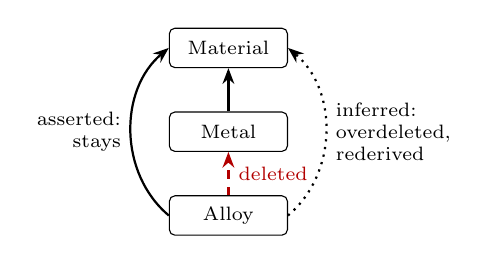
\begin{tikzpicture}[font=\scriptsize,node distance=0.55cm and 1.2cm,
  cls/.style={draw,rounded corners=2pt,minimum width=1.5cm,minimum height=0.5cm,fill=white}]
\node[cls] (al) {Alloy};
\node[cls,above=of al] (me) {Metal};
\node[cls,above=of me] (ma) {Material};
\draw[arrow,dashed,red!70!black] (al) -- node[right]{deleted} (me);
\draw[arrow] (me) -- (ma);
\draw[arrow] (al.west) to[bend left=50] node[left,align=right]{asserted:\\stays} (ma.west);
\draw[arrow,dotted] (al.east) to[bend right=50] node[right,align=left]{inferred:\\overdeleted,\\rederived} (ma.east);
\end{tikzpicture}
\caption{DRed on one delete. Overdeletion removes the inferred \code{Alloy
subClassOf Material}; rederivation finds it is also asserted, so the triple
is back before the transaction commits.}
\end{figure}

DRed is correct with recursion because rederivation asks a positive question,
``does this follow from what remains'', instead of trusting a count. Its cost is
that one delete near the top of a hierarchy overdeletes a large part of the
closure and rederives most of it.

\begin{decision}{Materialize, and maintain with DRed (planned)}
\dpart{Choice} Entailed triples are computed by semi-naive evaluation, stored
in the indexes, extended on insert, and maintained on delete by delete and
rederive. \code{\textbackslash set inference rdfs|off}, off by default.
\dpart{Alternatives} Query rewriting with property paths; counting
derivations; recomputing the closure from scratch after each delete.
\dpart{Why} Reads stay one scan and the planner stays unchanged. DRed is
correct under recursion, which counting is not, and it touches only what the
deleted triple could have supported.
\dpart{Cost} More triples and more index work per write, and a delete high in
a hierarchy is expensive. A test checks after random inserts and deletes that
the store equals a closure computed from scratch.
\end{decision}

\begin{decision}{Where inferred triples live (planned)}
\dpart{Choice} To be decided by measurement: a mark on each triple in the
existing SPO, POS, and OSP indexes, or separate permutations for inferred
triples that scans also read.
\dpart{Alternatives} The two above.
\dpart{Why} A mark keeps one scan per pattern but makes deleting all inferred
triples (\code{\textbackslash set inference off}) a full pass; separate
permutations make that a drop, but double the scans of every pattern.
\dpart{Cost} Either way, a delete must know which triples were asserted, so an
asserted triple that is also inferred keeps its asserted status.
\end{decision}

\section{What it costs}

Materialization trades space and write time for read time, and the exchange
rate depends on the hierarchy's depth. A triple deep in a hierarchy of depth
$d$ entails up to $d$ type triples, and a subclass chain of $n$ classes has
$n(n-1)/2$ entailed links. LUBM's ontology is shallow, so its closure adds a
modest fraction of triples; an anatomy ontology several levels deep adds many
more. The plan measures load time and size with and without inference on
LUBM(1), and checks that the LUBM queries that need RDFS return the official
answer counts.

\begin{status}
Planned (plan 13.1--13.5). Today OntoDB stores OWL as triples and has no
reasoner: the query for materials in \cref{ch:engine} misses \code{Alloy}, as
it should.
\end{status}

\begin{checkyourself}
\item Give one workload for which rewriting at read time beats materializing, and one for which it does not.
\item Run semi-naive evaluation on $A \sqsubseteq B$, $B \sqsubseteq C$ and the type triple \code{x a A}. Which triples are new in each round?
\item Why does the semi-naive formula join $\Delta_i$ with $T_i$ in both orders?
\item With counting, a delete in a subclass cycle $A \sqsubseteq B \sqsubseteq A$ leaves both links' counts above zero. Why, and how does DRed avoid the problem?
\item An asserted triple is also inferred. A user deletes it. What should the store hold afterwards, and what must the store know to get this right?
\end{checkyourself}

\section*{Further reading}
Abiteboul, Hull, and Vianu \cite{alicebook} on Datalog and semi-naive
evaluation; Gupta, Mumick, and Subrahmanian \cite{gupta1993} on counting and
DRed; the RDF 1.1 Semantics \cite{rdfsemantics} for the RDFS rules; Motik et
al.\ \cite{rdfox} on materialization in RDFox; Guo, Pan, and Heflin \cite{lubm}
on LUBM.

\chapter{Semantic Search}
\label{ch:semantic}

Two questions come up the moment a store holds an ontology. \emph{What is under
this class?} is a question about structure, and the store can answer it
exactly. \emph{What is close in meaning to this term?} is a question about
similarity, and no index built so far in this book can answer it. The B+ trees
of \cref{ch:btree} are sorted, and it is tempting to think that sorted means
close. This chapter shows why that fails, what a hierarchy offers instead,
and where the vectors that do answer the second question live.

\section{What the tree orders}

A triple is a 24-byte key of three dictionary ids compared with
\code{memcmp} (\cref{ch:rdf-indexing}). The dictionary gives out ids densely, from
1, in the order terms are first seen: the memory dictionary takes
\code{next\_++}, and the disk dictionary takes \code{Size() + 1}. The loader
interns the subject, predicate, and object of each statement in file order. So
the order of every tree in OntoDB is \emph{first-seen order}. A class sits
next to another in the index only if their IRIs happened to appear close
together in the input. Nothing sorts by hierarchy, by label, or by meaning.

What the tree does give is \emph{structural} grouping: a bound prefix is one
contiguous range, which is why \code{?x rdf:type C} is a single scan of POS.

\section{A sort order cannot hold similarity}

Suppose we wanted one order on terms so that a range scan around a term returned
its neighbors in meaning. Embeddings live in hundreds of dimensions; the
question is already hard in two.

\begin{lemma}[Bandwidth]\label{lem:bandwidth}
Let $G$ be a graph on $n$ vertices with diameter $D$. Every linear order of the
vertices has an edge whose endpoints are at least $(n-1)/D$ apart in the order.
\end{lemma}
\begin{proof}
The first and the last vertex of the order are $n-1$ apart in it, and joined by
a path of at most $D$ edges. Some edge of that path covers at least $(n-1)/D$ of
the distance.
\end{proof}

Take the neighbor graph of a $k \times \dots \times k$ grid in $d$ dimensions:
$n = k^d$, diameter $d(k-1)$. Some two grid neighbors are at least
$(k^d-1)/(d(k-1)) \ge k^{d-1}/d$ positions apart, in \emph{any} order. A scan of
width $w$ around a point cannot hold all its neighbors unless $w$ is that large:
$\Omega(n^{(d-1)/d}/d)$. With a million points in two dimensions some neighbors
are about 500 positions away; in 384 dimensions the bound says ordering buys
nothing in the worst case. Space-filling curves (Z-order, Hilbert) keep
neighbors close on average and need several range scans to cover a ball; they do
not escape the lemma.

\begin{keyidea}
A B+ tree, or an adaptive radix tree, is a one-dimensional order. It is the
right structure for a prefix, a range of keys, or a subtree of a hierarchy. It is
the wrong structure for ``close in meaning''; that needs a vector index.
\end{keyidea}

\section{The exception: a hierarchy is a set of intervals}

A class hierarchy \emph{does} have an order in which everything below a class
is contiguous.

\begin{lemma}[Trees]\label{lem:tree}
Number the nodes of a rooted forest $1..n$ in postorder, and let $\mathit{lo}(c)$
be the smallest number in the subtree of $c$. Then $d$ lies in the subtree of $c$
if and only if $\mathit{lo}(c) \le \mathit{po}(d) \le \mathit{po}(c)$.
\end{lemma}
\begin{proof}
A postorder walk numbers a subtree as one contiguous block that ends at its
root.
\end{proof}

So ``all subclasses of $C$'' is one range scan over an index keyed by
$\mathit{po}$. Real ontologies are directed acyclic graphs: a class can have
several parents (the Gene Ontology has 57\,456 \code{is\_a} edges over 38\,092
terms). Following Agrawal, Borgida, and Jagadish \cite{agrawal1989}, choose a
spanning forest, number it in postorder, and give every class a \emph{set} of
intervals: its own tree interval merged with the intervals of every child.

\begin{lemma}[Interval sets]\label{lem:sets}
With $I(c) = \mathrm{merge}\big(\mathit{own}(c) \cup \bigcup_{c \to v} I(v)\big)$,
class $d$ is at or below $c$ if and only if $\mathit{po}(d)$ lies in an interval
of $I(c)$.
\end{lemma}
\begin{proof}
Induction over a reverse topological order: the numbers covered by $I(c)$ are
exactly those of the descendants of $c$.
\end{proof}

\begin{lemma}[Size]\label{lem:size}
Let $E'(c)$ be the non-tree edges whose tail is at or below $c$. Then
$|I(c)| \le 1 + |E'(c)|$.
\end{lemma}
\begin{proof}
A descendant $d$ is reached by a path from $c$. If the path uses no non-tree
edge, $d$ is in the tree subtree of $c$. Otherwise let $v$ be the head of the
last non-tree edge on the path; $d$ is in the tree subtree of $v$. The covered
set is therefore $\mathit{own}(c) \cup \bigcup_{e \in E'(c)} \mathit{own}(\mathrm{head}(e))$, a union of
$1 + |E'(c)|$ intervals, which has at most that many maximal intervals.
\end{proof}

A tree has no non-tree edges, so every class has one interval. Classes on a cycle
($A \sqsubseteq B \sqsubseteq A$) denote the same class; OntoDB collapses them
into one component before numbering. Which parent carries a class in the spanning
forest changes how many intervals the DAG needs; OntoDB takes the parent with the
longest path from a root.

\begin{figure}[ht]
\centering
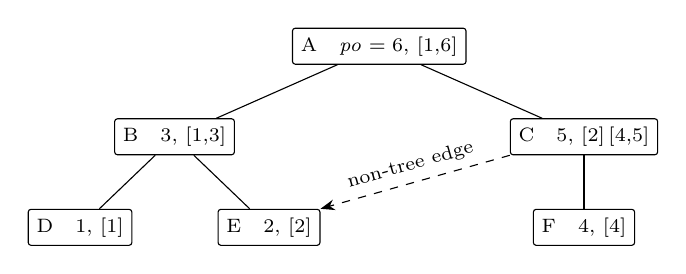
\begin{tikzpicture}[font=\scriptsize,level distance=1.15cm,
  every node/.style={draw,rounded corners=1pt,inner sep=3pt,fill=white},
  level 1/.style={sibling distance=5.2cm},level 2/.style={sibling distance=2.4cm}]
\node (a) {A\quad$\mathit{po}=6$,\ [1,6]}
  child { node (b) {B\quad$3$,\ [1,3]} child { node (d) {D\quad$1$,\ [1]} } child { node (e) {E\quad$2$,\ [2]} } }
  child { node (c) {C\quad$5$,\ [2]\,[4,5]} child { node (f) {F\quad$4$,\ [4]} } };
\draw[-{Stealth[length=1.8mm]},dashed] (c.south west) -- node[draw=none,fill=none,midway,above,sloped]{non-tree edge} (e.north east);
\end{tikzpicture}
\caption{A DAG in which $E$ has two parents, $B$ and $C$. The spanning forest keeps
$E$ under $B$; the dashed edge is outside it. Each node shows its postorder number
and its interval set. $C$ needs two intervals: its own tree interval $[4,5]$ and
$[2]$, the label of $E$.}
\end{figure}

\subsection{Three ways to answer a type query}

Under RDFS, \code{?x a C} means ``$x$ has a type at or below $C$''.

\begin{center}
\begin{tabular}{@{}p{2.1cm}p{3.6cm}p{5.2cm}@{}}
\toprule
Strategy & Extra stored & One query costs \\
\midrule
Rewrite & nothing & one POS scan per class below $C$ \\
Materialize (\cref{ch:inference}) & a type triple per ancestor of each type & one POS scan \\
Intervals & one key per type triple & one range scan per interval of $C$ \\
\bottomrule
\end{tabular}
\end{center}

The interval index stores \code{(po(type), instance)} once per type triple. An
instance insert adds one key. The price is that labels change when the hierarchy
does, so OntoDB rebuilds them in $O(n+m)$ instead of maintaining them
(Agrawal et al.\ describe incremental maintenance with gaps; it is not built). A
related idea, numbering a tree in preorder and postorder so that axes become
regions of a plane, was used for XML by Grust \cite{grust2002}.

\begin{decision}{Ids stay first-seen; labels are a separate index}
\dpart{Choice} The dictionary keeps handing out dense ids in first-seen order. The
postorder labels live in their own B+ tree, \code{(label, member, 0)}, which
OntoDB rebuilds when the hierarchy changes.
\dpart{Alternatives} Renumber the dictionary so ids follow the hierarchy; then the
existing SPO, POS, and OSP trees would give subtree scans with no extra index.
\dpart{Why} Ids are stored in three permutations, in the log, and in snapshots.
A hierarchy edit would renumber all of them. A label is derived data.
\dpart{Cost} One more small tree, and a rebuild after the hierarchy changes.
\end{decision}

\section{Vector indexes}

The second question needs vectors. OntoDB keeps one unit-length float vector
per term id, so cosine similarity is a dot product. Embeddings come from
outside; a small sentence model on a CPU embeds the 38\,092 Gene Ontology names
in under a minute. OntoDB stores and searches them; it does not run the model.

\begin{description}[leftmargin=1.2em]
\item[Flat.] Score every vector: $O(nd)$ and exact. With 8-bit scalar
quantization (one scale per vector, $s = \max|x|/127$) a stored coordinate is
off by at most $s/2$, so for a unit query a score is off by at most
$(s/2)\sqrt d$, at a quarter of the memory.
\item[IVF] (inverted file \cite{jegou2011}). Cluster the vectors into $L$ lists
with $k$-means \cite{arthur2007}. A query scores the $L$ centroids, then only the
$p$ nearest lists: cost $Ld + p(n/L)d$, minimal at $L=\sqrt{pn}$, where it equals
$2d\sqrt{pn}$. OntoDB stores each list as a range of a B+ tree: key
\code{(list, row, 0)}, so a list is a prefix scan and an insert is a tree
insert.
\item[Product quantization.] Cut a vector into $m$ pieces and replace each by the
index of its nearest of 256 learned centers: $m$ bytes per vector. A query builds
$m$ tables of 256 dot products ($256d$ work), and a stored code scores as the sum
of $m$ table entries. That equals the dot product with the decoded vector exactly,
so all the error is in the stored side.
\item[HNSW] (hierarchical navigable small world \cite{malkov2020}). A layered
proximity graph searched greedily: memory $O(nM)$, the slowest to build, usually
the best recall for a given time, and no worst-case bound.
\end{description}

\begin{decision}{IVF lists are B+ tree ranges}
\dpart{Choice} A posting list is the set of keys \code{(list, row, 0)} in a
B+ tree of the same kind as the triple indexes.
\dpart{Alternatives} A separate array per list in memory, as FAISS keeps them
\cite{johnson2021}.
\dpart{Why} The tree already pages, caches, and latches; an insert or delete is a
tree operation; a list is a prefix scan, the access path OntoDB is built around.
\dpart{Cost} The vectors themselves are still fetched by row from the vector store,
one random access per candidate.
\end{decision}

\section{Filtering a vector search by a class}

A hybrid query asks for the $k$ terms nearest $t$ that lie under class $C$. Let
$s = |\mathrm{subtree}(C)|/n$.

\begin{description}[leftmargin=1.2em]
\item[Pre-filter.] Resolve $C$ to its members first (one range scan per
interval), then score only those, exactly: about $s\,n\,d$ work. Best when $s$ is
small.
\item[Post-filter.] Ask the index for more than $k$, keep those under $C$ (a
membership test is a binary search over $C$'s intervals; no scan), and ask for
four times as many until $k$ remain. If the filter were independent of the
similarity one would need about $k/s$ candidates, so it fails when $s$ is small.
\item[In-index filter.] Resolve $C$, then give the index the set as a mask: IVF
skips list entries outside it, HNSW still crosses masked nodes to stay connected
but never returns them \cite{patel2024}.
\end{description}

In an ontology the filter and the vectors are \emph{not} independent: the names
of a class's descendants are close to the class and to each other. A query from
inside $C$ finds most of its neighbors inside $C$, so post-filtering works far
better than $k/s$ predicts; a query from outside finds almost none, and it works
far worse. \Cref{sec:semantic-measure} measures both.

\section{Why not an ART with sibling links}

An adaptive radix tree \cite{leis2013} orders keys by byte, so its range scan is a
\emph{lexical} range scan: every label that starts with \code{rub}. That is a real
query, and the ART is good at it, but it is the same one-dimensional order as the
B+ tree, and \cref{lem:bandwidth} applies unchanged.

Sibling links on an ART's leaves are possible. Path compression and node growth
never move a leaf. Lazy expansion does: an insert that meets a leaf turns it into
an inner node and puts a \emph{copy} of the leaf under it, so a link that pointed
at the old object now points at an inner node. Every insert must also find its
sorted neighbors, a partial descent, and concurrent inserts must latch both. A B+
tree has the link for free: a leaf is a page, and a split is local. The
usual alternative is a stack-based iterator: no link, climb and descend a stack of
\code{[node, keys, next child]}, which pays pointer chasing between leaves and
costs nothing on insert. OntoDB's keys are three fixed-width
integers, which gives an ART little prefix to compress, so the B+ tree stays.

\paragraph{Pessimistic and optimistic prefixes.} Path compression stores a node's
shared prefix. \emph{Pessimistic} storage keeps the bytes in the node, so a
descent compares them and fails at the first wrong byte; the cost is
variable-length storage. \emph{Optimistic} storage keeps only the length: the
descent skips those bytes and the full key is checked once, at the leaf. Nodes are
smaller, and a wrong path is found late. For a range scan the difference is in the
seek. To find the first key at or above $\mathit{lo}$ the seek must know whether a
whole subtree lies below or above $\mathit{lo}$. With stored bytes it decides at the
node; with skipped bytes it must load a key from the subtree and compare. The
upper bound needs no jumping: a second seek finds the first key past $\mathit{hi}$.
The only binary search in a scan is over the sorted edge bytes of one node.

\section{What it costs}
\label{sec:semantic-measure}

These measurements are on the Gene Ontology (release 2026-07-26, without
obsolete terms: 38\,092 classes, 57\,456 \code{is\_a} edges), with the term names
embedded by a 22-million-parameter sentence model on a CPU. LUBM and a set of
synthetic instances give the type queries something to run on. Everything is
one thread on an Apple M2 Pro, and \code{benchmarks/semantic/run.sh} reproduces
it; the full tables are in \code{benchmarks/semantic/results.md}.

\paragraph{Does an order put neighbors together?} For 2\,000 random terms, the
ten nearest by cosine; \cref{tab:semantic-order} gives the share within $\pm W$
positions.

\begin{table}[ht]
\centering\small
\begin{tabular}{@{}lrrrrr@{}}
\toprule
Order & median gap & $\pm$100 & $\pm$1000 & $\pm$5000 \\
\midrule
dictionary id (first seen) & 1739 & .211 & .284 & .438 \\
hierarchy postorder & 45 & .377 & .561 & .735 \\
label, alphabetical & 1749 & .334 & .408 & .558 \\
random & 10823 & .005 & .049 & .242 \\
\bottomrule
\end{tabular}
\caption{Share of the ten nearest neighbors found within $\pm W$ positions.}
\label{tab:semantic-order}
\end{table}

The postorder of the hierarchy is the best order, and far better than first-seen
ids: the nearest neighbor is a median of 45 positions away instead of 1\,739. It
still finds only 38\% of the ten within 100 positions, and 56\% within 1\,000, as
\cref{lem:bandwidth} says to expect. First-seen ids are not random either: the
Gene Ontology minted its ids in related batches, so id order carries locality that
belongs to the file, not to the engine. A term's neighbor is a parent or child in
12\% of cases and within two \code{is\_a} steps in 32\%, in a two-step
neighborhood of 45 terms (0.12\% of all terms): the hierarchy is informative about
meaning without being sufficient.

\paragraph{Intervals.} The Gene Ontology needs 76\,570 intervals for 38\,092
classes: 2.01 per class on average, 598~KiB in all, at most 741 for one class,
inside the bound of \cref{lem:size} (19\,368). Materializing the subclass closure
would store 393\,448 ancestor pairs. Whether $d$ is below $c$ takes 27~ns, 29 times
faster than a search up the parents. The descendants of a class with 1\,000 or more
subclasses take 101 range scans and 40 page reads, against 3\,304 scans and 694
pages for one scan per class.

\paragraph{Three ways to answer \code{?x a C}.} On 200\,000 synthetic entities over
the Gene Ontology's classes (495\,552 triples):

\begin{center}
\small
\begin{tabular}{@{}lrrr@{}}
\toprule
Strategy & triples & file (MiB) & load (s) \\
\midrule
rewrite & 495\,552 & 63.6 & 5.1 \\
intervals & 495\,552 & 72.9 & 5.3 \\
materialize & 4\,017\,973 & 309.5 & 180.3 \\
\bottomrule
\end{tabular}
\end{center}

Materializing stores 8.1 times the triples and takes 36 times as long to load. For
a class with 1\,000 or more subclasses a query reads 265 pages with intervals, 182
with the materialized store, and 12\,803 by rewriting (48 times more than
intervals). All three return the same answers on every class sampled. On LUBM(1),
whose hierarchy has 43 classes and little depth, the three are within a factor of
about two; intervals have little to save where the hierarchy is shallow.

\begin{decision}{Intervals instead of a materialized closure for type queries}
\dpart{Choice} A query for the instances of a class is one range scan per interval
of the class, over an index of \code{(label of type, instance)}.
\dpart{Alternatives} Materialize the entailed type triples (\cref{ch:inference});
rewrite into one scan per subclass.
\dpart{Why} On a deep, wide hierarchy the interval index costs 15\% more space
instead of 4.9 times as much, loads in 5 seconds instead of 180, and reads within 1.8
times of the materialized store's pages.
\dpart{Cost} The labels are rebuilt when the hierarchy changes, and only
\code{subClassOf} is understood: no \code{subPropertyOf}, \code{domain}, or
\code{range}. A materialized closure handles those rules with the same machinery
and an interval index does not.
\end{decision}

\paragraph{Vector indexes.} 38\,092 vectors of 384 floats; recall@10 against the exact
answer, time per query on one thread.

\begin{center}
\small
\begin{tabular}{@{}llrrr@{}}
\toprule
Index & setting & recall & $\mu$s & MiB \\
\midrule
flat float32 & exact & 1.000 & 2\,238 & 55.8 \\
flat PQ $m{=}48$ & codes only & 0.778 & 819 & 1.7 \\
IVF $L{=}512$ & nprobe 16 & 0.929 & 255 & 56.5 \\
IVF $L{=}512$ & nprobe 64 & 0.976 & 928 & 56.5 \\
HNSW $M{=}16$ & $ef$ 10 & 0.993 & 44 & 59.7 \\
HNSW $M{=}16$ & $ef$ 40 & 0.997 & 108 & 59.7 \\
\bottomrule
\end{tabular}
\end{center}

HNSW dominates on this data: 0.993 recall at 44~$\mu$s, 51 times faster than the
exact scan. A word on that baseline: the first run scored with a plain dot-product
loop, which a compiler may not vectorize without \code{-ffast-math}, and the exact
scan took 8.3~ms. With eight independent accumulators it takes 2.2~ms, and a
speed-up over ``exact'' is only as meaningful as the exact baseline is fast. IVF
lists stored in the B+ tree cost about 2.7 times as much per scored row as a flat
scan (157~ns against 59~ns): a decoded key and a random read of the vector, the
price of lists that page and update like the triples. Product quantization is for
memory; re-ranking its best 100 exactly gives 0.998 recall, but needs the floats.

\paragraph{The ten nearest terms under a class.} \Cref{tab:semantic-hybrid} gives
time and recall for five subtree sizes, with a query from inside the class.

\begin{table}[ht]
\centering\small
\begin{tabular}{@{}lrrrrr@{}}
\toprule
Members of $C$ & $\le$10 & 11--100 & 101--1000 & 1001--5000 & $>$5000 \\
\midrule
pre-filter & 3 & 9 & 62 & 292 & 1\,404 \\
post-filter, HNSW & 37\,553 & 1\,739 & 427 & 70 & 68 \\
masked HNSW & 16\,653 & 15\,846 & 1\,150 & 183 & 105 \\
masked IVF & 1\,253 & 111 & 104 & 124 & 161 \\
auto & 3 & 9 & 59 & 269 & 95 \\
\bottomrule
\end{tabular}
\caption{Microseconds per query, query inside $C$. Pre-filter, post-filtered and masked HNSW are exact at these sizes; masked IVF has recall 0.95 to 1.00.}
\label{tab:semantic-hybrid}
\end{table}

Pre-filtering through the interval index is exact and the fastest up to about a
thousand members, by factors from 1.7 to more than 10\,000. The filter is
correlated with the vectors: of the unfiltered top 100 neighbors of a term inside
$C$, 4\% to 72\% lie under $C$, and for a term outside it 0\% to 12\%. The
independence estimate $k/s$ is therefore wrong in both directions, and
post-filtering IVF recalls 0.07 of the right answers on the smallest classes for a
query outside them. A masked HNSW search wins above 5\,000 members (105~$\mu$s inside
and 900~$\mu$s outside, exact). One more lesson: resolving the members into a bitmap
before a masked search cost 560~$\mu$s of a 669~$\mu$s query, while testing each
touched row's label against the intervals, one binary search, cost nothing extra
and brought it to 105~$\mu$s. \code{kAuto} takes the exact path up to 4\,096 members
and a masked HNSW search above, and is within a factor of about two of the best
strategy everywhere but one cell.

\begin{decision}{Resolve small classes, mask large ones}
\dpart{Choice} Up to 4\,096 members: resolve the members by range scans and score
them exactly. Above: search HNSW with a predicate, ``the row's label lies in an
interval of $C$''.
\dpart{Alternatives} Always post-filter; always mask; always resolve.
\dpart{Why} Resolving is exact and fastest while a class is small. Post-filtering
fails for a query outside a small class. The threshold sits below the point where an
outside query makes masking slower than resolving (7\,000 to 25\,000 members) and
loses at most a factor of 3.8 where an inside query makes masking faster (about
1\,000).
\dpart{Cost} One threshold for both kinds of query; a class of 1\,001 to 5\,000
members queried from inside runs 3.8 times slower than it could.
\end{decision}


\begin{status}
Built (plan 14.1--14.9): class labels, the interval indexes, the vector store,
flat, IVF, and HNSW indexes, hybrid search, the shell commands
(\code{\textbackslash hindex}, \code{\textbackslash under},
\code{\textbackslash vload}, \code{\textbackslash vindex},
\code{\textbackslash similar}), and the benchmarks of this chapter
(\code{benchmarks/semantic/}). Vectors live in memory, not in buffer pool pages,
and the structures are not updated by inserts: they are rebuilt.
\end{status}

\begin{checkyourself}
\item Why does a sort order of dictionary ids not put similar classes next to each other? What would have to be true of the input file for it to?
\item Use \cref{lem:bandwidth} to bound how far apart two neighbors must be in the best order of a $10 \times 10$ grid.
\item Give the postorder labels and the interval sets of the diamond $D \sqsubseteq B, C \sqsubseteq A$ for a spanning forest that keeps $D$ under $B$.
\item A class has 5 non-tree edges below it. How many intervals can it have at most, and why?
\item When is pre-filtering better than post-filtering for a class filter, and when is it not?
\item Why can post-filtering work better than the independence estimate $k/s$ says, in an ontology?
\item What does a seek for a lower bound have to do differently if prefixes are stored optimistically?
\end{checkyourself}

\section*{Further reading}
Agrawal, Borgida, and Jagadish \cite{agrawal1989} on interval labelling of
transitive relationships; Jégou, Douze, and Schmid \cite{jegou2011} on
inverted files and product quantization; Malkov and Yashunin \cite{malkov2020}
on HNSW; Patel et al.\ \cite{patel2024} on filtered vector search; Pan, Wang, and
Li \cite{pan2024} for a survey of vector database systems; Leis, Kemper, and
Neumann \cite{leis2013} on the adaptive radix tree.


\part{Transactions}
\chapter{Transactions and Isolation}
\label{ch:transactions}

A \term{transaction} is a group of reads and writes that the database treats as
one unit. Transactions let an application reason about one operation at a time,
even though many run concurrently and any of them may be interrupted by a crash.

\section{ACID}

\begin{description}[leftmargin=1.2em]
\item[Atomicity.] All of a transaction's writes happen, or none do. A transaction that aborts, or is cut off by a crash, leaves no trace. (Provided by the log: \cref{ch:wal,ch:aries}.)
\item[Consistency.] A transaction takes the database from one valid state to another, where ``valid'' is defined by the application's invariants. The engine helps with constraints, but consistency is mostly the application's promise.
\item[Isolation.] Concurrent transactions do not see each other's intermediate states; the result is as if they ran in some order. (Provided by concurrency control: \cref{ch:concurrency}.)
\item[Durability.] Once a commit is acknowledged, its effects survive any later crash. (Provided by the log and \code{fsync}.)
\end{description}

\section{Schedules and serializability}

A \term{schedule} is the interleaved order in which the operations of
concurrent transactions actually execute. A schedule is \term{serializable} if
its effect equals that of \emph{some} serial order of the same transactions.
Serializability is the gold standard of isolation: the application cannot tell
that concurrency happened.

Two operations \term{conflict} if they come from different transactions, touch
the same item, and at least one is a write. A schedule is
\term{conflict-serializable} if it can be turned into a serial one by swapping
adjacent non-conflicting operations. The test is a graph: draw an edge
$T_i \to T_j$ for every pair of conflicting operations where $T_i$'s comes
first. The schedule is conflict-serializable exactly when the graph has no cycle.

\section{Anomalies}

Weaker isolation admits specific bad interleavings. Naming them is the clearest
way to define the isolation levels \cite{berenson}.

\begin{description}[leftmargin=1.2em]
\item[Dirty read.] $T_2$ reads a value $T_1$ wrote but has not committed. If $T_1$ aborts, $T_2$ read data that never existed.
\item[Non-repeatable read.] $T_1$ reads an item, $T_2$ changes it and commits, and $T_1$ reads it again and sees a different value.
\item[Phantom.] $T_1$ reads the set of items matching a condition (``every student''), $T_2$ inserts a new matching item and commits, and $T_1$ repeats the query and sees an extra row.
\item[Lost update.] Both transactions read a counter, both add one, both write: one increment disappears.
\end{description}

\section{Isolation levels}

\begin{table}[ht]
\centering
\begin{tabular}{@{}lccc@{}}
\toprule
Level & Dirty read & Non-repeatable read & Phantom \\
\midrule
Read uncommitted & possible & possible & possible \\
Read committed & --- & possible & possible \\
Repeatable read & --- & --- & possible \\
Serializable & --- & --- & --- \\
\bottomrule
\end{tabular}
\caption{The SQL standard's levels, defined by the anomalies they forbid.}
\label{tab:isolation}
\end{table}

Berenson et al.\ \cite{berenson} showed that defining levels by these phenomena
alone is ambiguous, and that real systems' levels (notably snapshot isolation,
which forbids all three but admits a ``write skew'') do not fit the table
cleanly. The table remains the right first mental model.

\begin{keyidea}
Isolation is a dial, not a switch. Lower levels allow more concurrency and
specific anomalies; serializable allows none. Each level is defined by what it
forbids, and each forbidden anomaly corresponds to a specific lock held for a
specific time (\cref{ch:concurrency}).
\end{keyidea}

\begin{ontodb}[: transactions]
Every shell statement is its own transaction unless \code{\textbackslash begin}
opens an explicit one, ended by \code{\textbackslash commit} or
\code{\textbackslash abort}. Isolation is a setting,
\code{\textbackslash set isolation ru|rc|rr|ser}, defaulting to read committed.
The isolation contract is written as executable schedules: twelve specs, each a
scripted interleaving of two sessions with expectations such as ``session 2 is
blocked'', ``the read returns Dana'', or ``session 2 is aborted''. They cover
dirty reads, non-repeatable reads, lost updates, lock upgrades, two deadlock
shapes, write--write conflicts, locks released on abort, and phantoms.

In a persistent database today, each update statement (or \code{\textbackslash
load}) is one atomic, durable transaction (\cref{ch:durability}).
\end{ontodb}

\begin{status}
Statement-level atomicity and durability run today. Explicit multi-statement
transactions and isolation levels are plans 7.2 to 7.6.
\end{status}

\section*{Further reading}
Gray and Reuter \cite{grayreuter}; Berenson et al.\ \cite{berenson}; Petrov
\cite{petrov}, chapter 5.

\chapter{Concurrency Control}
\label{ch:concurrency}

Isolation levels say \emph{what} must hold; concurrency control is \emph{how}.
This chapter covers locking, the approach OntoDB takes: two-phase locking,
multi-granularity locks, deadlock handling, phantoms, and the separate problem
of protecting the B+ tree's own structure.

\section{Two-phase locking}

A transaction takes a \term{shared} (S) lock to read an item and an
\term{exclusive} (X) lock to write it. S is compatible with S; X is compatible
with nothing. \term{Two-phase locking} (2PL) adds one rule: a transaction may
not acquire any lock after it has released one. Its life has a growing phase
and a shrinking phase.

2PL guarantees conflict-serializability: the order in which transactions reach
their \term{lock point} (the moment they hold all their locks) is an equivalent
serial order.

Plain 2PL has a flaw. If $T_1$ releases an X lock before committing and $T_2$
reads the value, then $T_1$ aborts, $T_2$ has read a value that never existed,
and must abort too: a \term{cascading abort}. \term{Strict 2PL} holds every
X lock until commit or abort, which rules this out.

\begin{keyidea}
Exclusive locks are held to the end of the transaction at every isolation
level, because releasing one early lets others see a write that may still be
undone. The isolation levels differ only in how long \emph{shared} locks are
held, and whether ranges are locked.
\end{keyidea}

\begin{table}[ht]
\centering
\begin{tabular}{@{}ll@{}}
\toprule
Level & Shared locks \\
\midrule
Read uncommitted & none \\
Read committed & released at the end of each statement \\
Repeatable read & held until commit \\
Serializable & held until commit, plus range or predicate locks against phantoms \\
\bottomrule
\end{tabular}
\caption{Isolation levels as locking rules, given strict 2PL for writes.}
\end{table}

\section{Locking at several granularities}

Locking every triple is precise but expensive for a query that reads the whole
store; locking the whole store is cheap but serializes everything. Gray et al.\
\cite{gray1976} let a transaction choose its granularity, using
\term{intention} locks on the coarser levels: before locking a key in S, take
IS (``intends to share something below'') on the index and on the database.

\begin{table}[ht]
\centering
\begin{tabular}{@{}lccccc@{}}
\toprule
Held \textbackslash{} Requested & IS & IX & S & SIX & X \\
\midrule
IS  & yes & yes & yes & yes & --- \\
IX  & yes & yes & --- & --- & --- \\
S   & yes & --- & yes & --- & --- \\
SIX & yes & --- & --- & --- & --- \\
X   & --- & --- & --- & --- & --- \\
\bottomrule
\end{tabular}
\caption{Multi-granularity lock compatibility. SIX is S on the whole node plus the intention to write below it.}
\label{tab:compat}
\end{table}

The point of intention locks: a transaction that wants to lock a whole index in
S can check one lock on the index, instead of every key below it, because any
writer below must already hold IX there.

\section{Deadlock}

$T_1$ holds a lock $T_2$ wants, and $T_2$ holds a lock $T_1$ wants: both wait
forever. Engines either \emph{prevent} deadlock (order locks, or abort on
conflicts by timestamp, as in wait--die and wound--wait) or \emph{detect} it:
maintain a \term{waits-for graph} with an edge $T_i \to T_j$ when $T_i$ waits for
a lock $T_j$ holds, find a cycle, and abort one transaction in it, the
\term{victim}. Choosing the youngest transaction (the one that has done the least
work) is a common and deterministic policy.

\section{Phantoms}

Repeatable read locks the triples a transaction read. A phantom is a triple it
did \emph{not} read, because it did not exist yet; no lock covers it. Preventing
phantoms needs a lock on what \emph{could} match, not on what does:

\begin{description}[leftmargin=1.2em]
\item[Predicate locks] lock the query's condition itself. Precise, but testing whether two predicates overlap is expensive in general \cite{eswaran}.
\item[Key-range (next-key) locks] lock the gap between index keys, so an insert into the scanned range must wait. Practical, and natural on a B+ tree.
\end{description}

\section{Latches are not locks}

A B+ tree split rewrites several pages at once. Even a single-transaction
engine with many threads must stop two threads from splitting the same page at
the same time. That protection is a \term{latch}: a short-term reader--writer
mutex on a page, held for the duration of one tree operation, never for a
transaction. Locks protect \emph{logical contents} for transactional isolation;
latches protect \emph{physical structure} for thread safety.

The classic latch protocol for B+ trees is \term{crabbing}: latch the child,
and release the parent if the child is \emph{safe}, meaning it cannot split (for
an insert) or merge (for a delete) as a result of this operation. A thread
therefore holds latches only on the part of the path a structure change could
reach. An \term{optimistic} variant takes shared latches down to the leaf,
latches only the leaf exclusively, and restarts pessimistically if the leaf
turns out to need a split. Lehman and Yao's B-link tree \cite{lehmanyao} goes
further and lets readers run without latching the path at all, by following
right-links when a split has moved their key.

\section{The alternative: multiversion concurrency}

Locking makes readers and writers wait for each other. \term{Multiversion
concurrency control} (MVCC) keeps old versions of items, so a reader sees a
consistent snapshot as of its start time and never waits for a writer. Writers
still conflict with writers. The cost is storing old versions and cleaning them
up once no reader can need them. Most modern systems use MVCC with snapshot
isolation by default.

\begin{ontodb}[: concurrency control]
OntoDB uses strict 2PL with five lock modes on three granularities: the
database, an index (\code{"spo"}, \code{"pos"}, \code{"osp"}), and a key, with
FIFO grant order and in-place upgrades that do not jump ahead of waiters. A
blocked shell session prints why it is waiting, for example
\code{session 2 waiting: X lock held by txn 5}. A background thread builds the
waits-for graph and aborts the \emph{youngest} transaction in each cycle (the
larger id), so deadlock outcomes are deterministic and testable. Serializable
adds one phantom mechanism, chosen and documented in the code. B+ tree
operations use latch crabbing, and the whole feature runs under
ThreadSanitizer. MVCC is a deliberate future comparison, not part of the plan.
\end{ontodb}

\begin{status}
Concurrency control is plans 7.1 to 7.6: crabbing, transactions, the lock
manager, isolation, deadlock detection, and phantoms. The isolation harness
already exists and checks itself.
\end{status}

\section*{Further reading}
Gray et al.\ \cite{gray1976}; Eswaran et al.\ \cite{eswaran}; Lehman and Yao
\cite{lehmanyao}; Bayer and Schkolnick \cite{bayerschkolnick}; Petrov
\cite{petrov}, chapters 5 and 6.


\part{Recovery}\label{part:recovery-ref}
\chapter{Logging and the Write-Ahead Rule}
\label{ch:wal}

The buffer pool steals and does not force (\cref{ch:buffer}). So at the moment of
a crash, the disk can hold changes from transactions that never committed, and
can lack changes from transactions that did. The \term{log} is what lets the
engine repair both. This chapter explains what goes in it, and the one rule that
makes it trustworthy.

\section{The failure model}

\begin{description}[leftmargin=1.2em]
\item[Transaction failure.] A transaction aborts: a deadlock victim, a constraint violation, or the user's choice. Its effects must be removed.
\item[System failure.] The process or machine stops. Memory is lost; the disk survives. Committed work must reappear; uncommitted work must vanish.
\item[Media failure.] The disk is lost. Only a backup or a replica helps; it is outside the scope of the log alone.
\end{description}

The log handles the first two. It is an append-only file of \term{log records},
each describing one change, written sequentially, which is the access pattern
storage handles best.

\section{Undo and redo}

An update record carries enough to apply the change again (\term{redo}) and to
reverse it (\term{undo}). For a page-oriented engine that might be the bytes
before and after; for a triple store it can be logical: ``insert triple
(5, 7, 9)'', whose undo is ``delete (5, 7, 9)''.

Every record has a \term{log sequence number} (LSN), increasing, unique, and
often simply the record's byte offset in the log. Records of one transaction are
chained by a \term{prevLSN} field, so the engine can walk a transaction's history
backward when it must undo it.

Every page stores a \term{pageLSN}: the LSN of the last logged change applied to
it. The pageLSN is how recovery knows whether a logged change already reached
the page on disk: if pageLSN $\ge$ the record's LSN, it did.

\section{The write-ahead rule}

\begin{keyidea}
\textbf{Write-ahead logging (WAL).} (1) A page may be written to disk only after
every log record describing a change to it is durable: flush the log up to the
page's pageLSN first. (2) A transaction commits only when its commit record, and
therefore all its earlier records, are durable.
\end{keyidea}

Rule 1 makes steal safe: if an uncommitted change reaches the disk, its undo
information is already in the log. Rule 2 makes no-force safe: if a committed
change has not reached the disk, its redo information is already in the log.
Between them, every possible state of the disk after a crash can be repaired.

\begin{figure}[ht]
\centering
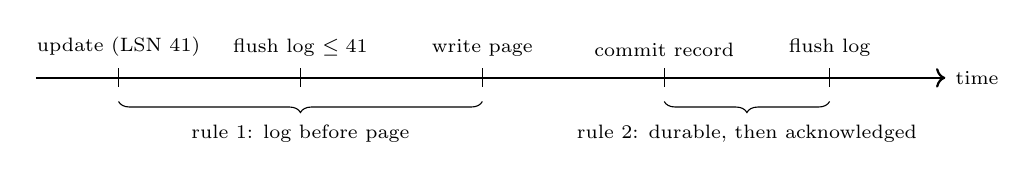
\begin{tikzpicture}[font=\scriptsize,x=1.05cm]
\draw[thick,->] (0,0) -- (11,0) node[right]{time};
\foreach \x/\l in {1/update (LSN 41),3.2/flush log $\le 41$,5.4/write page,7.6/commit record,9.6/flush log}{
  \draw (\x,0.12) -- (\x,-0.12); \node[above,align=center] at (\x,0.15) {\l};}
\draw[decorate,decoration={brace,amplitude=4pt,mirror}] (1,-0.3) -- (5.4,-0.3) node[midway,below=5pt]{rule 1: log before page};
\draw[decorate,decoration={brace,amplitude=4pt,mirror}] (7.6,-0.3) -- (9.6,-0.3) node[midway,below=5pt]{rule 2: durable, then acknowledged};
\end{tikzpicture}
\caption{The two orderings the write-ahead rule imposes.}
\label{fig:wal}
\end{figure}

\section{Making commits cheap: group commit}

Rule 2 means every commit waits for an \code{fsync} of the log. If each commit
issued its own \code{fsync}, throughput would be bounded by the device's
\code{fsync} rate. \term{Group commit} lets commits that arrive while a flush is
in progress share the next one:

\begin{lstlisting}[language=pseudo]
function Commit(txn):
  lsn = Append(commit record for txn)       // into the in-memory log buffer
  wait until persistentLSN >= lsn           // a background flusher wakes us

flusher loop:
  wait until someone asked, or a short interval passes
  batch = swap out the log buffer
  write(batch); fsync()                     // one fsync for many commits
  persistentLSN = last LSN in batch; wake all waiters
\end{lstlisting}

Under concurrency, the number of \code{fsync} calls grows much more slowly than
the number of commits. A single client still pays the full latency of one flush.

\section{When a record is damaged}

A crash can interrupt the last write to the log, leaving a \term{torn} record:
fewer bytes than its header promises. Bit rot or a misbehaving device can damage
a record whose bytes are all present. Robust logs detect both with two fields in
every record header: its \textbf{length}, so a short record is recognized, and a
\textbf{checksum} over its bytes, so a damaged one is. PostgreSQL, RocksDB, and
InnoDB all put a CRC on every log record. A recovery procedure then has a
policy choice, discussed in \cref{ch:durability}: stop at the first bad record
and keep everything before it, or refuse to start.

\begin{ontodb}[: log records and the log manager]
Every OntoDB log record has this layout (native byte order):

\begin{lstlisting}
u32 size       whole record, header included
u32 crc32c     over every byte after this field
u8  type       begin | commit | abort | update | clr | checkpoint | term | page
i64 lsn, i64 txn_id, i64 prev_lsn
then, by type:
  update       i32 page_id, u8 is_insert, u64 subject, u64 predicate, u64 object
  clr          the update fields, then i64 undo_next
  checkpoint   u32 n, then n active transaction ids
  term         u64 term_id, u32 n, then n bytes of canonical spelling
  page         i32 page_id, then the page's bytes after its pageLSN
\end{lstlisting}

The checksum is CRC-32C, the same checksum PostgreSQL, RocksDB, and InnoDB use.
A short buffer raises an ordinary storage error (a torn write), while a record
whose bytes are present but wrong raises a distinct corruption error, so the two
cases can be handled differently. LSNs start at 1; reopening a log continues
after its last valid record.

The log manager appends records to an in-memory buffer and a background thread
performs group commit; a test runs four threads committing twenty times each and
requires fewer \code{fsync}s than commits. A failed \code{fsync} is reported,
never retried, for the reason in \cref{ch:pages}.
\end{ontodb}

\begin{decision}{Length and CRC-32C in every record}
\dpart{Choice} Each record starts with its size and a CRC-32C over the rest. A
short record raises a storage error (a torn write); a full-length record with a
wrong checksum raises a distinct corruption error.
\dpart{Alternatives} No checksum; a plain CRC-32; a faster non-cryptographic
hash such as xxHash.
\dpart{Why} A crash leaves a torn tail, and the two cases deserve different
handling. CRC-32C has hardware instructions on x86 and ARM and is what
PostgreSQL, RocksDB, and InnoDB use.
\dpart{Cost} Eight bytes of header per record, and a checksum per append and per
read.
\end{decision}

\begin{decision}{LSNs are counters, not byte offsets}
\dpart{Choice} An LSN is a 64-bit counter starting at 1. On open, the next LSN
is one past the larger of the snapshot's LSN and the last valid record.
\dpart{Alternatives} Use the record's byte offset in the log, as ARIES and
PostgreSQL do, so an LSN locates its record directly.
\dpart{Why} A checkpoint of the memory database empties the log file. A counter
keeps increasing across that truncation, so ``skip records at or below the
snapshot's LSN'' stays correct; an offset would restart at zero.
\dpart{Cost} Finding a record by LSN needs a scan, not a seek.
\end{decision}

\begin{decision}{A failed \code{fsync} is fatal}
\dpart{Choice} When a log flush fails, the error is reported and the commit is
not acknowledged. The flush is never retried.
\dpart{Alternatives} Retry until it succeeds.
\dpart{Why} After a failed \code{fsync}, the kernel may have dropped the dirty
pages and cleared the error, so a retry that succeeds can still have lost the
data (\cref{ch:pages}).
\dpart{Cost} A transient device error stops the database instead of being
ridden out.
\end{decision}

\section{What a page record holds}

Rule 1 needs every change to a page to be logged before the page can be
written, and redo needs enough in each record to put the change back. There
are three common answers to ``what does the record hold''. \term{Physical}
logging records the bytes: a whole page image, or a byte range and its new
contents. \term{Logical} logging records the operation (``insert key $k$
into the SPO index''), and redo performs it again. \term{Physiological}
logging, which ARIES and most disk engines use, is a mix: the record names one
page (physical) and describes an operation on that page (logical), such as
``insert this key at slot 7 of page 12''.

Each choice moves work around. Page images are the simplest to redo (copy the
bytes) and need no knowledge of what is on the page, but they are large.
Logical records are small, but redo must run the operation against a structure
that may itself be damaged, which is why engines that log logically above the
page level still log pages physically below it.

\section{Changes that span pages}

A B+ tree split changes three pages: the old leaf loses its upper half, a new
leaf receives it, and the parent gains a separator. Each page gets its own
record. Suppose the log reaches the disk with the records for the two leaves
but not the parent's, and then the machine stops. Redo faithfully rebuilds
both leaves, and the parent still has no pointer to the new one. A full scan,
which walks the leaf chain, finds every key; a point lookup for a key in the
new leaf descends to the old leaf and misses. Nothing in the log is wrong, yet
the tree is.

The write-ahead rule is about single pages, so it cannot prevent this. A
multi-page change needs its own rule: its records must reach the log all
together or not at all. Systems get there in different ways:

\begin{description}[leftmargin=1.2em]
\item[Nested top actions (ARIES).] Log the split's page changes with undo information, then a dummy CLR that marks the split complete. If the crash comes before the dummy CLR, undo reverses the half-done split page by page.
\item[Mini-transactions (InnoDB).] Hold every latch the change took until it is finished, then append all its records to the log buffer in one step.
\item[Tolerate the half state (PostgreSQL).] B-link trees give every page a right link and a high key, so a search that lands on the old leaf can follow the right link. A split missing its parent pointer is legal, and the next writer that notices finishes it.
\end{description}

\begin{ontodb}[: page images and page groups]
OntoDB logs physically, by whole page. When a write guard on a page it changed
is released, still latched, the buffer pool appends a page record holding the
page's bytes after the pageLSN and sets the pageLSN to that record's LSN
(\code{BufferPoolManager::LogPageWrite}). Every page written through a guard
is covered by this one path: B+ tree nodes, tree headers, and the catalog.
Triple changes get a logical update record too, appended before the
statement changes any page; undo uses those (\cref{ch:aries}).

A tree \code{Insert} or \code{Remove} opens a \code{PageGroup} before its
first latch and closes it after its last. While a group is open, the log
manager writes nothing from the group's first LSN onward, so the flusher can
cut the log only between groups. The buffer pool, choosing a victim, passes
over any dirty page whose pageLSN is still held back, since writing it would
break rule 1. A test stops a tree at each named crash point inside a split or
a merge, flushes everything the log allows, copies the files, and checks that
redo yields a sound tree that holds either every key from before the
operation or every key from after it. Without page groups, all seven cases
fail.
\end{ontodb}

\begin{decision}{Whole page images, not physiological records}
\dpart{Choice} A page record carries the whole page after its pageLSN. Redo
copies it when the record is newer than the page.
\dpart{Alternatives} Physiological records, ``insert key $k$ at slot $i$ of
page $p$'', as ARIES and InnoDB use; byte-range diffs.
\dpart{Why} Redo needs to know nothing about the layout of a leaf, an internal
node, a header, or the catalog, so one short loop redoes them all, and a bug
in a page's code cannot also be a bug in its redo. The guard already knows
when a page changed; it does not know how.
\dpart{Cost} About 4 KB per page per operation. One triple touches at least
three trees, so it logs at least three pages, where its logical update
record is a few dozen bytes. A real engine would log diffs, or log a full
image only the first time a page changes after a checkpoint, as PostgreSQL's
full-page writes do.
\end{decision}

\begin{decision}{Page groups hold back the log, not the latches}
\dpart{Choice} A group marks its first LSN. The log does not flush past it, and
the pool does not evict a dirty page the group holds back, until the group
ends.
\dpart{Alternatives} Nested top actions with before-images and undo of an
unfinished split; InnoDB's mini-transaction, which keeps every page latched
until the end; B-link trees that accept a half split.
\dpart{Why} No before-images, no recovery pass for unfinished splits, and no
change to latching. Holding latches longer would have broken the tree's rule
that siblings are latched left to right, since a merge releases a page to
latch its left sibling.
\dpart{Cost} While any group is open, every later record waits too, so a
commit that arrives during a split waits for it. A group's pages cannot be
evicted, so the pool must hold more frames than the largest split touches. A
pool so small that every unpinned frame is held back cannot find a victim.
\end{decision}

\begin{status}
Log records (plan 8.1), the log manager with group commit (plan 8.2), and the
write-ahead rule with pageLSNs set on every change (plan 8.3) run. The rule
applies wherever a buffer pool is given a log manager: the recovery tests and
the crash harness. The shell's indexed backend is a temporary file and runs
without a log, and \code{ontodb <dir>} opens the memory database of
\cref{ch:durability}.
\end{status}

\begin{checkyourself}
\item State the two write-ahead rules, and say which buffer-pool policy each one makes safe.
\item A page has pageLSN 40. Recovery reads an update record for it with LSN 35. Redo it or skip it?
\item Ten sessions commit within one millisecond. Without group commit, how many \code{fsync}s? With it, at least how many?
\item A log's last record has a valid header claiming 60 bytes, and only 41 are in the file. Torn or corrupt? What if all 60 are there but the checksum fails?
\item Why does OntoDB number LSNs with a counter rather than a byte offset?
\item A split logs the old leaf, the new leaf, and the parent, in that order. Only the first two records reach the disk before a crash. After redo, which reads still work, and which fail?
\item Why may the buffer pool not evict a dirty page whose pageLSN is newer than the log's flushable LSN, even though it may wait for an ordinary log flush?
\item OntoDB logs whole page images. Name one thing this makes simpler and one thing it makes more expensive.
\end{checkyourself}

\section*{Further reading}
Mohan et al.\ \cite{aries}, sections 1--3; Gray and Reuter \cite{grayreuter},
chapters 9--10; Petrov \cite{petrov}, chapter 5.

\chapter{ARIES}
\label{ch:aries}

ARIES (Algorithm for Recovery and Isolation Exploiting Semantics), published by
Mohan, Haderle, Lindsay, Pirahesh, and Schwarz in 1992 \cite{aries}, is the
recovery algorithm behind most disk-based database systems. It supports steal
and no force, fine-grained locking, and partial rollbacks, and it recovers
correctly even if the system crashes again \emph{during} recovery. Its central
idea fits in three words: \textbf{repeat history, then undo}.

\section{The data structures}

\begin{description}[leftmargin=1.2em]
\item[Log records] as in \cref{ch:wal}: LSN, transaction id, prevLSN, and type-specific fields.
\item[pageLSN] on every page: the LSN of the last change applied to it.
\item[Transaction table] for every active transaction: its status and \term{lastLSN}, the LSN of its most recent record.
\item[Dirty page table] for every page dirty in the buffer pool: its \term{recLSN}, the LSN of the first record that made it dirty since it was last read from disk. Any change to the page before recLSN is already on disk.
\item[Compensation log records (CLRs)] written when a change is undone. A CLR describes the undo, and carries \term{undoNextLSN}: the next record of that transaction still to undo.
\end{description}

\section{Checkpoints}

Without checkpoints, recovery would read the log from the beginning of time. A
\term{fuzzy checkpoint} writes the transaction table and the dirty page table
into the log without stopping the system or forcing any pages, and records the
checkpoint's LSN in a well-known place. Recovery then starts from the last
checkpoint: the tables in it tell analysis everything that happened before.

\section{Pass 1: Analysis}

Scan the log forward from the last checkpoint, rebuilding the two tables as of
the crash:

\begin{itemize}
\item On any record of a transaction not in the table, add it. Update its lastLSN.
\item On a commit, mark it committed; on an end record, remove it.
\item On an update or CLR for a page not in the dirty page table, add the page with recLSN = this LSN.
\end{itemize}

At the end, every transaction still in the table without a commit is a
\term{loser}. The \term{redoLSN} is the smallest recLSN in the dirty page table:
no earlier change can be missing from disk.

\section{Pass 2: Redo}

Scan forward from redoLSN, and reapply every update and every CLR, for winners
and losers alike, unless the change is provably already on disk:

\begin{lstlisting}[language=pseudo]
for each update or CLR record r, from redoLSN forward:
  if r.page not in dirty page table:          skip   // page was clean at the crash
  if dirtyPageTable[r.page].recLSN > r.lsn:   skip   // flushed after r
  fetch page
  if page.pageLSN >= r.lsn:                   skip   // r already on the page
  apply r to the page; page.pageLSN = r.lsn
\end{lstlisting}

Redo \textbf{repeats history}: it brings the database to exactly its state at
the crash, uncommitted changes included. That sounds wasteful, but it makes undo
simple: undo now starts from a precise, known state, and can use the same
logical operations that a normal abort uses.

\section{Pass 3: Undo}

Undo the losers, newest change first, across all of them at once:

\begin{lstlisting}[language=pseudo]
toUndo = { lastLSN of each loser }
while toUndo is not empty:
  r = record with the largest LSN in toUndo; remove it
  if r is a CLR:
    if r.undoNextLSN exists: add r.undoNextLSN to toUndo
    else: write an end record for r.txn
  else if r is an update:
    undo r; write CLR(undoNextLSN = r.prevLSN)
    if r.prevLSN exists: add r.prevLSN to toUndo
    else: write an end record for r.txn
\end{lstlisting}

\begin{keyidea}
A CLR is redone but never undone. If the system crashes during undo, the next
recovery redoes the CLRs (history repeats), then follows their undoNextLSN
pointers past everything already undone. Recovery work is therefore bounded no
matter how many times the system crashes during recovery.
\end{keyidea}

\section{A worked example}

Two transactions run. $T_1$ commits; $T_2$ does not. The buffer pool happened
to write page P2 (stealing $T_2$'s uncommitted change), but never wrote P1.

\begin{center}
\begin{tabular}{@{}rlll@{}}
\toprule
LSN & Transaction & Record & prevLSN \\
\midrule
10 & $T_1$ & update P1 & --- \\
20 & $T_2$ & update P2 & --- \\
30 & $T_1$ & commit & 10 \\
40 & $T_2$ & update P1 & 20 \\
\multicolumn{4}{@{}l}{\emph{crash.} On disk: P1 has pageLSN 0; P2 has pageLSN 20.} \\
\bottomrule
\end{tabular}
\end{center}

\paragraph{Analysis.} $T_1$ committed; $T_2$ is a loser with lastLSN 40. The
dirty page table is \{P1: recLSN 10, P2: recLSN 20\}, so redoLSN is 10.

\paragraph{Redo.} LSN 10 on P1: pageLSN 0 $<$ 10, so redo; P1's pageLSN becomes
10. LSN 20 on P2: pageLSN 20 $\ge$ 20, so skip; the stolen write already put it
there. LSN 40 on P1: pageLSN 10 $<$ 40, so redo; pageLSN becomes 40. The
database is now exactly as it was at the crash, including $T_2$'s two changes.

\paragraph{Undo.} toUndo = \{40\}. Undo LSN 40 on P1, write CLR 50 with
undoNextLSN 20. Undo LSN 20 on P2, write CLR 60 with no undoNextLSN, then an end
record for $T_2$. $T_1$'s change survives; $T_2$ left no trace.

If the system had crashed right after CLR 50, the next analysis would find $T_2$
with lastLSN 50; redo would reapply CLR 50; undo would read CLR 50, jump straight
to LSN 20, and never undo LSN 40 a second time.

\section{Structure changes: nested top actions}

A B+ tree split moves keys between pages. Suppose $T$ inserts a key, which
splits a leaf, and later aborts. Undoing ``the split'' would be wrong: another
transaction may have committed an insert into the new leaf since then. The
split is a change to the \emph{structure}, which is valid regardless of who
caused it; only the \emph{logical} insert belongs to $T$.

ARIES logs a split as a \term{nested top action}: the split's page records,
followed by a dummy CLR whose undoNextLSN points to the record just before the
split. Redo replays the split like any other change. Undo, following the dummy
CLR, skips over it. The logical ``insert key $k$'' is logged separately, and its
undo is the logical ``delete key $k$'', performed wherever that key now lives,
which is why undo in ARIES is logical while redo is physical.

\begin{ontodb}[: ARIES]
OntoDB's page-based recovery follows this chapter: steal and no force,
page-oriented redo, logical undo of triples, CLRs that are redone and never
undone, and B+ tree splits logged as redo-only nested top actions with the
triple insert logged separately. On open, recovery prints one line per pass
(\code{analysis}, \code{redo}, \code{undo}). The bar for the feature is a crash
harness that kills the process at random points (including named crash points
inside splits and between a log flush and a page write) and compares the
reopened store with an oracle that replayed only acknowledged commits:
\code{scripts/crashtest --seeds 200} must pass.
\end{ontodb}

\begin{decision}{A blocking checkpoint first (planned)}
\dpart{Choice} The page store's \code{\textbackslash checkpoint} may pause
updates while it writes the checkpoint record; the comment above
\code{Checkpoint} names which kind it is.
\dpart{Alternatives} ARIES's fuzzy checkpoint, which never stops the system.
\dpart{Why} A blocking checkpoint is easy to reason about and enough to bound
recovery. Fuzzy checkpointing is an optimization to add once the three passes
are correct.
\dpart{Cost} Updates stall for the length of the checkpoint.
\end{decision}

\begin{decision}{Recovery is tested against an oracle}
\dpart{Choice} A crash harness kills the process at random points and at named
crash points, reopens the store, and compares it with an oracle that applied
only acknowledged commits. The harness is itself tested on deliberately broken
stores.
\dpart{Alternatives} Hand-written recovery scenarios only.
\dpart{Why} The bugs in recovery live in interleavings nobody thinks to write.
Many random crash points find them; a harness that catches a planted lost
commit proves it can.
\dpart{Cost} Slow tests, and failures that need a seed to reproduce.
\end{decision}

\begin{status}
The log record types used here, including CLRs and checkpoints, exist and
serialize (plan 8.1). Abort by the log, checkpoints, the three passes, and the
crash test are plans 8.4 to 8.7, after the buffer pool and B+ tree. The crash
harness already detects a lost commit and a surviving uncommitted write on
deliberately faulty test stores.
\end{status}

\begin{checkyourself}
\item In the worked example, suppose the pool had also written P1 after LSN 40. What does redo do now, and what does undo do?
\item Why does ARIES redo the losers' changes, only to undo them right after?
\item The system crashes after CLR 60 but before $T_2$'s end record. What does the next recovery do?
\item Why is a B+ tree split never undone, even when the transaction that caused it aborts?
\item What do the dirty page table's recLSNs let redo skip?
\end{checkyourself}

\section*{Further reading}
Mohan et al.\ \cite{aries}, the whole paper; Ramakrishnan and Gehrke
\cite{cowbook}, chapter 18, for a gentler walkthrough; Petrov \cite{petrov},
chapter 5.

\chapter{Durability in Practice}
\label{ch:durability}

ARIES is the general answer for a page-based engine. A simpler engine can make a
simpler choice and still be correct. OntoDB's persistent databases, which run
today, are such a design: an in-memory database made durable by a
\textbf{snapshot} plus a \textbf{logical, redo-only write-ahead log}. This
chapter explains the design through the ideas of the previous chapters, because
every choice in it is one of those ideas in a smaller form.

\section{Where it sits in the steal/force table}

The database lives entirely in memory; the files are its durable copy. Nothing
is ever written to the data files except a whole snapshot, and a snapshot is
taken only between statements, when every change in memory is committed. In the
terms of \cref{tab:stealforce}:

\begin{itemize}
\item \textbf{No steal.} Uncommitted changes never reach the snapshot. So recovery never needs to \emph{undo} anything on disk.
\item \textbf{No force.} A commit does not rewrite the snapshot; it appends to the log. So recovery must \emph{redo} committed changes made since the last snapshot.
\end{itemize}

No steal plus no force is the \emph{redo-only} cell: the log needs redo
information and nothing else, and recovery is a single forward pass.

\begin{keyidea}
Choosing a cell of the steal/force table chooses the recovery algorithm. Steal
and no force need undo and redo (ARIES). No steal and no force need only redo.
The price of no steal is that all uncommitted state must fit in memory, which an
in-memory database accepts by definition.
\end{keyidea}

\section{Logical logging}

Page-based ARIES logs \emph{physical} or \emph{physiological} changes: this page,
these bytes, or this page, this slot. The memory database has no pages, so it
logs \emph{logical} operations: ``insert triple (18, 9, 4)''. Logical records are
small and independent of storage layout, and they are safe here only because
there is no partially written page that could make a logical operation
ambiguous on replay.

Ids in those records must mean the same terms after a restart, so the log also
carries the dictionary: a \term{term record} for each spelling the first time a
transaction uses it.

\section{One statement, one transaction}

\begin{enumerate}
\item The statement runs against a \term{recording store}, a decorator around the real store that remembers every triple it actually changed.
\item The log receives \textbf{begin}, a \textbf{term} record for each new spelling, one \textbf{update} per changed triple, and \textbf{commit}.
\item The commit is forced (\cref{ch:wal}) before the shell prints the result.
\end{enumerate}

If the statement fails part way, the recording store's changes are undone in
memory, in reverse order, and nothing it needs reaches the log. A statement that
changed nothing logs nothing.

\begin{figure}[ht]
\centering
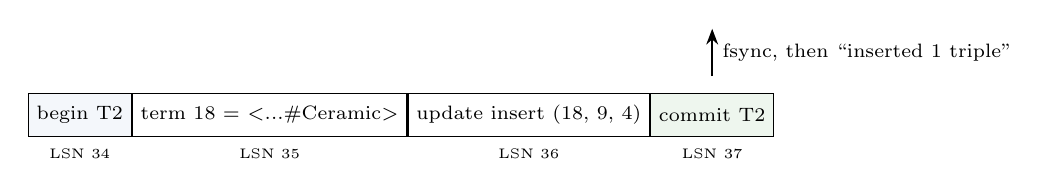
\begin{tikzpicture}[font=\scriptsize,rec/.style={draw,minimum height=0.55cm,inner sep=3pt,fill=white}]
\node[rec,fill=boxbg] (b) {begin T2};
\node[rec,right=0pt of b] (t) {term 18 = \textless...\#Ceramic\textgreater};
\node[rec,right=0pt of t] (u) {update insert (18, 9, 4)};
\node[rec,right=0pt of u,fill=statusbg] (c) {commit T2};
\foreach \n/\l in {b/34,t/35,u/36,c/37}{\node[below=1pt of \n,font=\tiny] {LSN \l};}
\draw[arrow] ([yshift=6pt]c.north) -- node[right]{fsync, then ``inserted 1 triple''} ++(0,0.6);
\end{tikzpicture}
\caption{The log records of one \code{INSERT DATA} in a persistent database.}
\end{figure}

\section{Recovery}

Opening a database directory:

\begin{enumerate}
\item Load the snapshot, if there is one: every term in id order, then every triple.
\item Scan the log and stop at the first record that is torn or fails its checksum (\cref{ch:wal}).
\item Skip records at or below the snapshot's LSN; the snapshot already contains them.
\item Apply \emph{every} term record in order, whatever its transaction did: the dictionary only grows, and a term no committed triple uses is invisible.
\item Apply update records only for transactions that have a commit record, in log order.
\end{enumerate}

Step 5 is the whole of ``undo'' in a redo-only design: an uncommitted
transaction's records are simply never applied.

\section{Checkpoints as atomic snapshots}

A checkpoint writes the full state to \code{snapshot.tmp}, \code{fsync}s it,
\code{rename}s it over \code{snapshot}, \code{fsync}s the directory, and then
empties the log. Each step is safe to crash after:

\begin{center}
\begin{tabular}{@{}ll@{}}
\toprule
Crash after & On reopen \\
\midrule
writing \code{snapshot.tmp} & old snapshot, full log: nothing lost \\
the rename & new snapshot, old log: records at or below its LSN are skipped \\
emptying the log & new snapshot, empty log \\
\bottomrule
\end{tabular}
\end{center}

This is the log-structured idea of \cref{ch:lsm} with a single level: an
append-only log, periodically compacted into one sorted image.

\section{Damaged logs: recovery modes}

When the scan in step 2 stops early, there are two defensible policies, named
after RocksDB's WAL recovery modes:

\begin{description}[leftmargin=1.2em]
\item[Point in time] (the default). Keep every transaction before the bad record, truncate the log there, and report how many bytes were discarded. A torn final record is the normal shape of a crash, and this is the right answer for it; a transaction whose commit is after the damage is treated as uncommitted, exactly as a crash would.
\item[Absolute consistency] (\code{--strict}). Refuse to open, so an operator can inspect the files before anything is truncated.
\end{description}

A damaged snapshot always refuses to open: it has no valid prefix to fall back
to.

\section{Verification}

Detecting damage early is the other half of durability. The \code{\textbackslash
verify} command follows the tradition of PostgreSQL's \code{pg\_amcheck},
MySQL's \code{CHECK TABLE}, and RocksDB's \code{VerifyChecksum}: it changes
nothing and reports four checks, one line each.

\begin{lstlisting}
snapshot: ok (lsn 37, 18 terms, 15 triples)
wal: ok (0 records, 0 bytes)
replay: matches the live database (15 triples)
invariants: ok (no duplicate triples, every id in the dictionary)
verify: ok
\end{lstlisting}

The replay check is the strongest: it rebuilds the database from the two files
into a fresh store and compares it with the one in memory. If they differ, the
files would not reproduce what the user sees.

\section{Testing a recovery design}

A recovery path that is never exercised does not work. OntoDB tests this one with
\term{crash points}: named places in the code, such as just before a commit
record is appended and just after a snapshot is renamed, where a test can make
the operation stop as if the process died. Scenario tests then reopen the
directory and check what survived: a crash before commit leaves no trace, a crash
after the snapshot rename does not replay records twice, a torn tail keeps the
committed prefix, a flipped byte in the middle of the log drops everything after
it, and a tampered log fails verification.

\begin{ontodb}[: what runs]
All of this chapter runs today: start the shell as \code{ontodb mydb}.
\code{\textbackslash load} and every update are durable transactions,
\code{\textbackslash checkpoint} writes a snapshot, \code{\textbackslash log}
prints the decoded log, \code{\textbackslash verify} checks the files, and
\code{\textbackslash crash} exits without flushing, to try recovery by hand.
Seventeen scenario tests cover the cases above, and they pass under
AddressSanitizer, UndefinedBehaviorSanitizer, and ThreadSanitizer.

When the indexed store arrives, the same log records, log manager, and group
commit carry over; what changes is that pages can be stolen, so recovery gains
undo, pageLSNs, and the three passes of \cref{ch:aries}.
\end{ontodb}

\begin{decision}{Terms replay whatever their transaction did}
\dpart{Choice} On recovery, every term record is applied in order, even if its
transaction never committed; update records apply only for committed
transactions.
\dpart{Alternatives} Replay terms only for committed transactions.
\dpart{Why} Ids are dense, and each term record carries the id it was given.
If an aborted transaction's term were skipped, every later term would land on a
different id than the log recorded. A term no committed triple uses is
invisible.
\dpart{Cost} Aborted transactions can leave unused terms behind.
\end{decision}

\begin{decision}{Point-in-time recovery by default}
\dpart{Choice} A damaged log is truncated at the first bad record, and the
database opens with everything before it, reporting what was dropped.
\code{--strict} refuses to open instead.
\dpart{Alternatives} Strict by default; or skip the bad record and continue.
\dpart{Why} A torn final record is the ordinary result of a crash, and the
right response is to open. Skipping a bad record would apply later
transactions on top of a missing one.
\dpart{Cost} Damage in the middle of the log silently loses every later commit
apart from the report, which is why \code{\textbackslash verify} exists.
\end{decision}

\begin{checkyourself}
\item Why can the memory database's log omit undo information?
\item A crash happens after the snapshot rename but before the log is emptied. Which records does reopen apply?
\item A transaction logs a term record for id 19 and then fails. A later committed transaction logs id 20. Why must replay still apply the term for 19?
\item When would you choose \code{--strict} over point-in-time recovery?
\item Why is the replay check of \code{\textbackslash verify} stronger than checking checksums alone?
\end{checkyourself}

\section*{Further reading}
Gray and Reuter \cite{grayreuter} on redo-only logging; DeWitt et al.\
\cite{dewitt1984} on recovery for main-memory databases; the RocksDB WAL
recovery-mode documentation \cite{rocksdbwal}.

\chapter{From Memory to Pages}
\label{ch:pagestore}

OntoDB now has two complete recovery designs. The memory database of
\cref{ch:durability} is redo-only: no steal, a logical log, and snapshots. The
page store of \cref{ch:aries} steals pages, logs page images, and recovers
with ARIES, but only tests open it. This chapter is about the step that joins
the second design to the shell, so that \code{ontodb <dir>} keeps its data on
pages. Most of the work is not new algorithms; it is deciding what a directory
\emph{is}, what opening one does, and which operations get which kind of log
record. Those decisions are where real systems differ.

\section{What is in a directory}

A database directory must say which design wrote it, because the two have
incompatible files. The memory database keeps \code{snapshot} and \code{wal};
the page store keeps \code{db}, the database file of \cref{ch:pages}, and its
own \code{wal}. A one-line \code{format} file names the store and its version,
\code{pages 1}, much as PostgreSQL keeps a \code{PG\_VERSION} file in every
data directory.

\begin{center}
\begin{tabular}{@{}ll@{}}
\toprule
Directory holds & Opens as \\
\midrule
\code{format} = \code{pages 1} & a page store \\
\code{snapshot}, no \code{format} & a memory database, as today \\
\code{format} naming another store or version & refused, saying which \\
nothing & a new page store (or memory, with \code{--memory}) \\
\bottomrule
\end{tabular}
\end{center}

Refusing an unknown format is the important row. A newer OntoDB that changes
the page layout must not be opened by an older one that would misread it, and
the cheapest protection is a version number checked before any page is read.

\begin{decision}{A format file names the store (planned)}
\dpart{Choice} New directories get \code{format} with the store and version;
a directory without it but with a \code{snapshot} is a memory database.
\dpart{Alternatives} Detect the store from which files exist; or put the
version in the database file's header page.
\dpart{Why} Detection by file names breaks the day both designs share a name,
and a header page cannot describe a store that has no pages. A separate file
is read before anything else and is trivial to inspect.
\dpart{Cost} One more file to create atomically with the others.
\end{decision}

\section{Opening is recovery}

On the memory path, opening means loading a snapshot and replaying the log.
On the page path, opening a directory runs all of \cref{ch:aries}, in an order
that matters:

\begin{enumerate}
\item \textbf{Cut a torn tail.} Scan the log and truncate it at the first record
that is incomplete or fails its checksum. The recovery modes of
\cref{ch:durability} apply: point in time truncates and reports; \code{--strict}
refuses.
\item \textbf{Analysis and redo.} Rebuild the transaction table and the dirty
page table, then repeat history from the smallest recLSN, so every page is as
it was at the crash, uncommitted changes included.
\item \textbf{Open the catalog, the dictionary, and the indexes.} Only now are
the pages that describe them trustworthy, since redo has brought them up to
date.
\item \textbf{Undo.} Roll back the loser transactions, writing compensation
records, exactly as an abort does.
\end{enumerate}

Step 3 sits between redo and undo for a reason. Redo is physical: it needs
page ids and bytes, not trees. Undo of an index change is logical, ``remove
this key from that tree'', because a split may have moved the key to another
page since it was inserted; logical undo needs the tree, and the tree needs
its root page, which the catalog names.

\begin{keyidea}
Redo works on pages and needs nothing above the buffer pool. Undo works on
structures and needs the access methods. Recovery opens the engine layer by
layer, in that order.
\end{keyidea}

\section{Statements log on pages}

On a page directory the transaction manager is given the log manager, and from
then on the machinery of \cref{ch:wal,ch:aries} runs for every statement:
each page change logs a record, commit forces the log, and abort undoes by the
log. The dictionary's pages are pages like any other, so a new term is covered
by the page records of the term heap and the dictionary tree; there is no
separate term record as on the memory path. A term added by a transaction that
then aborts stays in the dictionary, for the same reason as there: ids are
handed out densely, and an unused term is invisible.

The test for this step is blunt and sufficient: commit a triple, kill the
process before any page is written, reopen, and find the triple. Only the log
can have put it there.

\section{Loading: one record per triple, or one per load}

\code{\textbackslash load} of a large file is one transaction, and it is where
the two obvious logging designs diverge most:

\begin{description}[leftmargin=1.2em]
\item[Log every change.] Each inserted triple dirties leaf pages of three
trees, and each change is logged. Simple and uniform: a load is just a big
transaction. The log grows with the data, roughly three page records per
triple until pages fill, and the load runs at the speed of logging.
\item[Minimal logging.] Build the trees bottom-up from sorted input
(\cref{ch:btree}'s bulk load), write every page to the file, force the file,
and log one record that names the load. Undo of the load is ``drop the new
trees''. SQL Server calls this minimal logging, and PostgreSQL, with
\code{wal\_level} set to \code{minimal}, skips the log for a table created in
the same transaction, for the same reason.
\end{description}

Minimal logging is only correct when the trees it builds start empty (or are
new trees swapped in at commit): there is nothing older on those pages for a
partial load to have damaged, so undo can discard them whole.

\begin{decision}{How a load is logged (planned, to be measured)}
\dpart{Choice} Decide between per-triple logging and minimal logging by
measuring both on LUBM(1): log bytes and load time. A crash during a load must
leave the database as it was before it, either way.
\dpart{Alternatives} The two above; or per-page images of the newly built
trees.
\dpart{Why} The answer depends on numbers this engine has not produced yet:
how much faster a bulk build is than three tree inserts per triple, and how
much log a load writes.
\dpart{Cost} Minimal logging needs empty target trees and forces every page
before commit; per-triple logging makes the log as large as the data.
\end{decision}

\section{Closing cleanly, and checkpoints}

A clean exit (\code{\textbackslash quit}, or end of input) writes every dirty
page, forces the log, and closes the file. The next open then finds nothing to
redo, and its summary says so; that is the cheapest test that the close was
clean. \code{\textbackslash checkpoint} runs the sharp checkpoint of
\cref{ch:aries} with every statement held out, because a sharp checkpoint must
not see a page change in the middle of being made. \Cref{ch:logkeep} replaces
it with a fuzzy one.

\section{Checking a page database}

\code{\textbackslash verify} keeps its promise of changing nothing and grows
three checks: every tree satisfies its invariants (\cref{ch:btree}); SPO, POS,
and OSP hold the same set of triples; and every id in them is in the
dictionary. The second check is the one specific to RDF: three indexes that
disagree return different answers depending on which one the optimizer
chooses, the worst kind of bug to find from the query side.

\section{Testing through the shell}

The crash harness of \cref{ch:aries} kills a store driven by test code. The
last step drives the real \code{Database} with SPARQL text on a page directory
and kills it between statements and at named crash points. Test-only options
make tree nodes tiny and the buffer pool small, so a short script splits,
merges, and steals pages constantly; otherwise a test database never leaves its
first page, and the hard paths never run.

\begin{status}
Planned, and next (plan 10.1--10.7). Today \code{ontodb <dir>} opens the memory
database of \cref{ch:durability}, and the page store's recovery runs only in
tests and in the crash harness.
\end{status}

\begin{checkyourself}
\item Why must an older OntoDB refuse to open a directory whose \code{format} names a newer version, rather than try?
\item Why are the catalog and the indexes opened after redo but before undo?
\item A transaction commits one \code{INSERT DATA}, and the process is killed before any page is written. Where does the reopened database find the triple?
\item Under what condition is minimal logging of a load correct, and what does undo of such a load do?
\item What does a clean close guarantee about the next open, and how can a test observe it?
\item Give a query whose answer depends on which of SPO, POS, or OSP the optimizer scans if the three disagree.
\end{checkyourself}

\section*{Further reading}
Mohan et al.\ \cite{aries} on logical undo of index changes; Gray and Reuter
\cite{grayreuter} on recovery-time ordering; the SQL Server documentation on
minimally logged operations \cite{sqlminimal}.

\chapter{Keeping the Log Small}
\label{ch:logkeep}

A write-ahead log only grows. Every commit appends, nothing removes, and a
database that runs for months would keep every record since its creation and
replay from the beginning of time on every crash. ARIES as described in
\cref{ch:aries} is correct but not yet livable. This chapter covers the three
pieces of housekeeping a long-lived page store needs: cutting the log after a
checkpoint, making page records smaller, and checkpointing without stopping
the world. Each is a statement about what recovery can still need, made
precise.

\section{What recovery still needs}

After a crash, ARIES redo starts at the smallest recLSN in the dirty page
table: the first change to any page not yet written. Undo walks back through
every loser transaction, so it needs each active transaction's records back
to its first one. Everything older than both is dead weight:
\[
\mathit{keep} \;=\; \min\Big(\min_{p\ \text{dirty}} \mathit{recLSN}(p),\ \ \min_{T\ \text{active}} \mathit{firstLSN}(T)\Big).
\]
A record below \textit{keep} describes a change already on disk, made by a
transaction already finished; no crash can need it. A checkpoint is the moment
these two minima are known and written down, which is why truncation follows a
checkpoint.

\begin{keyidea}
The log is a queue of obligations: redo for pages not yet written, undo for
transactions not yet finished. Its tail can be cut exactly at the oldest
obligation still open.
\end{keyidea}

\section{Cutting the log}

\Cref{ch:durability} empties its log after a snapshot, because the snapshot
holds everything. The page store cannot empty it: after a checkpoint, dirty
pages and active transactions still depend on records near the end. It keeps
the suffix from \textit{keep} on, and must do so without ever leaving a log
that recovers differently:

\begin{enumerate}
\item Write the records from \textit{keep} on to \code{wal.tmp}, and \code{fsync} it.
\item \code{rename} it over \code{wal}, and \code{fsync} the directory.
\end{enumerate}

\begin{center}
\begin{tabular}{@{}ll@{}}
\toprule
Crash after & On reopen \\
\midrule
writing \code{wal.tmp} & the old, full log: recovery as before \\
the rename & the cut log: same recovery, less to read \\
\bottomrule
\end{tabular}
\end{center}

LSNs are counters, not file offsets, so the records keep their LSNs and every
pageLSN on disk still points where it did. The file only needs to know the
LSN of its first record, which goes in its header.

\begin{decision}{Truncate by copying the tail (planned)}
\dpart{Choice} After a checkpoint, copy the needed suffix to a new file and
rename it over the log.
\dpart{Alternatives} A log made of fixed-size segment files, where truncation
deletes whole old segments, as PostgreSQL and InnoDB do.
\dpart{Why} One file keeps the log manager, the scanner, and the crash harness
as they are, and copying is cheap right after a checkpoint, when the suffix is
short.
\dpart{Cost} Copying a long suffix while a long transaction stays open; segment
files would avoid the copy and cost a directory of files to manage.
\end{decision}

\section{Torn pages and smaller page records}

\Cref{ch:aries} logs a page's full image with every change. That is simple and
robust, and it makes the log as large as the pages it touches: insert one
24-byte key into a 4\,KiB leaf, and the log grows by 4\,KiB.

Logging only the changed bytes is the obvious saving, and it has one hazard.
A page write is not atomic: the device may write some sectors of a page and
not others, leaving a \term{torn page} that is neither the old version nor the
new. Redo that applies a byte diff to a torn page produces garbage, because the
diff assumes the bytes around it are the old ones.

PostgreSQL's answer, \term{full-page writes}, is the one the plan adopts: the
\emph{first} change to a page after a checkpoint logs the page's full image,
and later changes until the next checkpoint log only the byte ranges that
differ from the page as it was when latched. Recovery starts from the
checkpoint, so for every page redo touches, it meets that page's full image
first and rebuilds the page whole, torn or not; every later diff then applies
to a known image.

\begin{center}
\begin{tabular}{@{}lr@{}}
\toprule
Inserting 100 keys into one leaf, one checkpoint & Log bytes \\
\midrule
Full image every change & $100 \times 4{,}096 \approx 410$\,KB \\
Full image first, then diffs (about 40 bytes each) & $4{,}096 + 99 \times 40 \approx 8$\,KB \\
\bottomrule
\end{tabular}
\end{center}

A diff must also say what it applies to. Redo applies a diff only to a page
whose pageLSN equals the LSN of that page's previous record, so a diff can
never land on the wrong version of the page.

\begin{decision}{Full image after a checkpoint, then diffs (planned)}
\dpart{Choice} Log a page's full image on its first change after each
checkpoint, and byte-range diffs for later changes.
\dpart{Alternatives} Full images always (today); diffs always, with a
doublewrite buffer to repair torn pages (InnoDB).
\dpart{Why} Torn pages are repaired from the log with no second write path,
and the log shrinks by roughly the ratio of a page to a change.
\dpart{Cost} Every checkpoint makes the next change to each page expensive
again, so checkpoints that are too frequent waste log; the benchmark measures
log bytes per triple before and after.
\end{decision}

\section{Fuzzy checkpoints}

The sharp checkpoint of \cref{ch:aries} holds every statement out, writes
every dirty page, and then records that nothing is dirty. Its pause grows with
the buffer pool. A \term{fuzzy checkpoint} writes no pages at all:

\begin{enumerate}
\item Append a \textbf{begin-checkpoint} record.
\item Copy the transaction table and the dirty page table, each page with its
recLSN, while transactions keep running, and append them in an
\textbf{end-checkpoint} record.
\item Force the log, and record the begin-checkpoint's LSN in a known place.
\end{enumerate}

Recovery's analysis pass starts from the begin-checkpoint record with the
tables the end record carries, and redo starts from the smallest recLSN in
the dirty page table. The checkpoint's copy of the tables may be slightly out
of date by the time it is written, which is why it is ``fuzzy'': analysis reads
the records between begin and end and brings the tables up to date, just as
it does for every record after the checkpoint.

Writing dirty pages becomes a background job (a page cleaner, in InnoDB's
terms) that keeps the smallest recLSN moving forward, so that redo after a
crash, and the log that truncation must keep, stay short. The two mechanisms
work together: the cleaner advances \textit{keep}, and the checkpoint records
where it is.

\begin{figure}[ht]
\centering
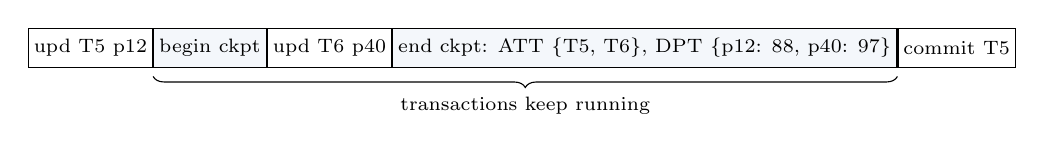
\begin{tikzpicture}[font=\scriptsize,rec/.style={draw,minimum height=0.5cm,inner sep=2pt,fill=white}]
\node[rec] (a) {upd T5 p12};
\node[rec,right=0pt of a,fill=boxbg] (b) {begin ckpt};
\node[rec,right=0pt of b] (c) {upd T6 p40};
\node[rec,right=0pt of c,fill=boxbg] (d) {end ckpt: ATT \{T5, T6\}, DPT \{p12: 88, p40: 97\}};
\node[rec,right=0pt of d] (e) {commit T5};
\draw[decorate,decoration={brace,mirror,amplitude=4pt}] ([yshift=-3pt]b.south west) -- node[below=4pt]{transactions keep running} ([yshift=-3pt]d.south east);
\end{tikzpicture}
\caption{A fuzzy checkpoint. No page is written; the end record carries the
active transactions and each dirty page's recLSN as they were seen.}
\end{figure}

\begin{status}
Planned (plan 11.1--11.3), after the page store reaches the shell
(\cref{ch:pagestore}). Today the log is never truncated, every page record is a
full image, and the checkpoint is sharp. The sharp checkpoint stays as an
option for comparison, and \code{benchmarks/logging/} will measure log bytes per
inserted triple, the checkpoint pause, and recovery time.
\end{status}

\begin{checkyourself}
\item The dirty page table holds p3 (recLSN 140) and p9 (recLSN 212); T7 is active with first LSN 120 and T8 with first LSN 300. From which LSN must the log be kept?
\item Why may truncation keep the old LSNs instead of renumbering from zero?
\item What goes wrong if redo applies a byte diff to a torn page, and how does a full image after each checkpoint prevent it?
\item Why does a diff record need the LSN of the page's previous record?
\item What does a fuzzy checkpoint write, and why may its tables be out of date when they reach the log?
\item Why does a fuzzy checkpoint make the page cleaner more important?
\end{checkyourself}

\section*{Further reading}
Mohan et al.\ \cite{aries} on fuzzy checkpoints and the dirty page table;
Gray and Reuter \cite{grayreuter} on log management; the PostgreSQL
documentation on WAL and full-page writes \cite{pgwal}.


\appendix
\chapter{A Map from Chapters to OntoDB}
\label{app:map}

Each chapter's ideas, the OntoDB plan items that implement them, and where the
code lives. Plan items are listed in the repository's \code{PLAN.md}; run
\code{scripts/check <feature>} to build and test one.

\begin{center}
\small
\begin{tabular}{@{}>{\raggedright\arraybackslash}p{3.4cm}>{\raggedright\arraybackslash}p{2.4cm}>{\raggedright\arraybackslash}p{6.6cm}@{}}
\toprule
Chapter & Plan items & Where \\
\midrule
\ref{ch:engine} The engine & 0.1, 0.3 & \code{tools/shell}, \code{src/common/database.cpp} \\
\ref{ch:pages} Pages & 1.1, 3.1 & \code{src/storage/disk}, \code{src/storage/page}, \code{src/storage/term} \\
\ref{ch:buffer} Buffer pool & 1.2--1.6 & \code{src/buffer}, \code{src/storage/page/page\_guard.cpp} \\
\ref{ch:btree} B+ trees & 2.1--2.7, 6.1--6.2 & \code{src/storage/index/b\_plus\_tree.cpp} \\
\ref{ch:rdf-indexing} Indexing RDF & 0.2, 3.2--3.6 & \code{src/storage/index/triple\_key.cpp}, \code{src/dictionary}, \code{src/catalog}, \code{src/store} \\
\ref{ch:lsm} LSM trees & --- & (contrast only) \\
\ref{ch:plans} Plans & 4.4--4.6 & \code{src/parser}, \code{src/binder}, \code{src/planner}, \code{src/execution} \\
\ref{ch:joins} Joins & 4.1--4.3, 5.1--5.5 & \code{src/execution/executors}, \code{src/execution/row\_merge.cpp}, \code{src/optimizer}, \code{src/stats} \\
\ref{ch:sparql} Beyond BGPs & 12.1--12.5 & (planned) \\
\ref{ch:inference} Inference & 13.1--13.5 & (planned) \\
\ref{ch:transactions} Transactions & 7.2, 7.4 & \code{src/concurrency}, \code{test/isolation/specs} \\
\ref{ch:concurrency} Concurrency & 7.1--7.6 & \code{src/concurrency}, B+ tree crabbing \\
\ref{ch:wal} Logging & 8.1--8.3 & \code{src/recovery/log\_record.cpp}, \code{src/recovery/log\_manager.cpp} \\
\ref{ch:aries} ARIES & 8.4--8.7 & \code{src/recovery}, \code{test/recovery}, \code{scripts/crashtest} \\
\ref{ch:durability} Durability & 9.1--9.7 & \code{src/recovery/durability.cpp}, \code{src/recovery/snapshot.cpp}, \code{test/durable} \\
\ref{ch:pagestore} Memory to pages & 10.1--10.7 & (planned, next) \\
\ref{ch:logkeep} Log housekeeping & 11.1--11.3 & (planned) \\
\bottomrule
\end{tabular}
\end{center}

The OntoDB manual (\url{https://lamng3.github.io/ontodb-docs/}) is the
companion to this book: it documents how to use each feature, while this book
explains why it is built the way it is.

\chapter{Answers}
\label{app:answers}

Short answers to the questions at the end of each chapter. Try a question
before reading its answer; most of them take one line of reasoning, and that
line is the point.

\newcommand{\answers}[2]{\section*{\cref{#1}: \nameref{#1}}\begin{enumerate}[label=#2.\arabic*,leftmargin=2.4em]}

\answers{ch:engine}{1}
\item (a) The B+ tree, an access method. (b) The buffer pool. (c) The optimizer.
\item It touches every layer: executors take locks on the keys they read and write, every page change is logged, and commit is decided at the interface. It cuts across the stack instead of sitting in it.
\item A five-way self-join of the triple table on the subject column, each pattern being a selection on that table, followed by a projection.
\item Only \code{Metal}. The stored triples say \code{Metal subClassOf Material}; \code{Alloy subClassOf Material} would have to be inferred, and OntoDB has no reasoner.
\end{enumerate}

\answers{ch:pages}{2}
\item At byte $37 \times 4096 = 151{,}552$. Pages are fixed-size, so the offset is arithmetic on the page id.
\item The index points at the record id, \emph{(page, slot)}. Compaction changes the offset stored in the slot, not the slot number.
\item No: it was only in the operating system's page cache. \code{fsync} on the file (and, for a new file, on its directory) makes it durable.
\item The kernel may already have dropped the dirty pages and cleared the error, so the second \code{fsync} ``succeeds'' with the data gone. The only safe response is to stop and recover from the log.
\item Zero is what unwritten memory and files contain. With $-1$ as the sentinel, a forgotten initialization shows up as an error instead of as a tree rooted at page 0, which is a legal page.
\item OntoDB refuses it: a term heap record must fit on one page (at most 4,076 bytes), so the term cannot be interned and the load fails as one transaction. PostgreSQL would compress it and, if still large, move it out of line into a TOAST table, leaving a pointer in the row.
\item Allocation grew the file, but the new length was never made durable (no \code{fsync} before the crash), while the log record that uses the page was forced. Redo reads the page past the end as zeros and reapplies the record; writing the page back grows the file.
\end{enumerate}

\answers{ch:buffer}{3}
\item It must be written back to disk (after the log is flushed up to its pageLSN, by the write-ahead rule) before the frame is reused.
\item At $t = 11$ the backward 2-distances are A: $11 - 8 = 3$, B: $11 - 3 = 8$, C: $11 - 7 = 4$. LRU-K evicts B.
\item X. Both have fewer than three accesses, so both have infinite distance, and the tie goes to the earliest oldest access: X's is at time 2, Y's at time 5. Recency does not enter until a frame has $K$ accesses.
\item A scan touches each page once; under LRU every scanned page becomes the most recent, so the scan pushes out the hot pages. With $K = 2$, a page touched once has infinite distance and leaves first. $K = 1$ is LRU.
\item Both steal cells. Under steal, an uncommitted change can reach the disk, and the log must be able to take it back.
\item The bytes just written: one thread runs requests in the order scheduled. With several I/O threads the read could run first and return the old page, unless requests for the same page were ordered some other way.
\item Until the first thread's read finishes: the pool's one latch is held across the I/O, and the single I/O thread would serialize the reads anyway.
\item It would write the very page the crash point was meant to keep off the disk, so the test could not observe the state a real crash leaves.
\item Once the pin is gone the pool may evict the frame and load a different page into it; a latch still held would then be a latch on someone else's page.
\item Page 7 is now resident (another page may have been evicted to make room), and its LRU-K history holds two recent accesses, so it has a finite, small distance and will be among the last to go.
\item That frame can never be evicted, so the pool is permanently one frame smaller; enough leaks and every frame is pinned and the next miss fails. Guards unpin exactly once at the end of their scope, and the tests check that nothing stays pinned.
\end{enumerate}

\answers{ch:btree}{4}
\item A 24-byte key plus a 4-byte child page id. $n$ keys separate $n + 1$ children, so the leftmost child has no key of its own, and storing slots uniformly simply leaves that key unused.
\item $300^3 = 2.7 \times 10^7 < 10^8 \le 300^4$, so four levels. The root and the roughly 300 pages below it are always cached, so a lookup costs about two reads.
\item The right (new) leaf, whose first key it is. Left in the left leaf, a key equal to the separator sits in the left child, which breaks the separator rule, and a search for 14 goes right.
\item Leaf keys are the data, and every key must stay in a leaf. Internal keys only route searches, so the middle one can move up and leave both halves.
\item Holding two leaves, and possibly a parent, can use up a small pool; with latches, two scans moving in opposite directions can deadlock.
\item A split would have to rewrite the parent pointer in every child that moved, up to 72 pages for one internal split. Without them, a structure change re-fetches parents remembered by id, which is safe only while one thread changes the tree; latch crabbing fixes that.
\item Two leaves of 85. A leaf of 1 would be below the minimum of 84 keys, so the last two leaves share their 170 keys evenly.
\item A full leaf splits into two half-full leaves, so random inserts leave leaves about two-thirds full, and each insert is a random descent. Bulk load writes full leaves sequentially.
\end{enumerate}

\answers{ch:rdf-indexing}{5}
\item 258 is \code{0x0102}. Big-endian: \code{00 00 00 00 00 00 01 02}; little-endian: \code{02 01 00 00 00 00 00 00}. Against 3 (\code{...00 03} and \code{03 00...}), big-endian puts 258 above 3, correctly; little-endian puts it below.
\item \code{(5, ?, ?)}: $[(5,0,0), (6,0,0))$. \code{(5, 7, ?)}: $[(5,7,0), (5,8,0))$.
\item With $n = 2$, the predicate overflows to 0 and the carry bumps the subject: $(6, 0, 0)$. With $n = 1$ and subject $2^{64}-1$, nothing is above the prefix, so the bound saturates to $(2^{64}-1, 2^{64}-1, 2^{64}-1)$.
\item Object bound: OSP. Subject and object bound: OSP, whose prefix is object then subject.
\item Otherwise one term gets two ids, and a join between loaded data and a query constant silently matches nothing. Example: a datatype written with a prefix, \code{"21"\^{}\^{}xsd:integer}, and the same datatype written as a full IRI must become one spelling.
\item Every operator would read that term as ``unbound'': a join would overwrite the slot from the other side, a scan would treat a constant as a variable, and the saturated upper bound could exclude a real key. The answers would be wrong without any error.
\item With SPO, POS, and OSP, every pattern shape is already a prefix of some index, so it is already a range scan; another order can only offer the same range sorted differently. That matters to an operator that wants its input in a particular order, such as a merge join on the object, or a sort that an index could avoid.
\item Range scans: subject bound; subject and predicate; all three; and none (the whole tree is the range). Subject and object bound is a subject range filtered by object. Predicate only, object only, and predicate with object are full scans with a filter.
\item The prefix scan on the hash returns both ids; the dictionary reads each candidate's spelling from the heap and returns the one that is equal. A collision costs an extra read, never a wrong answer.
\item A root moves whenever it splits or collapses; the header page absorbs those changes. The catalog changes only when an index is created or dropped.
\end{enumerate}

\answers{ch:lsm}{6}
\item An LSM tree: writes are sequential and batched. A B+ tree pays a random page write for each insert; the LSM tree pays later in compaction, and in read amplification.
\item Older versions of the key sit in immutable SSTables that are never edited. The tombstone shadows them until compaction drops both.
\item One wasted SSTable read. A Bloom filter never says ``absent'' for a present key.
\item Appending to the log is the write path, and a checkpoint rewrites the whole state as one sorted image, which is a compaction into a single level that discards the old log.
\end{enumerate}

\answers{ch:plans}{7}
\item \code{?s} is slot 0, \code{?name} slot 1, \code{?age} slot 2, in order of first appearance.
\item Rows can differ in slots that are not projected: two students with the same name are two scan rows but one projected row.
\item Ids are assigned in load order, not value order; \code{"10"} can have a smaller id than \code{"9"}. Sorting must compare values.
\item Volcano stops as soon as ten rows reach the root, doing only the join work that produced them. Materializing computes the entire join first, then keeps ten rows.
\item An empty pattern has exactly one solution, the empty binding, and that row is the identity for a join. Zero rows would make every join empty.
\end{enumerate}

\answers{ch:joins}{8}
\item Nested loop: $10^3 \times 10^6 = 10^9$ comparisons. Index nested loop: 1,000 prefix probes, each a root-to-leaf descent (mostly cached) plus the few matching triples.
\item When both inputs are large, no index makes a probe selective, and the build side fits in memory.
\item $(10^4 \times 10^3) / 10^6 = 10$. The q-error is $\max(10/1000,\ 1000/10) = 100$.
\item A join's estimate is built from its inputs' estimates, so their errors multiply: two inputs each off by 10 give an output off by up to 100.
\item \code{\textbackslash explain} prints the optimizer's plan. If the executor swapped algorithms at run time, the printed plan would not be the one that ran.
\end{enumerate}

\answers{ch:transactions}{9}
\item $r_1(A)$ before $w_2(A)$ gives $T_1 \to T_2$; $r_2(B)$ before $w_1(B)$ gives $T_2 \to T_1$. The graph has a cycle, so the schedule is not conflict-serializable.
\item $r_1(A)\, w_2(A)\, c_2\, r_1(A)$: $T_1$ reads two different values. Repeatable read is the first level that forbids it.
\item Validity is defined by the application's invariants, such as ``every student has a name''. The engine cannot know them; it provides atomicity, isolation, and durability, so that the application can keep them.
\item Both read $N$ and both insert a student they believe is number $N + 1$: an anomaly built on a phantom (write skew). It is possible at read uncommitted, read committed, and repeatable read. Serializable's range locks make one insert wait; if both hold the range in S and both want to insert, it is a deadlock, and the younger transaction is aborted.
\end{enumerate}

\answers{ch:concurrency}{10}
\item Plain 2PL may release an X lock in its shrinking phase, before commit; another transaction reads the value and must abort if the writer later aborts. Strict 2PL holds X locks until commit or abort, so no one reads an uncommitted write.
\item IS on the database and S on the \code{"spo"} index, with no key locks. Any writer below must hold IX on the index, and IX conflicts with S, so the one check on the index covers every key.
\item $T_5$, the younger (larger id).
\item A latch is a short mutex on a physical page for one operation; it protects a page's structure during a split. A lock is held for a transaction on a logical item, such as a triple key, and provides isolation.
\item For an insert, a child is safe if it is not full, so it cannot split. For a delete, it is safe if it is more than half full, so it cannot underflow.
\end{enumerate}

\answers{ch:wal}{11}
\item Rule 1: a page is written only after the log records for its changes are durable; this makes steal safe. Rule 2: a commit is acknowledged only after its commit record is durable; this makes no force safe.
\item Skip it: pageLSN $40 \ge 35$, so the change is already on the page.
\item Without group commit, ten. With it, as few as one, or two if a flush was already running when they arrived.
\item Short: a torn write. Full length with a bad checksum: corruption. In point-in-time mode, either one ends the valid prefix there.
\item A checkpoint of the memory database empties the log file. Byte offsets would restart at zero; a counter keeps increasing, so comparisons with the snapshot's LSN stay correct.
\end{enumerate}

\answers{ch:aries}{12}
\item Analysis is unchanged: the dirty page table still has P1 at recLSN 10, because nothing logged the flush. Redo fetches P1, sees pageLSN $40 \ge$ each record's LSN, and skips all three. Undo is unchanged: undo 40 (CLR 50), undo 20 (CLR 60), end.
\item Repeating history puts the database in exactly its state at the crash, so undo can use the same logical operations as a normal abort, and CLRs from an interrupted earlier undo are replayed, not repeated.
\item Analysis finds $T_2$ a loser with lastLSN 60. Redo reapplies CLRs 50 and 60 if the pages lack them. Undo reads CLR 60, which has no undoNextLSN, and writes the end record. Nothing is undone twice.
\item The split is a structural change, valid whoever caused it, and other transactions may since have inserted into the new leaf. Only the logical insert belongs to the transaction, and its undo is a logical delete.
\item Records for pages that were not dirty at the crash, and records older than a page's recLSN, without reading the page.
\end{enumerate}

\answers{ch:durability}{13}
\item No steal: uncommitted changes never reach the snapshot, and replay simply does not apply an uncommitted transaction's updates.
\item The new snapshot. Every record in the old log is at or below the snapshot's LSN, so none is applied.
\item Ids are dense, and each term record carries its id. Skipping 19 would put the next term on id 19, so committed triples naming 20 would mean a different term; OntoDB's replay detects this and refuses.
\item When damage could come from something other than a crash (a failing disk, copied or edited files) and nothing should be truncated before someone looks.
\item Checksums show each record is intact as written. Replay shows the files actually reproduce the live database, which also catches logic bugs, such as a change that was never logged, that leave perfectly valid checksums.
\end{enumerate}


\backmatter
\begin{thebibliography}{99}
\addcontentsline{toc}{chapter}{Bibliography}

\bibitem{petrov} A.~Petrov. \emph{Database Internals: A Deep Dive into How Distributed Data Systems Work}. O'Reilly, 2019.

\bibitem{aries} C.~Mohan, D.~Haderle, B.~Lindsay, H.~Pirahesh, and P.~Schwarz. ARIES: A transaction recovery method supporting fine-granularity locking and partial rollbacks using write-ahead logging. \emph{ACM Transactions on Database Systems}, 17(1):94--162, 1992.

\bibitem{grayreuter} J.~Gray and A.~Reuter. \emph{Transaction Processing: Concepts and Techniques}. Morgan Kaufmann, 1993.

\bibitem{cowbook} R.~Ramakrishnan and J.~Gehrke. \emph{Database Management Systems}, 3rd edition. McGraw-Hill, 2003.

\bibitem{bayer1972} R.~Bayer and E.~McCreight. Organization and maintenance of large ordered indexes. \emph{Acta Informatica}, 1(3):173--189, 1972.

\bibitem{comer1979} D.~Comer. The ubiquitous B-tree. \emph{ACM Computing Surveys}, 11(2):121--137, 1979.

\bibitem{lehmanyao} P.~L.~Lehman and S.~B.~Yao. Efficient locking for concurrent operations on B-trees. \emph{ACM Transactions on Database Systems}, 6(4):650--670, 1981.

\bibitem{bayerschkolnick} R.~Bayer and M.~Schkolnick. Concurrency of operations on B-trees. \emph{Acta Informatica}, 9(1):1--21, 1977.

\bibitem{lruk} E.~J.~O'Neil, P.~E.~O'Neil, and G.~Weikum. The LRU-K page replacement algorithm for database disk buffering. In \emph{SIGMOD}, 1993.

\bibitem{effelsberg} W.~Effelsberg and T.~H\"arder. Principles of database buffer management. \emph{ACM Transactions on Database Systems}, 9(4):560--595, 1984.

\bibitem{lsm} P.~O'Neil, E.~Cheng, D.~Gawlick, and E.~O'Neil. The log-structured merge-tree (LSM-tree). \emph{Acta Informatica}, 33(4):351--385, 1996.

\bibitem{bloom} B.~H.~Bloom. Space/time trade-offs in hash coding with allowable errors. \emph{Communications of the ACM}, 13(7):422--426, 1970.

\bibitem{hexastore} C.~Weiss, P.~Karras, and A.~Bernstein. Hexastore: Sextuple indexing for semantic web data management. \emph{Proceedings of the VLDB Endowment}, 1(1):1008--1019, 2008.

\bibitem{rdf3x} T.~Neumann and G.~Weikum. RDF-3X: A RISC-style engine for RDF. \emph{Proceedings of the VLDB Endowment}, 1(1):647--659, 2008.

\bibitem{graefe} G.~Graefe. Query evaluation techniques for large databases. \emph{ACM Computing Surveys}, 25(2):73--169, 1993.

\bibitem{selinger} P.~G.~Selinger, M.~M.~Astrahan, D.~D.~Chamberlin, R.~A.~Lorie, and T.~G.~Price. Access path selection in a relational database management system. In \emph{SIGMOD}, 1979.

\bibitem{leis2015} V.~Leis, A.~Gubichev, A.~Mirchev, P.~Boncz, A.~Kemper, and T.~Neumann. How good are query optimizers, really? \emph{Proceedings of the VLDB Endowment}, 9(3):204--215, 2015.

\bibitem{sparql} S.~Harris and A.~Seaborne, editors. SPARQL 1.1 Query Language. W3C Recommendation, 2013.

\bibitem{berenson} H.~Berenson, P.~Bernstein, J.~Gray, J.~Melton, E.~O'Neil, and P.~O'Neil. A critique of ANSI SQL isolation levels. In \emph{SIGMOD}, 1995.

\bibitem{gray1976} J.~Gray, R.~A.~Lorie, G.~R.~Putzolu, and I.~L.~Traiger. Granularity of locks and degrees of consistency in a shared data base. In \emph{Modelling in Data Base Management Systems}, 1976.

\bibitem{eswaran} K.~P.~Eswaran, J.~N.~Gray, R.~A.~Lorie, and I.~L.~Traiger. The notions of consistency and predicate locks in a database system. \emph{Communications of the ACM}, 19(11):624--633, 1976.

\bibitem{pillai2014} T.~S.~Pillai, V.~Chidambaram, R.~Alagappan, S.~Al-Kiswany, A.~C.~Arpaci-Dusseau, and R.~H.~Arpaci-Dusseau. All file systems are not created equal: On the complexity of crafting crash-consistent applications. In \emph{OSDI}, 2014.

\bibitem{fsyncgate} PostgreSQL Global Development Group. Fsync errors (``fsyncgate''). PostgreSQL wiki, 2018. \url{https://wiki.postgresql.org/wiki/Fsync_Errors}.

\bibitem{dewitt1984} D.~J.~DeWitt, R.~H.~Katz, F.~Olken, L.~D.~Shapiro, M.~R.~Stonebraker, and D.~Wood. Implementation techniques for main memory database systems. In \emph{SIGMOD}, 1984.

\bibitem{rocksdbwal} RocksDB. WAL recovery modes. RocksDB wiki. \url{https://github.com/facebook/rocksdb/wiki/WAL-Recovery-Modes}.

\end{thebibliography}

\end{document}
